% flddoc.tex V2.0, 13 May 2010

\documentclass[times]{fldauth}

\usepackage{moreverb}

\usepackage[dvips,colorlinks,bookmarksopen,bookmarksnumbered,citecolor=red,urlcolor=red]{hyperref}

\newcommand\BibTeX{{\rmfamily B\kern-.05em \textsc{i\kern-.025em b}\kern-.08em
T\kern-.1667em\lower.7ex\hbox{E}\kern-.125emX}}
\usepackage[titletoc,toc,title]{appendix}
\usepackage{amssymb}
\usepackage{lastpage}
\usepackage{multirow}
\usepackage{epstopdf}
\usepackage{graphicx}
\usepackage{caption}
%\usepackage{titlesec}
%\usepackage{subfig}
\usepackage{wasysym}
\usepackage{pifont}
\usepackage{caption}
\usepackage{subcaption}
\captionsetup[sub]{labelsep=newline}
\usepackage{fancyhdr}
\pagestyle{fancy}
%\usepackage[usenames,dvipsnames]{color}
\definecolor{light-gray}{gray}{0.75}
%\usepackage{amsmath}
%\usepackage{subcaption}
%% The amsthm package provides extended theorem environments
%% \usepackage{amsthm}
\fancyhf{}

\def\volumeyear{2010}

\fancyhead[CE]{\it{T. Chatterjee, Y. Peet}}
\fancyhead[CO]{\it{Higher order LES for large $Re$}}
\fancyfoot[C]{\thepage\ of \pageref{LastPage}}
\begin{document}

%\runningheads{T. Chatterjee, Y. Peet}{Higher Order wall model for large $Re$ LES}

\title{A higher order LES model for very large Reynolds number flow in Spectral Element Method: application to neutral atmospheric boundary layer}

%\title{A demonstration of the \LaTeXe\ class file for the
%\itshape{\journalnamelc}\footnotemark[2]}

\author{Tanmoy Chatterjee\corrauth, Yulia Peet}

\address{School for Engineering of Matter, Transport and Energy (SEMTE), 501 E. Tyler Mall, Arizona State University, Tempe, AZ - 85287}

\corraddr{Journals Production Department, John Wiley \& Sons, Ltd,
The Atrium, Southern Gate, Chichester, West Sussex, PO19~8SQ, UK.}

\begin{abstract}
A higher order large eddy simulation methodology coupled with near-wall modelling has been implemented in the current study for high $Re$ neutral ABL flows using exponentially accurate spectral element methods in particular open-source research code Nek5000. Subgrid scale modelling using algebraic wall damping and state-of-art approximate boundary conditions for near wall modelling has been used. The results from the current computation has been validated against lower order LES models using finite-difference methods (FDM) coupled with advanced SGS models. The mean logarithmic velocity profiles with their gradient, the second order statistics and non-dimensional energy spectrum has been reported in the current study. The effect of certain crucial parameters like explicit filtering, interpolation near wall and the low dissipation and dispersion error in the numerical scheme has also been analysed for improvement of results. It has been observed, that the higher order LES framework with near-wall modelling is in good agreement with the low-order FDM reported in the previous literature.\\

\end{abstract}

%\keywords{class file; \LaTeXe; \emph{\journalabb}}
\keywords{spectral element; LES; near wall model; log law}
\maketitle

\footnotetext[2]{Please ensure that you use the most up to date
class file,
available from the FLD Home Page at\\
\href{http://www3.interscience.wiley.com/journal/2861/home}{\texttt{http://www3.interscience.wiley.com/journal/2861/home}}}

\vspace{-6pt}

\section{Introduction}
\vspace{-2pt}
A comprehensive analysis and accurate prediction of turbulent transport phenomenon of momentum and passive scalars in atmospheric flows are extremely crucial in order to understand their inherent physics in the multiple time and length scales and control or utilize them for various purpose, like studying the impact of pollution on large scale atmospheric flows which affects climate changes, developing various models for weather forecast for calamity warning and also for harvesting energy from system (e.g. wind farms in atmospheric boundary layers) for human civilization. Among the different atmospheric flows focussing on the different aspect of flow physics, the study of atmospheric boundary layer (ABL) (covers $\sim$ 1 km from the surface of the earth) is extremely challenging, since it contains the smallest spatial and temporal scales of motion that are directly affected by the radiative forcing of earth. Numerical modelling and simulations provide an elegant and quite accurate way for studying such large-scale turbulence, since direct in-situ experiments can prove to be really expensive for such kind of study, and it is hard emulate atmospheric dynamics at laboratory scale measurements within affordable cost.
\par
However, such flows, especially the atmospheric boundary layer type of flows have astronomically huge Reynolds number ($Re \sim 10^{8}-10^{14}$). Using direct numerical simulation (DNS) for such high Reynolds number wall bounded turbulent flow is cost-prohibitive~\cite{pope},~\cite{pio2}, since capturing all scales of motion in such flows requires computational cost  (grid resolution $N_x\times N_y\times N_z$) $\sim O(Re^{2.7})$~\cite{rey}. In this context, large-eddy simulation (LES) emerged to its immense popularity as it is less cost-intensive than DNS and yet captures the dynamically important, energetic, large-scale structures of certain order $\sim \Delta$ of the flow quite faithfully, while modelling the small scale motions less than $\Delta$ having a supposedly universal behaviour~\cite{frid,pio,pio3,porte1fun}. The spatio-temporal evolution of large scales are obtained from spatially filtered Navier-Stokes equations~\cite{deardoff,schumann,germano,moeng1} at grid-scale $\Delta$ and the subgrid scale (SGS) motions are obtained from the divergence of residual subgrid stress (See section~\ref{LES}).
 Nevertheless, it is important to note that resolving the inner layer dynamics of anisotropic eddies in wall-bounded turbulence is quite demanding even for an LES~\cite{pio2,lars}, where the computation cost in grid resolution can be overwhelmingly large~\cite{kav}, $N_x\times N_y\times N_z \sim O(Re^{1.8})$ for the viscous sublayer, as opposed to $\sim O(Re^{0.375})$ for outer core~\cite{chap}. This is further corroborated in the work of  Baggett and Jiminez~\cite{jimtech}, who predicted the cost of resolving the near wall anisotropic eddies is of the order of $~O(Re_{\tau}^{2})$. The situation gets further complicated if we invoke roughness at the bottom wall using aerodynamic roughness length $z_0$~\cite{porte1fun,bhag,taft,meyers2}, (a monotonic measure of surface roughness) as is done in most atmospheric boundary layer flows. Since the inner layer cannot be captured ($\delta_\nu/\delta_{bl}\sim O(Re_{\tau}^{-1}) \approx 0,\ \ \delta_{\nu},\ \delta_{bl}$ is the inner layer scale and boundary layer thickness respectively) and the aerodynamic roughness length $z_0/\delta_{bl} \gg \delta_\nu/\delta_{bl}$, resolving the geometrical details of the bottom rough wall is impractical as well~\cite{mason,porte1fun,calaf,meyers2}. The only economical way of solving wall-bounded LES of high Reynolds number flow is to resolve the outer layer while modelling the inner wall-layer dynamics which allows one to use a relatively coarser grid in wall normal direction. The momentum flux or the shear stress at the wall obtained from discretization methods at such coarse grids cannot resolve the sharp velocity gradients at the wall nor can emulate the turbulent transport phenomenon caused by the near wall coherent eddies~\cite{pio,sag,bers}. Hence, most of the literatures reported in the past, which incidentally started with the landmark papers of Deardoff (1970) and Schhumann (1975)~\cite{deardoff,schumann,grot,porte1fun,pio,meyers} used approximate boundary conditions for the rough-wall which uses a relationship for the closure of the momentum flux (shear stress) at the wall using information from the outer-layer physics.
\par
In this framework of approximate boundary conditions, it is extremely essential to make a proper choice of SGS model as would be explained in subsequent sections, since the subgrid scale kinetic energy is inherently connected to the mean velocity gradient of the flow through the mean momentum balance of turbulent flow and the approximate stress boundary conditions~\cite{meyers2}. Consequently it is the dissipation characteristics of the subgrid scale kinetic energy which provides the genesis of correct mean velocity profiles~\cite{katz}.

Moreover, in order to accurately simulate the turbulent transport phenomenon, one would require a proper representation of the energy and stresses in the flow through multiple spatial and temporal scales, without being subject to any artificial attenuation and dispersion from the numerical methods and at the same time without significant computational cost in terms of grid requirements.This would call for low dissipation and low dispersion discretization schemes to be used in such simulations. Spectral element method (SEM)~\cite{patera1},~\cite{patera2},~\cite{deville} has currently been used as a very competent candidate for low-diffusion, low-dispersion schemes. The application of SEM in direct numerical simulation (DNS) of canonical turbulent flows with low to moderate Reynolds numbers ($Re$) can be found in several works~\cite{ranjan},~\cite{noorani},~\cite{vinuesa} and the success of the approach has been demonstrated as well. However, most of the LES simulations, in particular the SGS stress closure and approximate boundary condition modelling till date were performed in strong formulation using mixed finite-difference pseudospectral methods~\cite{schumann,kimmoinmoser,porte1fun,meyers2}, collocated global spectral methods~\cite{grinstein2007implicit,lodato,bian} and finite difference formulations~\cite{pio3,bal2,bal3,pio2,dhkim}. Application of weak formulation using SEM to LES is relatively less explored, with only a finite number of works in LES involving spectral elements published in the last decade~\cite{karmanos,black,bouf,wasberg} which are limited to the methodologies involving wall resolved simulation. 
\par
The main aim of the paper is to properly introduce a rough wall LES model for neutral ABL simulations in spectral element method, benchmark the results from the previous literature~\cite{porte1fun,bou1,meyers2,menx} and present a rigorous analysis of the LES model on the effect of different crucial parameters. This would involve development of a subgrid scale model and approximate stress boundary conditions for the numerical simulations. In order to circumvent complications in analysis and reduce computational expense, we invoke standard Smagorinsky model with some wall damping modifications for SEM and compare them with state-of-art scale dependant dynamic Smagorinsky models~\cite{porte1fun}. This is also implemented in an effort to understand, if the effects of low-dissipation, low-dispersion numerics by itself improves the results of neutral ABL simulation, despite using a simpler SGS model. In addition to that, dynamic Smagorinsky and scale dependant models in spectral element method require very stringent times steps which makes them computationally intensive and they are extremely less dissipative in the near wall region in comparison to the standard Smagorinsky model for such high Reynolds number. Apart from the classical equilibrium models (based on eddy viscosity), there are several other subgrid scale models that are also reported in various literatures, e.g. two part eddy viscosity models for the mean and fluctuating components used in channel flow simulations~\cite{schumann},~\cite{grot} and ABL simulations~\cite{sull,khan} adaptive mixing length based standard Smagorinsky model~\cite{meyers2}, eddy viscosity based on transport equation of kinetic energy~\cite{niu} and more accurate mixed model as variants of scale similarity and eddy viscosity models~\cite{bardina2,katz2,bal3}. However, such models are not kept in the perview of our discussion essentially to maintain clarity. For the approximate boundary conditions we incorporate an advanced model for near wall modelling which uses momentum flux closure using log-law of the wall from filtered velocity information of outer log-law layer, as reported in the literature since the past two decades~\cite{schumann,porte1fun,bou1,meyers2}. In this context it must be mentioned, that  more advanced models to wall-modelling exist till current date, e.g., a modification to the present model by Piomelli~\cite{pio_wall}, to take care of the inclined wall structures, zonal/ two-layer model by Ballaras et. al~\cite{bal2}, assuming weak interaction between the inner and outer layer layer. However, such models were only tested for Reynolds number $Re\sim 10^5 - 10^7$ and has not been incorporated here to keep perspicuity of the present discussion.


 \section{Numerical Method}
  \label{} 
  \subsection{Computational domain and spectral element basis functions}\label{specelem}
  In the computational domain, the 3D incompressible Navier-Stokes equations along with boundary conditions are solved in weak formulation using higher order spectral element methods~\cite{patera3},~\cite{patera2},~\cite{fischer_jcp}. The vectorial form of the unsteady momentum equations coupled with the continuity involves the solution of velocity field $\mathbf{u}(\mathbf{x},t)$ and scalar pressure field $p(\mathbf{x},t)$,
  \begin{eqnarray}
\frac{\partial \mathbf{u}}{\partial t} + \mathbf{u}.\nabla \mathbf{u} & = & -\frac{1}{\rho}\nabla p + \nu \nabla^2 \mathbf{u}  \ \ \ \ \ \   \mbox{in} \ \ \ {{\Omega}} \times (0,T), \nonumber \\
\nabla.{\mathbf{u}} & = & 0 \ \ \ \ \mbox{in}\ \ \ {{\Omega}} \times (0,T), \nonumber \\
\mathbf{u}(\mathbf{x},0) &=& \mathbf{u}^{0}(\mathbf{x})\ \ \ \ \mbox{for}\ \ \ \mathbf{x}\in\Omega, \nonumber \\
\mathcal{B}(\mathbf{u}_{b}) & = & 0 \  \  \   \  \  \   \  \  \  \  \ \ \mbox{in} \ \ \ \partial {{\Omega}}. \label{NS}
\end{eqnarray}

Here, ${\Omega} \subset \mathbb{R}^{3}$ is the three-dimensional domain in Equation~(\ref{NS}), $\mathbf{
u}^{0}(\mathbf{x})$ represents the initial condition of the PDE and $\partial{\Omega}$ represents the external surface of ${\Omega}$ on which the boundary conditions $\mathbf{u}_b$ are defined. In spectral element methods, the weak formulation of the equations is carried out by weighted residual technique (orthogonal projection of the residual of the equations), or more specifically by Galerkin projection method~\cite{fischer_jcp},~\cite{deville}. The weak formulation of Navier-Stokes equations can be cast using the concept of inner products in functional spaces. The velocity $\mathbf{u}$ and pressure $p$ are defined on Sobolev space $X:= H_0^{1}(\Omega)^3$ and $Z:= L_{0}^{2}(\Omega)$ respectively such that 
\begin{equation}
L_{0}^{2}(\Omega):= \left\{ q \in L^2(\Omega) \ \Bigg| \int_{\Omega}q d^{3}\mathbf{x} = 0 \right\}. \label{sob}
\end{equation}
The weighted residual technique for the Navier Stokes equations requires
\begin{equation}
\int_{\Omega}\mathcal{\mathbf{R}}(\mathbf{u})\mathbf{v}d^{3}\mathbf{x} = 0 \ \ \ \ \ \forall\mathbf{v}\in X, \label{res}
\end{equation}
where the residual $\mathcal{\mathbf{R}}$ in Equation(~\ref{res}), ($\mathcal{\mathbf{R}}(\mathbf{u}) = \frac{\partial \mathbf{u}}{\partial t} + \mathbf{u}.\nabla \mathbf{u} + \frac{1}{\rho}\nabla p - \nu \nabla^2 \mathbf{u} $ for the momentum equations) is orthogonally projected to the test space (same as trial space in Galerkin projection). Similar procedure is performed for the continuity equation,
\begin{equation}
\int_{\Omega}\frac{\partial{\mathbf{u}}}{\partial t}.\mathbf{v}d^{3}\mathbf{x} + \int_{\Omega}\mathbf{u}\nabla \mathbf{u}.\mathbf{v}d^{3}\mathbf{x} = \int_{\Omega}p\nabla.\mathbf{v}d^{3}\mathbf{x} -\nu\int_{\Omega}\nabla \mathbf{u}.\nabla \mathbf{v}d^{3}\mathbf{x}\ \ \ \ \ \forall\mathbf{v}\in X, \label{weak1}
\end{equation}
\begin{equation}
-\int_{\Omega}q\nabla.\mathbf{u} = 0 \ \ \ \ \ \ \forall {q}\in Z. \label{weak2}
\end{equation}

From now onwards, a short-hand notation for the functional inner product $\int_{\Omega}(.\times .)d^{3}\mathbf{x}$ should be used as $(. , .)$. The terms of the Equation~(\ref{weak1}) and Equation~(\ref{weak2}) in weak formulation are written in a more compact functional form for brevity:
\begin{equation}
\mathcal{A} : X \ \times \ X \ \rightarrow \ \mathbb{R}, \ \ \ \mathcal{A}(\mathbf{u},\mathbf{v}) = (\nabla\mathbf{u},\nabla\mathbf{v}),
\end{equation}
\begin{equation}
\mathcal{D} : X \ \times \ Z \ \rightarrow \ \mathbb{R},\ \ \ \mathcal{D}(\mathbf{u},q) = (\nabla.\mathbf{u},q),
\end{equation}
\begin{equation}
\mathcal{C} : X \ \times \ X \ \rightarrow \ \mathbb{R},\ \ \  \mathcal{C}(\mathbf{u},\mathbf{v}) = (\mathbf{u}\nabla\mathbf{u},\mathbf{v}).
\end{equation}

The Galerkin projection in the discrete sense has both trial and and test spaces for 3-dimensional velocity field in $X^N \subset X$ and scalar pressure field in $Z^N \subset Z$ where $X^{N}, Z^{N}$ are finite polynomial function subspaces with $N$ being the degree of the polynomial. 
The discrete version of the problem can be written as 
\begin{equation}
(\partial\mathbf{u}_N/\partial t,\mathbf{v}_N) + \mathcal{C}(\mathbf{u}_N,\mathbf{v}_N) = (p_N,\nabla.\mathbf{u}_N) - \mathcal{A}(\mathbf{u}_N,\mathbf{v}_N) \ \ \ \ \ \forall\mathbf{v}\in X^{N}, \label{gal1}
\end{equation}
\begin{equation}
-\mathcal{D}(\mathbf{u}_N,q_N) = 0\ \ \ \ \ \forall q\in Z^{N}. \label{gal2}
\end{equation}
Equation~(\ref{gal1}) and Equation~(\ref{gal2}) indicate that the residual of the momentum and continuity equations are orthogonal to the test spaces $X^{N}, Z^{N}$ respectively.
Usually, in weighted residual technique the discrete inner products are carried out using summation on the quadrature nodes defined as the roots of the orthogonal polynomials from the solutions of the Sturm-Liouville problem~\cite{sturm2}, with the corresponding quadrature weights.

 It must be mentioned, that a consistent approach of using spectral element discretization involves using polynomial orders of pressure interpolants (basis functions) usually two orders lower than the velocity interpolants. This is done to essentially remove the spurious modes of pressure along the lines of finite volume approach~\cite{patera2,deville}. In the current method the quadrature nodes for the velocity interpolants are defined as the roots of a function of Legendre polynomials,
\begin{equation}
(1-\xi^{2})L'_{N}(\xi_j) = 0, \ \ \ \forall \xi_j \in [-1,1]. \label{GLL}
\end{equation}
 Equation~(\ref{GLL}) is solved using Newton-Raphson technique with initial condition of $\xi_j = \cos(j\pi/N), \ \ j = 0,\ldots, N,$ for obtaining a fast convergence. $L'_{N}$ is the first derivative of $N^{th}$ order Legendre polynomial and all the roots lie between $\pm 1$ with a clustering near -1 and 1. These nodes are commonly referred to as Gauss-Lobatto-Legendre (GLL) quadrature points, with the quadrature weights
 \begin{equation}
 \rho_j = \frac{2}{N(N+1)}\frac{1}{[L_N(\xi_j)]^2}, \ \ \ \ 0 \le j\le N, \ \ \ \forall \xi_j\in [-1,1]. \label{weights}
 \end{equation}
 The quadrature weights in Equation~(\ref{weights}) are computed as a function of $N^{th}$ order Legendre polynomials at GLL quadrature points. The discrete inner product in 3D thus reduces to
\begin{equation}
(f,g)_{N} = \sum_{i,j,k=0}^{N}\rho_{ijk}f_{ijk}g_{ijk}.\label{galerkin3}
\end{equation}
Here $(f_{ijk},g_{ijk})$ are defined on 3D GLL quadrature nodes on a reference cube and quadrature weights are $\rho_{ijk} = \rho_{i}\rho_{j}\rho_{k}$. Using orthogonal interpolating polynomials as basis functions on $N+1$ quadrature nodes as defined above ensures that the numerical integration is exact for polynomials of degree up to $2N+1$.

Along the same lines we can define the qudrature points of pressure interpolants as the roots of Legendre polynomial, referred to as Gauss-Legendre (GL) quadrature points.
\begin{equation}
L_{N-1}(\zeta_j) = 0, \ \ \ \forall \zeta_j \in [-1, 1], \ \ 1\le j\le N-1 \label{GL}
\end{equation}
where the roots $\zeta$ are solved using Newton-Raphson method. Consequently, the quadrature weights of GL nodes are given as 
\begin{equation}
\rho^{p}_j = \frac{2}{(1 - \zeta_j^{2})[L'_{N-1}(\zeta_j)]^{2}} \ \ \ \ 1 \le j\le N-1, \ \ \ \forall \zeta_j\in [-1,1]
\end{equation}
with the discrete 3D inner products for $(f,g)_{N,GL}$ being similar to Equation(~\ref{galerkin3}), but with summation from $1$ to $N-1$ using weights $\rho^{p}_{ijk} = \rho^{p}_{i}\rho^{p}_{j}\rho^{p}_{k}$.\\

In the current spectral element implementation, the basis functions for expansion of the velocity variables correspond to Lagrange-Legendre interpolating polynomials,
\begin{equation}
\pi_{N,j}(\xi) = \prod_{i\neq j}\frac{\xi - \xi_j}{\xi_i - \xi_j} =  \frac{-1}{N(N+1)}\frac{(1-\xi^{2})L'_{N}(\xi)}{(\xi - \xi_j)L_N(\xi_j)}, \ \  \  \   0 \leq j \leq N, \  \  \ \  \xi \in [-1,1],  \label{legendre1}
\end{equation}
where $\xi_j$ are GLL quadrature nodes. Figure~\ref{fig:figure_legpoly1} shows the Lagrange-Legendre basis functions (Equation~(\ref{legendre1})) displaying the cardinality property, and they all have the common intersection point at the GLL quadrature nodes (roots of numerator of basis functions in Equation~(\ref{legendre1}) ) while $\pi_{j}(\xi) \ \mbox{and} \ \pi_{N-j}(\xi)$ basis functions have reflective symmetry about $\xi = 0$. It demonstrates the clustering of the GLL quadrature nodes towards the element boundaries. This type of clustering is advantageous when the element lies on the wall and the resolution of the boundary layer physics gains importance~\cite{schlichting},~\cite{deville}.


Likewise, it is legitimate to define the Lagrange interpolant basis functions for the pressure interpolants of degree $N-2$~\cite{fischer_jcp, deville}
\begin{equation}
\pi^{p}_{N,j}(\zeta) = \prod_{i\neq j}\frac{\zeta - \zeta_j}{\zeta_i - \zeta_j} = \frac{L_{N-1}(\zeta)}{(\zeta - \zeta_j)L'_{N-1}(\zeta_j)} , \ \  \  \   1 \leq j \leq N-1, \  \  \ \  \zeta \in [-1,1],  \label{legendre1}
\end{equation} 
\par

\begin{figure}
\centering
        \begin{subfigure}[b]{0.65\textwidth}
                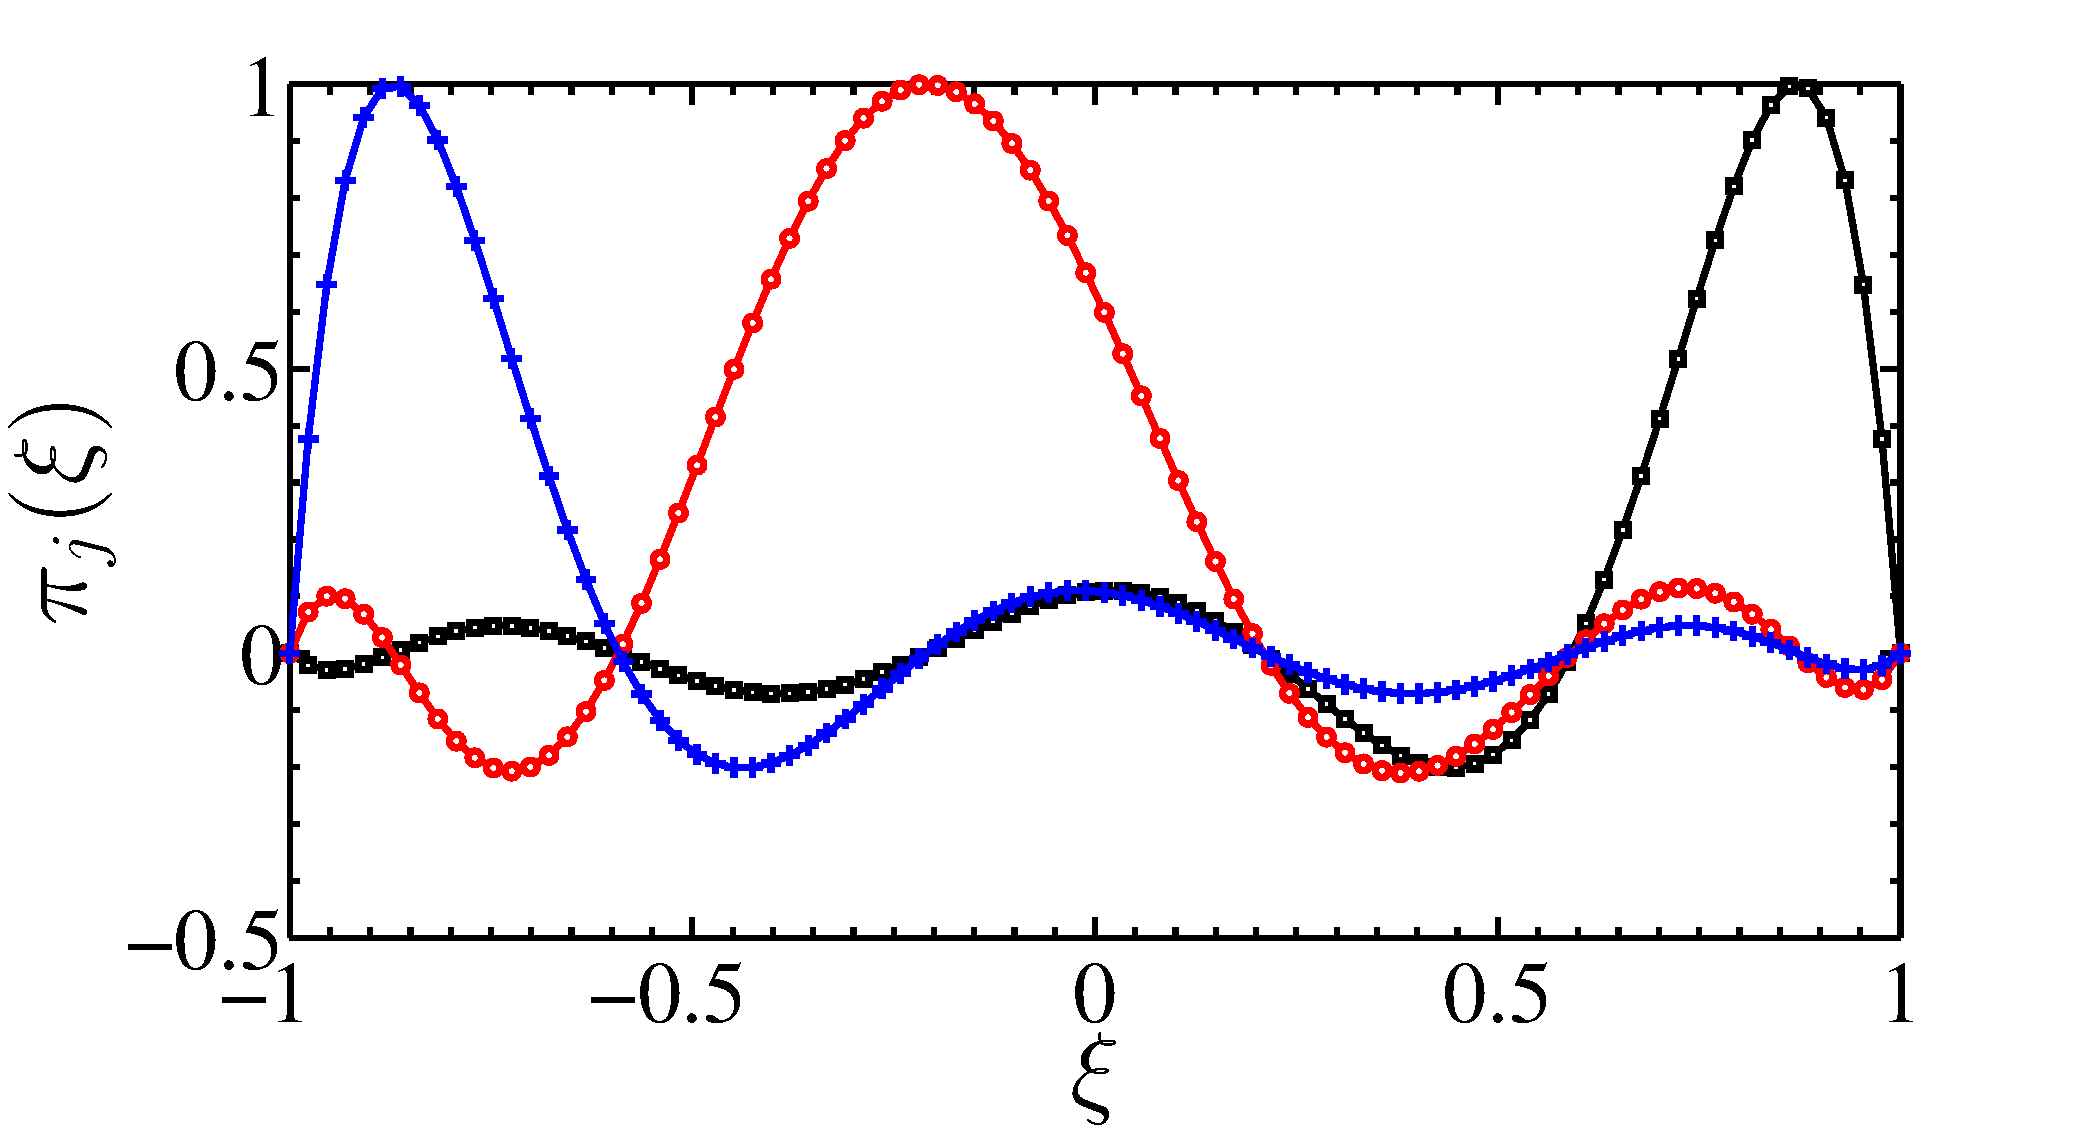
\includegraphics[width=\linewidth]{Figure/legpoly2.pdf}
                \caption{}
                \label{fig:poly1}
        \end{subfigure}
          \begin{subfigure}[b]{0.45\textwidth}
         \centering
                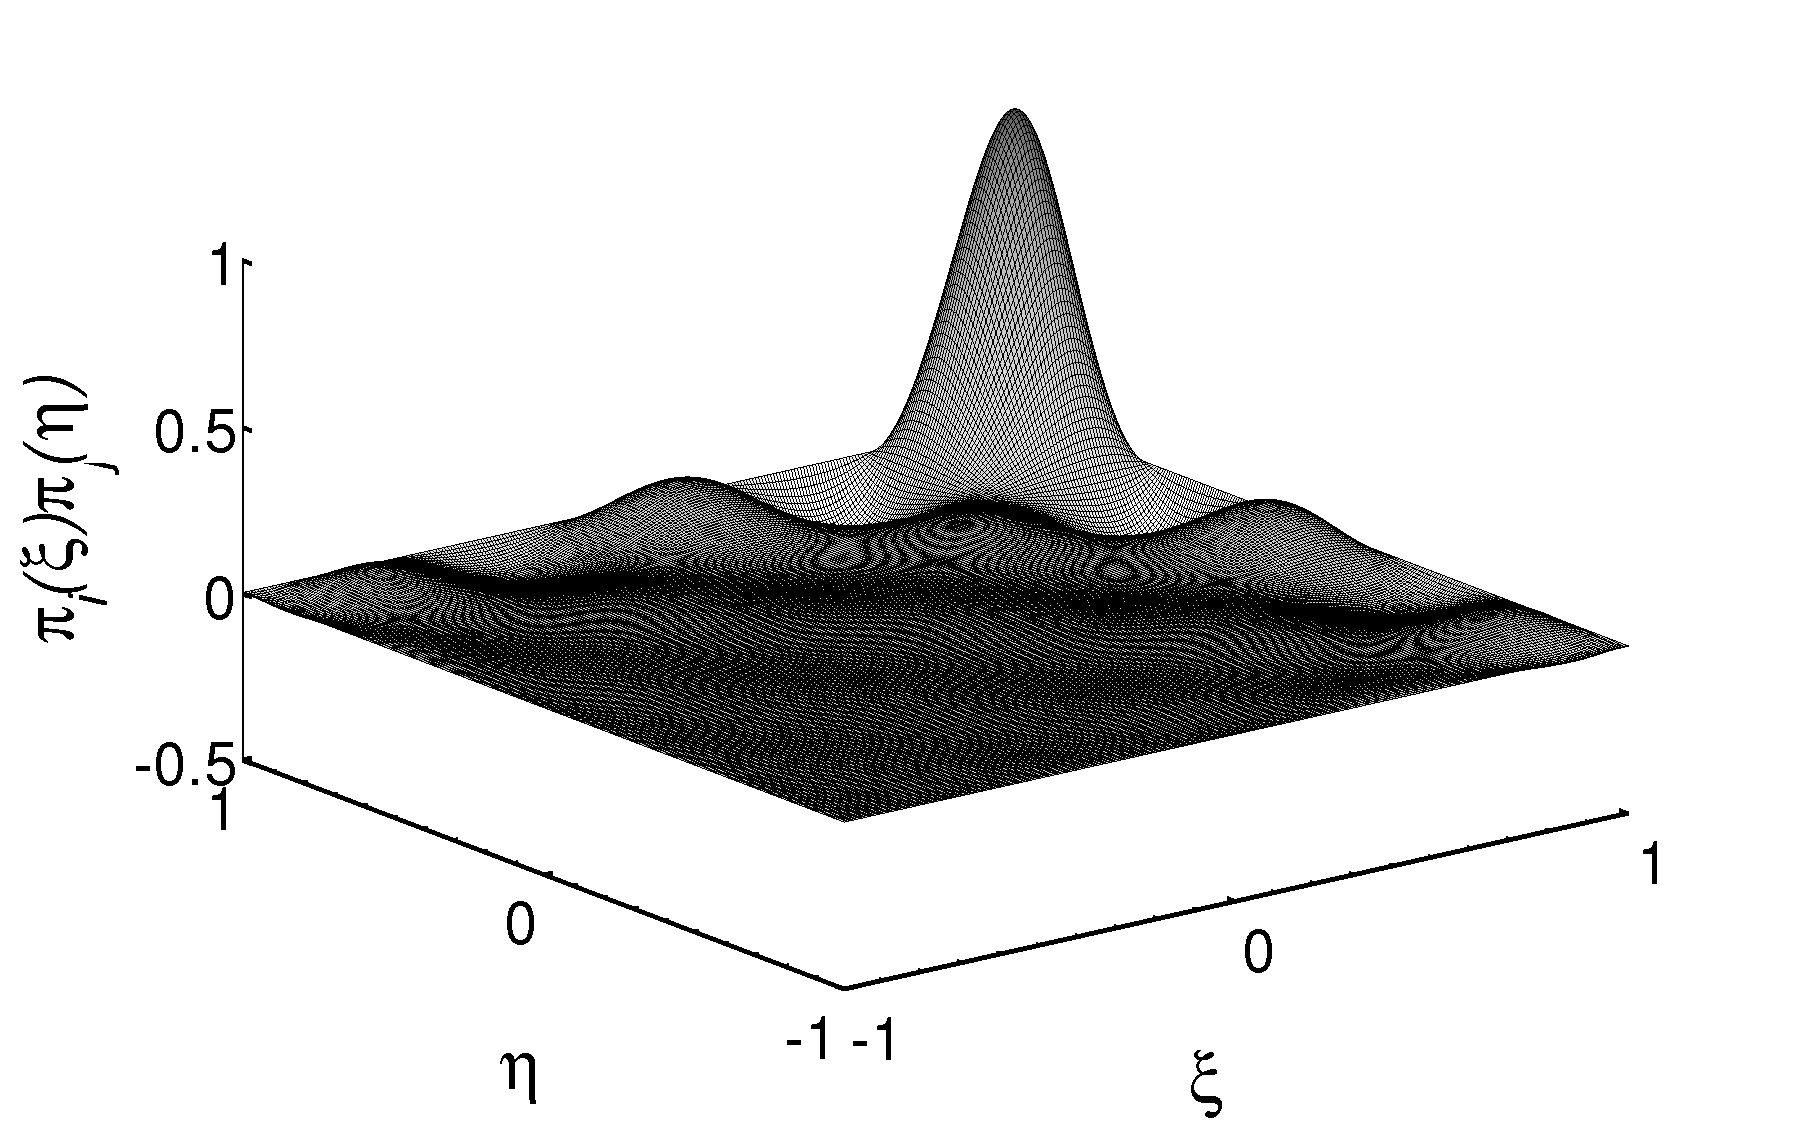
\includegraphics[width=\linewidth]{Figure/legpoly_2D1.pdf}
                 \caption{}
                 \label{fig:poly2}
         \end{subfigure}%
         \begin{subfigure}[b]{0.45\textwidth}
         \centering
                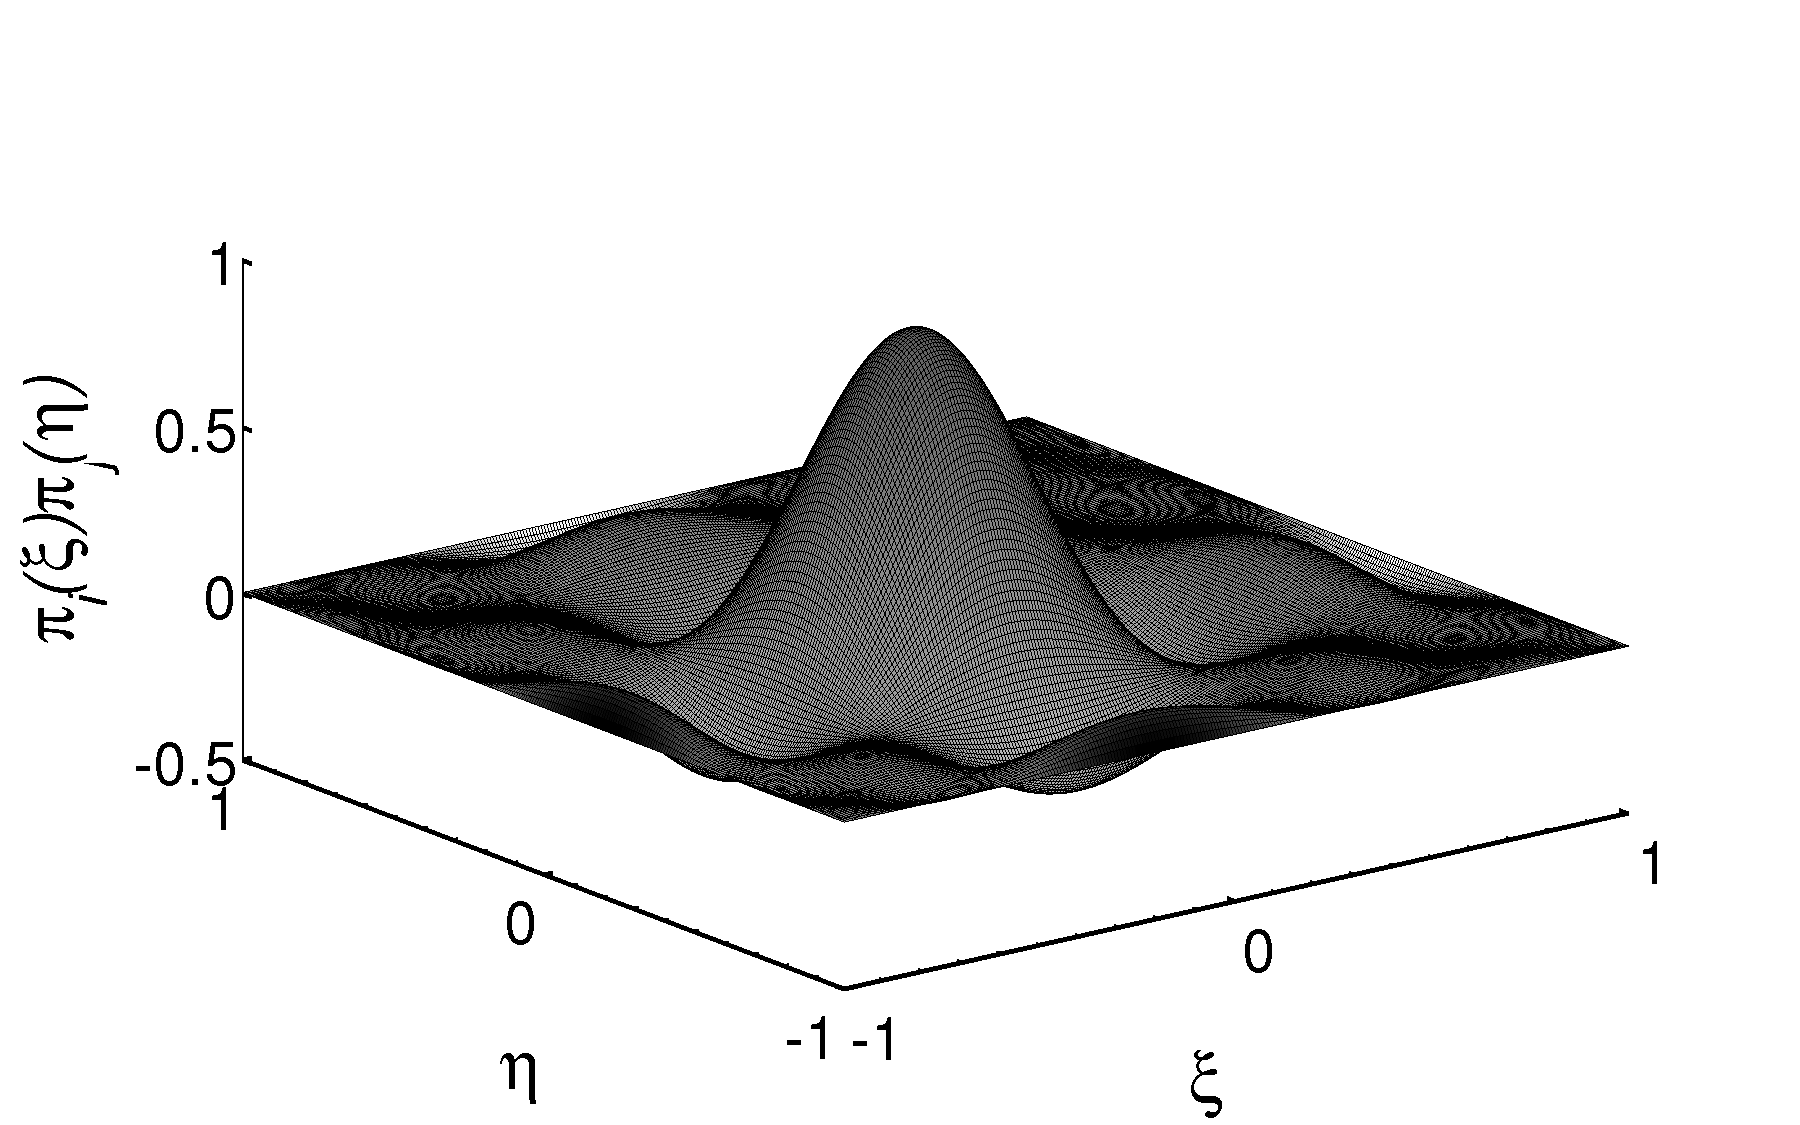
\includegraphics[width=\linewidth]{Figure/legpoly_2D2.pdf}
                 \caption{}
                 \label{fig:poly3}
         \end{subfigure}
        \caption{(a) Lagrange-Legendre polynomial interpolant ${\pi_j}_{j=0}^{N}$ with $N = 7\,(\mbox{polynomial degree})$ in current SEM formulation. Black-gray $--\ocircle$,   $\pi_0(\xi)$;  black $-\Box$,  $\pi_1(\xi)$;  black $--\Diamond$,  $\pi_2(\xi)$;  black $-.*$,  $\pi_3(\xi)$;  black-gray $--\davidsstar$  $\pi_5(\xi)$; gray-black $-$ \ding{72},  $\pi_6(\xi)$; black $+$, $\pi_7(\xi)$; $\pi_j(\xi_i) = \delta_{ij}$. (b)$\  \pi_{1,1}(\xi,\eta) \ \ $ (c) $\  \pi_{4,4}(\xi,\eta) \ $. Figures (b), (c) obtained as Kronecker products of $\pi_{i}(\xi)\otimes \pi_{j}(\eta)$ for 2D case.}\label{fig:figure_legpoly1}
\end{figure}

In spectral element methods~\cite{patera3},~\cite{deville},~\cite{fischer_jcp}, the decomposition of the computational domain consists of  subdividing $\bar{\Omega} = \Omega\cup \partial\, \Omega$ into $E$ non-overlapping adjacent rectilinear elements such that $\bar{\Omega} = \cup_{e=1}^{E}\Omega_{e}$. Each ${\Omega_{e}}$ is the image of a reference subdomain under a mapping\ ${\mathbf{x}}^{e}(\mathbf{r}) \in {\Omega_{e}} \rightarrow \mathbf{r}\in {\hat{\Omega}}$, with a well defined inverse  ${\mathbf{r}}^{e}(\mathbf{x}) \in \hat{{\Omega}} \rightarrow \mathbf{x}\in {\Omega_{e}}$, where the 3D reference subdomain is ${\hat{\Omega}} = [-1,1]^{3}$. Scalar functions within each local element ${{\Omega}_{e}}$ are represented as $N^{th}$ order tensor product polynomials on a reference subdomain ${\hat{\Omega}}$. With such decomposition, an elegant choice of the functional spaces of velocity and pressure fields as discussed before, commonly known as $\mathbb{P}_{N}-\mathbb{P}_{N-2}$ formulation are $X_N = X\cap \mathbb{P}_{N,E}^{3}$ and $Z_N = Z\cap \mathbb{P}_{N-2,E}$, where $\mathbb{P}_{N,E}$ can be given by
\begin{equation}
P_{N,E} = \left\{ \psi \ \Big|\ \psi \in L^2(\Omega); \:\:\psi|_{\Omega_e} \mbox{Lagrange-Legendre polynomial of degree} \leq N \right\}. \label{sob2}
\end{equation}
In 3D, velocity function in the spectral element method in the local element can be expressed as follows
\begin{equation}
u(r_1,r_2,r_3)|_{\hat{\Omega}} = \displaystyle\sum_{i=0}^{N_x}\sum_{j=0}^{N_y}\sum_{k=0}^{N_z}u_{ijk}^{e}\pi_{N_x,i}({r_1})\pi_{N_y,j}({r_2})\pi_{N_z,k}({r_3}),  \ \ \ {r_1},{r_2},{r_3}\in [-1,1]^3,
\end{equation}
where, $\pi_{N_x,i}(r_1),\hspace{0.5em} \pi_{N_y,j}(r_2), \hspace{0.5em}\pi_{N_z,k}(r_3)$ are the Lagrange polynomial based interpolant of degree $N_x$, $N_y$ and $N_z$ as in Equation(~\ref{legendre1}) satisfying the cardinality property $\pi_{N,i}(\xi_{j}) = \delta_{ij}$ where $\delta_{ij}$ is the Kronecker delta function.
 
Identically the pressure function in SEM in the local element, with $\pi^{p}_{N,j}({\zeta}) \in \mathbb{P}_{N-2}(\zeta)$ can be given as 
\begin{equation}
p(r_1,r_2,r_3)|_{\hat{\Omega}} = \displaystyle\sum_{i=1}^{N_x-1}\sum_{j=1}^{N_y-1}\sum_{k=1}^{N_z-1}p_{ijk}^{e}\pi^{p}_{N_x,i}({r_1})\pi^{p}_{N_y,j}({r_2})\pi^{p}_{N_z,k}({r_3}),  \ \ \ {r_1},{r_2},{r_3}\in [-1,1]^3
\end{equation}

It must be understood that due to an invertible mapping between $\Omega_{e}$ and $\hat{\Omega}$, there exists a one-to-one correspondence between the nodal values of $u(x,y,z)|_{\Omega_{e}}$, $p(x,y,z)|_{\Omega_{e}}$ and reference subdomain values $u(r_1,r_2,r_3)|_{\hat{\Omega}}$, $p(r_1,r_2,r_3)|_{\hat{\Omega}}$ and the coefficients $u_{ijk}^{e}$, $p_{ijk}^{e}$ are the local nodal values of $u|_{\Omega_{e}}$, $p|_{\Omega_{e}}$ respectively in this nodal-based formulation. The local to global mapping of data is carried out using a boolean connectivity matrix that preserves inter element continuity.

\subsection{Tensor products}
The differential operators in the current SEM formulation
%especially the poisson solvers in Nek5000
have been carried out using efficient implementation of tensor products~\cite{lynch},~\cite{orz}. The mapping of vector representation of the nodal coefficients $u_{ijk}^{e}$ is denoted by
\begin{equation}
\underline{u}^{e} = (u_{000}^e, u_{100}^e, \ldots , u_{ijk}^e, \ldots, u_{N_xN_yN_z}^e)^T=(u_1, u_2,\ldots, u_l, \ldots, u_{\mathcal{N}})^T 
\end{equation}
where $\mathcal{N} = (N_x+1)(N_y+1)(N_z+1)$ is the number of basis coefficients in a given element, and the mapping translates from three-index coefficient representation to a standard vector which is referred to as the natural or lexicographical ordering.

We denote $\hat{D}_x$ the matrix operator for the one dimensional derivative in $x$ direction; $\hat{D}_x$ is of size $(N_x+1)\times (N_x+1)$ obtained from the values of derivative of Lagrange-Legendre interpolating polynomial associated with $N_x + 1$ GLL points on the reference interval $[-1, 1]$ applied to each $N_x+1$-dimensional vector $(u_{0jk}^e,u_{1jk}^e, \ldots, u_{N_xjk}^e)^T$, $j = 0, \ldots, N_y$, $k = 0, \ldots, N_z$. We define analogously $\hat{D}_y$, $\hat{D}_z$ for one dimensional derivatives in $y,z$ direction.

Let us also define the Kronecker product of two matrices $A$ of size $k\times l$ and $B$ of size $m\times n$ as the matrix $C = A\otimes B$ of size $km\times ln$ given as 
\begin{equation}
c_{ij} = a_{pq}b_{rs},  \ \ \  0\le i\le km,  0\le j\le ln,
\end{equation}
where the index pairs $pq$ and $rs$ satisfy the relationships
\begin{equation}
i = r + (p-1)m ,      j = s + (q-1)n.
\end{equation}

 Based on the lexicographical ordering of $\underline{u}$, the block diagonal matrix format of the derivatives in $x,y,$ and $z$ direction as Kronecker or tensor product form can be given as $D_x = I_y\otimes I_z\otimes \hat{D}_x$, $D_y = I_x\otimes \hat{D}_y\otimes I_z$ and $D_z = \hat{D}_z\otimes I_x\otimes I_y$, where $I_x$ is the identity matrix of size $(N_x+1)\times (N_x+1)$ and so on. \\
\par
The block matrices formed by Kronecker products are advantageous since various important matrix operations required in SEM like matrix inversion, mapping transformation, eigenvalue calculations can be obtained by using these linear algebra operators on much smaller matrices than the global matrices~\cite{lynch},~\cite{deville}. Hence, tensor products are extremely computationally efficient in terms of parallel scalability when used in fast Poisson solvers, filtering and other linear operators in the current SEM methodology.\\

The time discretization of Navier-Stokes solver in the current spectral element code Nek5000~\cite{nek5000} involves $k^{th}$ order backward difference/extrapolation scheme (BDF/EXT) where $k = 2$ or $3$. The code is fully dealiased using $3/2$ rule~\cite{orz2,canuto}, the velocity  is solved using preconditioned conjugate gradient (CG) method and the pressure solver uses iterative generalized mean residual solver (GMRES) method in Krylov subspace.

\subsection{Large Eddy Simulation: Subgrid Scale modelling }
\label{LES}
The spatial-filtered Navier-Stokes equations for large eddy simulation can be written as
\begin{equation}
\frac{\partial \widetilde{u}_i}{\partial t} + \widetilde{u}_j\frac{\partial \widetilde{u}_i}{\partial x_j} = -\frac{1}{\rho}\frac{\partial \widetilde{p^{*}}}{\partial x_i} - \frac{\partial \tau^{\small SGS}_{ij}}{\partial x_j} + \widetilde{F_{i}}\delta_{1i} + \nu\frac{\partial^2\widetilde{u}_i}{\partial x_j \partial x_j} \label{leseq}
\end{equation}
where the ``tilde" represents the low-pass filtered variable and $\widetilde{u}_i$ is the instantaneous filtered velocity field in the $i^{th}$ direction. In this respect, we would like to point out that $x$ is the streamwise direction, $y$ is the spanwise direction and $z$ is the wall-normal direction of flow.\\
The modification to the original Navier-Stokes equations comes with an additional subgrid stress tensor which arises due to the non-commutativity of the convective term due to filtering, which is given by
\begin{equation}
\tau^{\tiny SGS}_{ij} = \widetilde{u}_i\widetilde{u}_j - \widetilde{{u}_i{u}_j}.
\end{equation}
The modified filtered pressure takes into account the trace of the subgrid stresses
\begin{equation}
\widetilde{p^{*}} = \widetilde{p} + \frac{1}{2}\widetilde{u}_{i}^2
\end{equation}
and $\widetilde{F_{i}}\delta_{1i}$ is the streamwise mean pressure gradient that drives the flow.
The assumption in this model is that the deviatoric part of the subgrid scale stress tensor can be modelled using standard Smagorinsky model (gradient diffusion/eddy viscosity hypothesis) in the filtered velocity field,
\begin{equation}
\tau^{SGS}_{ij} - \frac{1}{3}\tau^{SGS}_{kk}\delta_{ij} = 2(C_s\Delta)^2|\widetilde{S}|\widetilde{S}_{ij}, \label{sgs}
\end{equation}
where $\widetilde{S}_{ij} = \frac{1}{2}({\partial \widetilde{u}_i}/{\partial x_j}+ {\partial \widetilde{u}_j}/{\partial x_i})$ is the filtered strain rate and the magnitude of the strain tensor $|\widetilde{S}| = \sqrt{2\widetilde{S}_{ij}\widetilde{S}_{ij}}$. In classical Smagorinsky model~\cite{smagorinsky}, mixing length is assumed to be proportional to the grid filter width $\Delta$, and $C_s$ is the non dimensional Smagorinsky coefficient. The definition of grid filter width $\Delta = (\Delta_x\Delta_y\Delta_z)^{1/3}$ requires some caution for spectral element method. Karamanos et al.~\cite{karamanos} defined $\Delta_i = h_i/p$, with $i\in (x,y,z)$, where $h_i$ is the width of the element in the $i^{th}$ direction and $p$ is the order of the polynomial. The current SEM method uses a slightly different technique of calculating $\Delta = (\Delta x\Delta y\Delta z)^{1/3}$, where $\Delta x, \Delta y, \Delta z$ are calculated as central difference between GLL nodes at the interior and one sided difference at the boundaries followed by an average across the inter element boundaries. Lily (1967)~\cite{lily0} predicted Smagorinsky coefficient $C_s \sim 0.16$ for isotropic turbulence from the equilibrium of subgrid dissipation and viscous dissipation. However, wall-bounded or mean sheared flows, have shown a sensitive dependance of $C_s$ on the magnitude of shear, and a $C_s \sim 0.16$  was overly dissipative in the near wall region, damping large-scale fluctuations and restricting the near wall coherent eddies to develop that aid in turbulent transport~\cite{hor,bers}. Consequently, such high values of Smagorinsky coefficient predicted unrealistic slopes of the mean velocity profile (mean shear), which is commonly known as the ``log-layer mismatch" (deviation of the mean velocity profile from the logarihtmic trends)~\cite{andren,meyers2}. In Channel flow simulations various $C_s$ has been reported in the literature, e.g. $C_s \approx 0.1$~\cite{deardoff}, $C_s \approx 0.09$~\cite{bardina2}, while~\cite{moin1} reported $C_s \approx 0.065$ for acceptable results. However, simple reduction of $C_s$ is not good enough, since near wall physics also requires that the mixing lengths and hence $C_s$ are damped near the wall such that it can capture the dynamics of near wall eddies.\\
For high Reynolds number turbulent ABL flow, we use algebraic wall damping by Mason and Thompson (1992)~\cite{mason}.
\begin{equation}
\frac{1}{(C_s\Delta)^{n}} = \frac{1}{(C_s\Delta)^{n}} + \frac{1}{\kappa(z + z_0)^{n}} \label{mas}
\end{equation} 
Equation(~\ref{mas}) essentially uses an ad-hoc blending function with parameters $C_0, n$, such that at outer layer, it has conventional Smagorinsky based mixing length scales for SGS stress, while it retrieves scales corresponding to the log-law $\sim \kappa z$ as it approaches near-wall~\cite{mason0,mason} ($\kappa \approx 0.41$ is the Von-Karman constant and will also be used in the subsequent sections). This algebraic damping function can be viewed analogous to the Van-Driest damping function~\cite{van-Driest,bers} for smooth wall-resolved LES. Various values of parameter $C_0, n$ has been reported in the literature, e.g. Port$\acute{e}$-Agel uses $C_s = 0.1-0.17$, $n = 1,2$ respetively, while Calaf and Meyers~\cite{calaf} published $C_s = 0.13$ and $n = 3$ for their simulations. However, using these values without tuning is problematic in spectral element methods, since these values are mostly used in conjuntion with 2nd order central difference~\cite{porte1fun,porte1a}, or 4th order conservative finite difference~\cite{meyers2} in the wall normal direction, which are extremely dissipative and dispersive as compared to the exponentially accurate SEM. Using these values directly, in SEM would result in vigorous wall normal spatial oscillation in the near-wall region for the resolved kinematic shear stress. Considering this , we always use $C_s \sim 0.15-0.17$, with $n = 2, 3$ in our current spectral element simulations without invoking too much numerical error into the system. It is also important to note that the Smagorinsky coefficient with algebraic wall damping can also be written as
\begin{equation}
C_s = (C_0^{-n} + \{\kappa(\frac{z}{\Delta} + \frac{z_0}{\Delta})\}^{-n})^{1/n}
\end{equation}
\begin{figure}
       \centering
          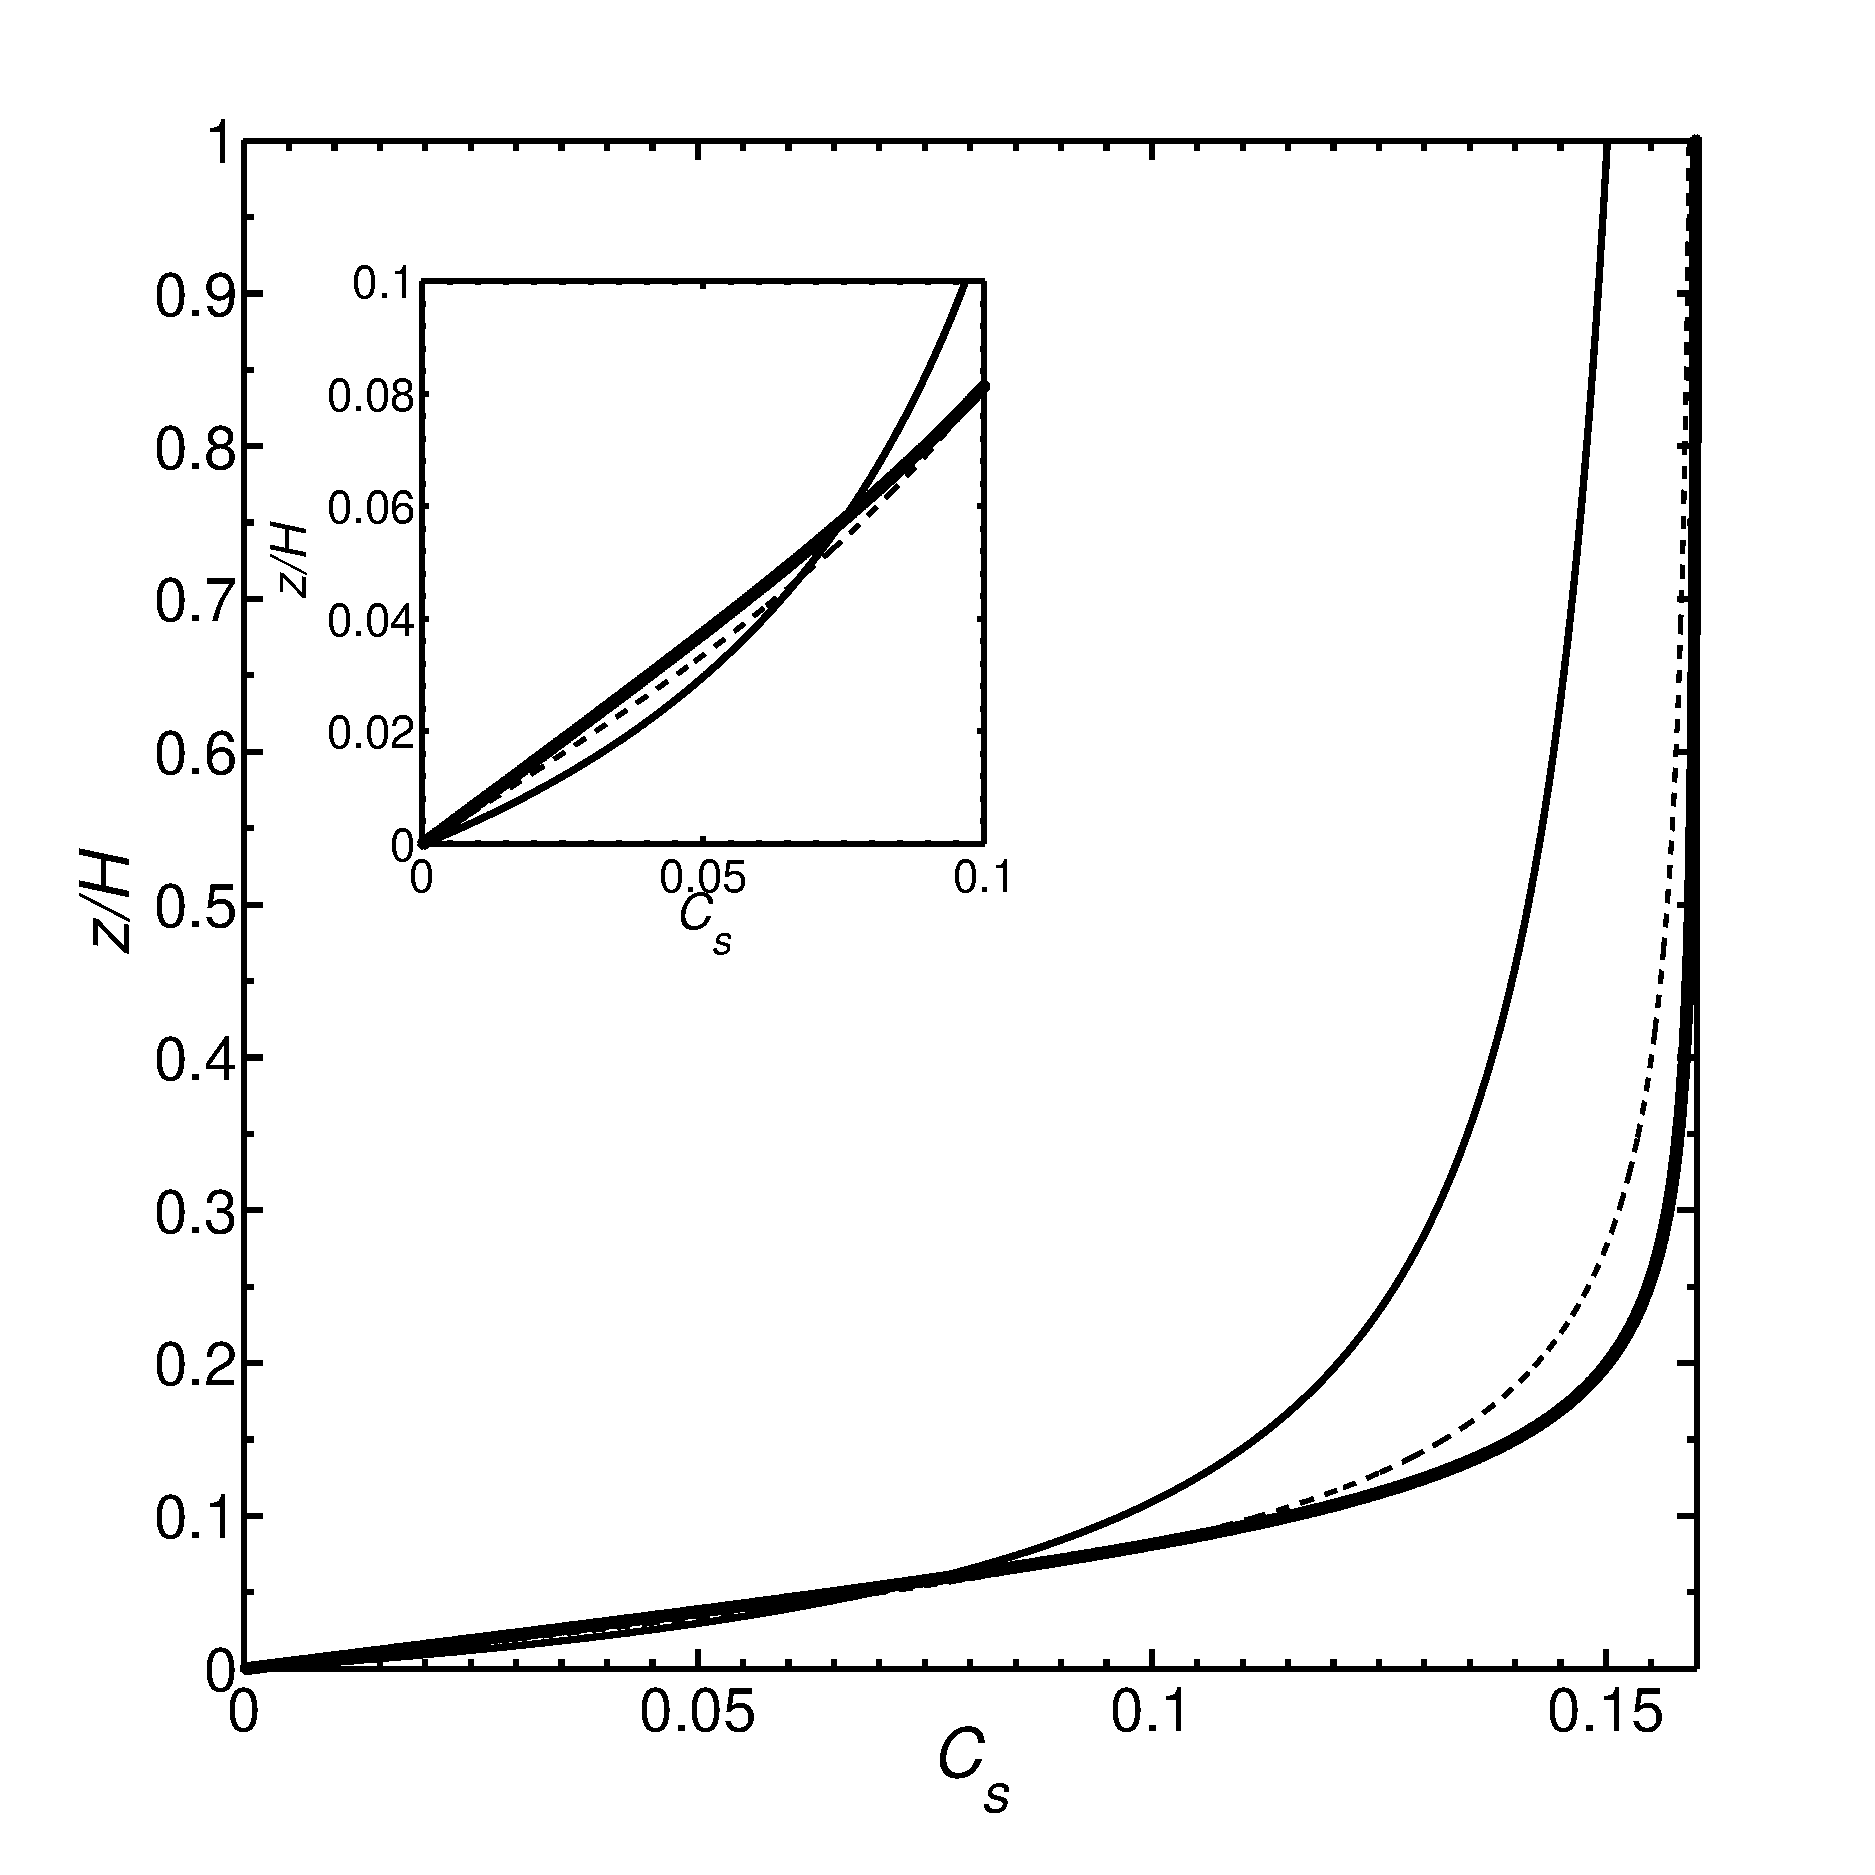
\includegraphics[width= 65.5mm]{Figure/Smag.pdf}
       \caption{Smagorinsky coefficient $C_s$ vs $z/H$. $-$ black, $n = 1$; $--$ black, $n = 2$; $\star$ black, $n = 3$. $C_0 = 0.16$, fixed. $\kappa = 0.41$, Von Karman constant. $z_0 = 0.0002$. Inset: variation of $C_s$, zoomed-in. }
\label{fig:figure_smag}
\end{figure}

The formulation clearly reveals that  $C_s \sim f(z/\Delta)$ which manifest the effect of static/ad-hoc scale dependence of the Smagorinsky coefficient at fixed height above the ground~\cite{porte1fun,bou1}. The effect of rough-wall $z_0$ can be explicitly seen in Equation(~\ref{mas}). Figure~\ref{fig:figure_smag} shows the variation of Smagorinsky coefficient $C_s$ as a function of $z/H$, where $H$ is the boundary layer thickness. It is interesting to note, that with this SGS model, SGS dissipation can be observed even at the approximate boundary with a mixing length $\sim \kappa z_0$. It is also observed from Figure~\ref{fig:figure_smag}, that increasing $n$ tends to sharpen the blending function in algebraic damping near wall. This is essential, since, with higher value of $n$, the Smagorinsky models, better represent the log law region (mixing length $\sim \kappa z$) and reaches the classical Smagorinsky coefficient at a shorter wall-normal height. Figure~\ref{fig:figure_smag} also justifies the use of higher value of $C_s$ ($C_s|_{n=1} > C_s|_{n=2}$), when using low value of $n$ to keep the dissipation length scales approximately of the same magnitudes (same $C_s$) in the log-law and outer layer.


\subsection{Near Wall model: approximate boundary conditions}\label{nwm}
 The mean streamwise velocity profile of ABL  in the surface layer (roughly $10 \sim 20\%$ of boundary layer)~\cite{basin,porte1fun,meyers} can be given as
\begin{equation}
\bar{U}(z) = \frac{u_{\tau}}{\kappa}\ln \frac{z}{z_0} + \frac{u_{\tau}}{\kappa}\psi_m(\frac{z}{L_M}),\ \ \  z \gg z_0  \label{logvel}
\end{equation}
where, $u_\tau$ is the friction velocity scale, $z_0$ is the aerodynamic roughness length and $\kappa = 0.4$ is the Von Karman constant, $\psi_m$ is a non dimensional momentum stability function and $L_M$ is stability length scale by Monin and Obukhov.~\cite{obu,basin}. Since we propose to simulate high Reynolds number neutral ABL flows, $L_M\rightarrow \infty$ and hence the mean velocity profile is essentially logarithmic in nature in the surface layer~\cite{obu,porte1fun,meyers2} with $\psi_m \rightarrow 0$.\\
 We choose neutral ABL for our simulation model, because it is simplest in terms of computation compared to stratified or convective ABL models where $L_M$ is non-zero, and its parametrization may be complicated ~\cite{moeng1,basin}. For the current neutral ABL simulation, the length scale of the computational domain is small enough and hence the Coriolis force has been neglected for the present purpose. Moreover, since we perform neutral stability calculations, additional terms to account for buoyancy or stratification effects have been ignored as well. Neutral ABL flows can serve as a best approximation for the boundary layer when the sky is overcast with clouds for significantly long period of time. \\
\par
At extremely high Reynolds number, $Re \sim 10^8- 10^{14}$, the growth of boundary layer ($d\delta_{bl}/dx \sim O(Re^{-p})\approx 0,\ \ p \geqslant 1$) becomes infinitesimally small. Consequently we incorporate periodic boundary conditions in the streamwise direction enforcing homogeneity in the system. Periodic boundary conditions are also invoked in the spanwise direction since it is consistent with the physics of the flow. Boundary conditions in the top is stress free lid $d\widetilde{u}_{i}/dz = 0, i = 1,2\ \ \mbox{and} \ \ \widetilde{u}_{i} = 0, i = 3$ to emulate flat plate boundary layer analogy.\\
We now discuss in details the approximate boundary conditions at the bottom ``wall". For that we look back into Equation($~\ref{weak1}$) and concentrate on the weak-formulation of the viscous diffusion term derived from the integration by parts of the Laplacian, $\nu\int_{\Omega}\nabla \mathbf{u}.\nabla \mathbf{v}d^{3}\mathbf{x}$ with $v$ being the test function. A straightforward simplification reveals, that the term can be further broken down to  $\nu\int_{\Omega}\nabla^{s} \mathbf{u}.\nabla^{s} \mathbf{v}d^{3}\mathbf{x}$. The expression essentially projects the viscous flux into the test space in weak formulation, where $2\nabla^{s}() = \nabla() + \nabla()^{T}$ is the symmetric gradient operator. The full integration would involve data from surface of the domain $\partial \Omega$ and $\nu\nabla^{s} \mathbf{u}|_{\partial \Omega}$ can be easily closed using a closure model for the momentum flux. From now onwards, we refer to the momentum flux (shear stress) with the notation $\tau_{,s}$ for brevity. The shear stress boundary conditions for near-wall modelling are calculated from the ``in-phase" filtered resolved velocity fields half a grid node away from the ``wall" satisfying log-law (also from Monin-Obukov similarity theory)~\cite{obu}.
\begin{equation}
\tau_{i,zs} = -\kappa^{2}\frac{\widehat{\widetilde{u}}_{i,\frac{\Delta z}{2}}(x,y,t)\widehat{\widetilde{u}}_{r,\frac{\Delta z}{2}}(x,y,t)}{\log (\frac{z}{z_0})|_{\frac{\Delta z}{2}}^{2}} \ \ \ \  \forall i = x,y \label{stress}
\end{equation}
The subscript ``s" represents shear stress at the wall surface and the ``tilde" in Equation(~\ref{stress}) represents implicit grid filtering in LES, while in SEM, the explicit filtering represented by the ``hat" is carried out in modal space by attenuating $n$ (usually 2--4) highest Legendre polynomial modes.The explicit filtering is done in an effort to minimize the log-layer mismatch
(overshoot of slope of logarithmic mean velocity profile observed in high $Re$ flows)~\cite{bou1,meyers2}. Similar trends of incorrect slopes in logarithmic profiles has been observed by Piomelli and Ballaras~\cite{pio2} at lower Reynolds number ($Re\sim 10^6$) than current computation using LES and DES (detached-eddy simulation, wall-layer RANS) which has been attributed to the artificial eddies being generated in the wall-outer layer~\cite{bag2}. This is intriguing to note, since wall-layer model also essentially considers the near wall region in the Reynolds average sense~\cite{pio2,jimtech,lars}.
\begin{equation}
\widehat{\widetilde{u}}_{r,\frac{\Delta z}{2}} = \sum_{i}\sqrt{\widehat{\widetilde{u}}_{i,\frac{\Delta z}{2}}^{2}} \ \ \ \ \ \ \ \forall i = x,y
\end{equation}
For collocated spectral element methods $\widehat{\widetilde{u}}_{i,r,\frac{\Delta z}{2}}$ are calculated as an interpolation at half wall node $\Delta z/2$ between $\widehat{\widetilde{u}}_{i,r}(x,y,0,t)$ and $\widehat{\widetilde{u}}_{i,r}(x,y,z=\Delta z,t)$. Various types of interpolation has been incorporated in the present calculations involving simple mid-point ($1^{st}$ order), logarithmic (to mimic logarithmic velocity profile at wall) and exponentially accurate spectral interpolation technique, the detail comparisons of which have been discussed in Section~\ref{results}. Earlier cited literature on near wall modelling~\cite{deardoff,schumann,grot,moeng1,pio_wall,bal2,porte1fun,meyers2} have generally used staggered finite-difference schemes ($2^{nd}$ to $4^{th }$ order) when using stress boundary conditions for rough wall models with $\Delta z/2$ being a physical grid distance away from the wall (since the pressure and velocity grids are different). The present paper incorporates a relatively new robust model for rough wall using spectral element methods~\cite{tan}, and consequently certain modifications in the conventional rough-wall models of the cited-researchers have been introduced in Equation(~\ref{stress}). It is quite fascinating to note the striking  similarity in implementation between the flux conservative finite volume/ finite difference methods, and the weak formulation of collocated SEM, where the wall model essentially is a flux-closure scheme.
The aerodynamic roughness length $z_0$ in Equation(~\ref{stress}) is a monotonic measure of physical surface roughness $h$ and their empirical relations are discussed in literature~\cite{bhag,taft,cast}. The friction velocity scale is given by $u_{\tau} = \sqrt{{\tau_{w}}/{\rho}}$, where $\tau_{w}$ is the wall shear stress, $\widetilde{F_{i}}\delta_{1i}$ (Equation(~\ref{leseq})) is the streamwise pressure gradient that drives the ABL flow, $H$ is the depth of the boundary layer and $\rho$ is the fluid density, which can be further simplified as follows

\begin{equation}
\tau_{w} = \sqrt{\tau_{x,zs}^{2} + \tau_{y,zs}^2} = \bigg(\frac{\kappa}{\log (\frac{\Delta z}{2z_0})}\bigg)^{2}\widehat{\widetilde{u}}_{r,\frac{\Delta z}{2}}^{2} = \widetilde{F}_{1}H \label{stress2}
\end{equation}

The parametrization of wall shear stress in Equation(~\ref{stress},~\ref{stress2}) reveals that the shear stress can be modelled for simpler geometries using ``law of the wall" since the filtered velocity information can be taken from the core logarithmic region. The near wall model in the current paper, neglects the effects of pressure gradients, unsteadiness and streamline curvature, which are observed in instantaneous LES flow fields. Moreover, logarithmic trend of velocity profile is only justified with its mean, and it is quite inappropriate to apply the same for instantaneous variables. Consequently, an explicit filtering in addition to LES implicit grid filtering has been employed to partially circumvent the situation~\cite{bou1,meyers2}.\\
 The computational domain for ABL simulation has been chosen to be $L_x = 4\pi\delta$, $L_y = 2\pi\delta$ and $L_z = 2\delta$, and $2\delta$ is the boundary layer thickness. The choice of the streamwise domain is crucial since it should be large enough such that the auto-correlation length scale decays significantly to make the periodic boundary conditions consistent~\cite{kimmoinmoser,pope}. Previous literature in Channel-flow and ABL flow simulations have reported stream-wise spanwise geometry in terms of multiples of boundary layer thickness respectively as $2\pi, \ \pi$ ~\cite{kimmoinmoser,porte1a}, $2\pi, \ 2\pi/3$~\cite{porte2a} and $2\pi, \pi$~\cite{meyers2}. We have considered the smallest domain possible to optimise the computational expense. The aerodynamic roughness has been taken to be $z_0 = 10^{-4}H$, similar to the past literature~\cite{porte2a,meyers2}. The domain has been uniformly discretized using $X Y Z$ elements ($1^{st}$ wall grid-mode lies on the log-layer) and the order of the polynomial chosen for the present purpose is $N = 7$, which is optimum~\cite{nek5000} since with low values of $N\sim 4-6$, the effects of dissipation and dispersion errors starts creeping in, and using higher-order polynomials $N\sim 10-12$ increases the computational cost significantly without improving on the accuracy of LES results.  \\
\subsubsection{Element level filtering in SEM}\label{element_level}
\vspace{3 mm}
:\hspace{5mm} For the explicit filtering approach in near-wall modelling we use the modal approach of Boyd~\cite{boyd3}, see also~\cite{black}, \cite{bouf}. With the modal filtering technique, decomposition of the variable $u$ into the modal basis is sought,
\begin{equation}
u(\xi_i) = \sum_{k=0}^N{\hat{u}_k\phi_k(\xi_i)},\label{eq:modal}
\end{equation}
where $\xi_i, i = 0, \cdots, N$ represent the GLL clustering of the nodes, and the modal basis $\{\phi\}$,
\begin{equation}
\phi_0 = L_0(\xi),\ \ \phi_1 = L_1(\xi) \ \ \ \mbox{and}\ \ \ \ \phi_k = L_k(\xi) - L_{k-2}(\xi), \ \ \ 2\le k\le N  
\end{equation}
forms the hierarchical set of functions constructed from the Legendre polynomials $L_k(\xi)$. Although the Legendre polynomials are normalized, satisfying $L_k(\pm 1) = (-1)^k$, the bubble functions $\phi_k$, on the other hand, are designed to preserve homogeneous Dirichlet boundary conditions, since $\phi_k(\pm 1) = 0$ for $k\geq2$. The inhomogeneous Dirichlet boundary conditions are satisfied by the low order polynomials $\phi_0, \phi_1$. The mapping between the nodal Lagrangian basis and the modal representation defined by Eq.~(\ref{eq:modal}) can be cast into the matrix form\begin{equation}
\mathbf{u} = \Phi \mathbf{\hat{u}}.
\end{equation}
%The filtered function $\tilde{u}(\xi) = \sum_{k = 0}^{N}\sigma(k;N)\hat{u}_k\phi_k(\xi)$, with $\sigma$ being the filtered coefficient, in matrix-vector format are elegantly presented below as \\

\begin{figure}
\centering
        \begin{subfigure}[b]{0.32\textwidth}
                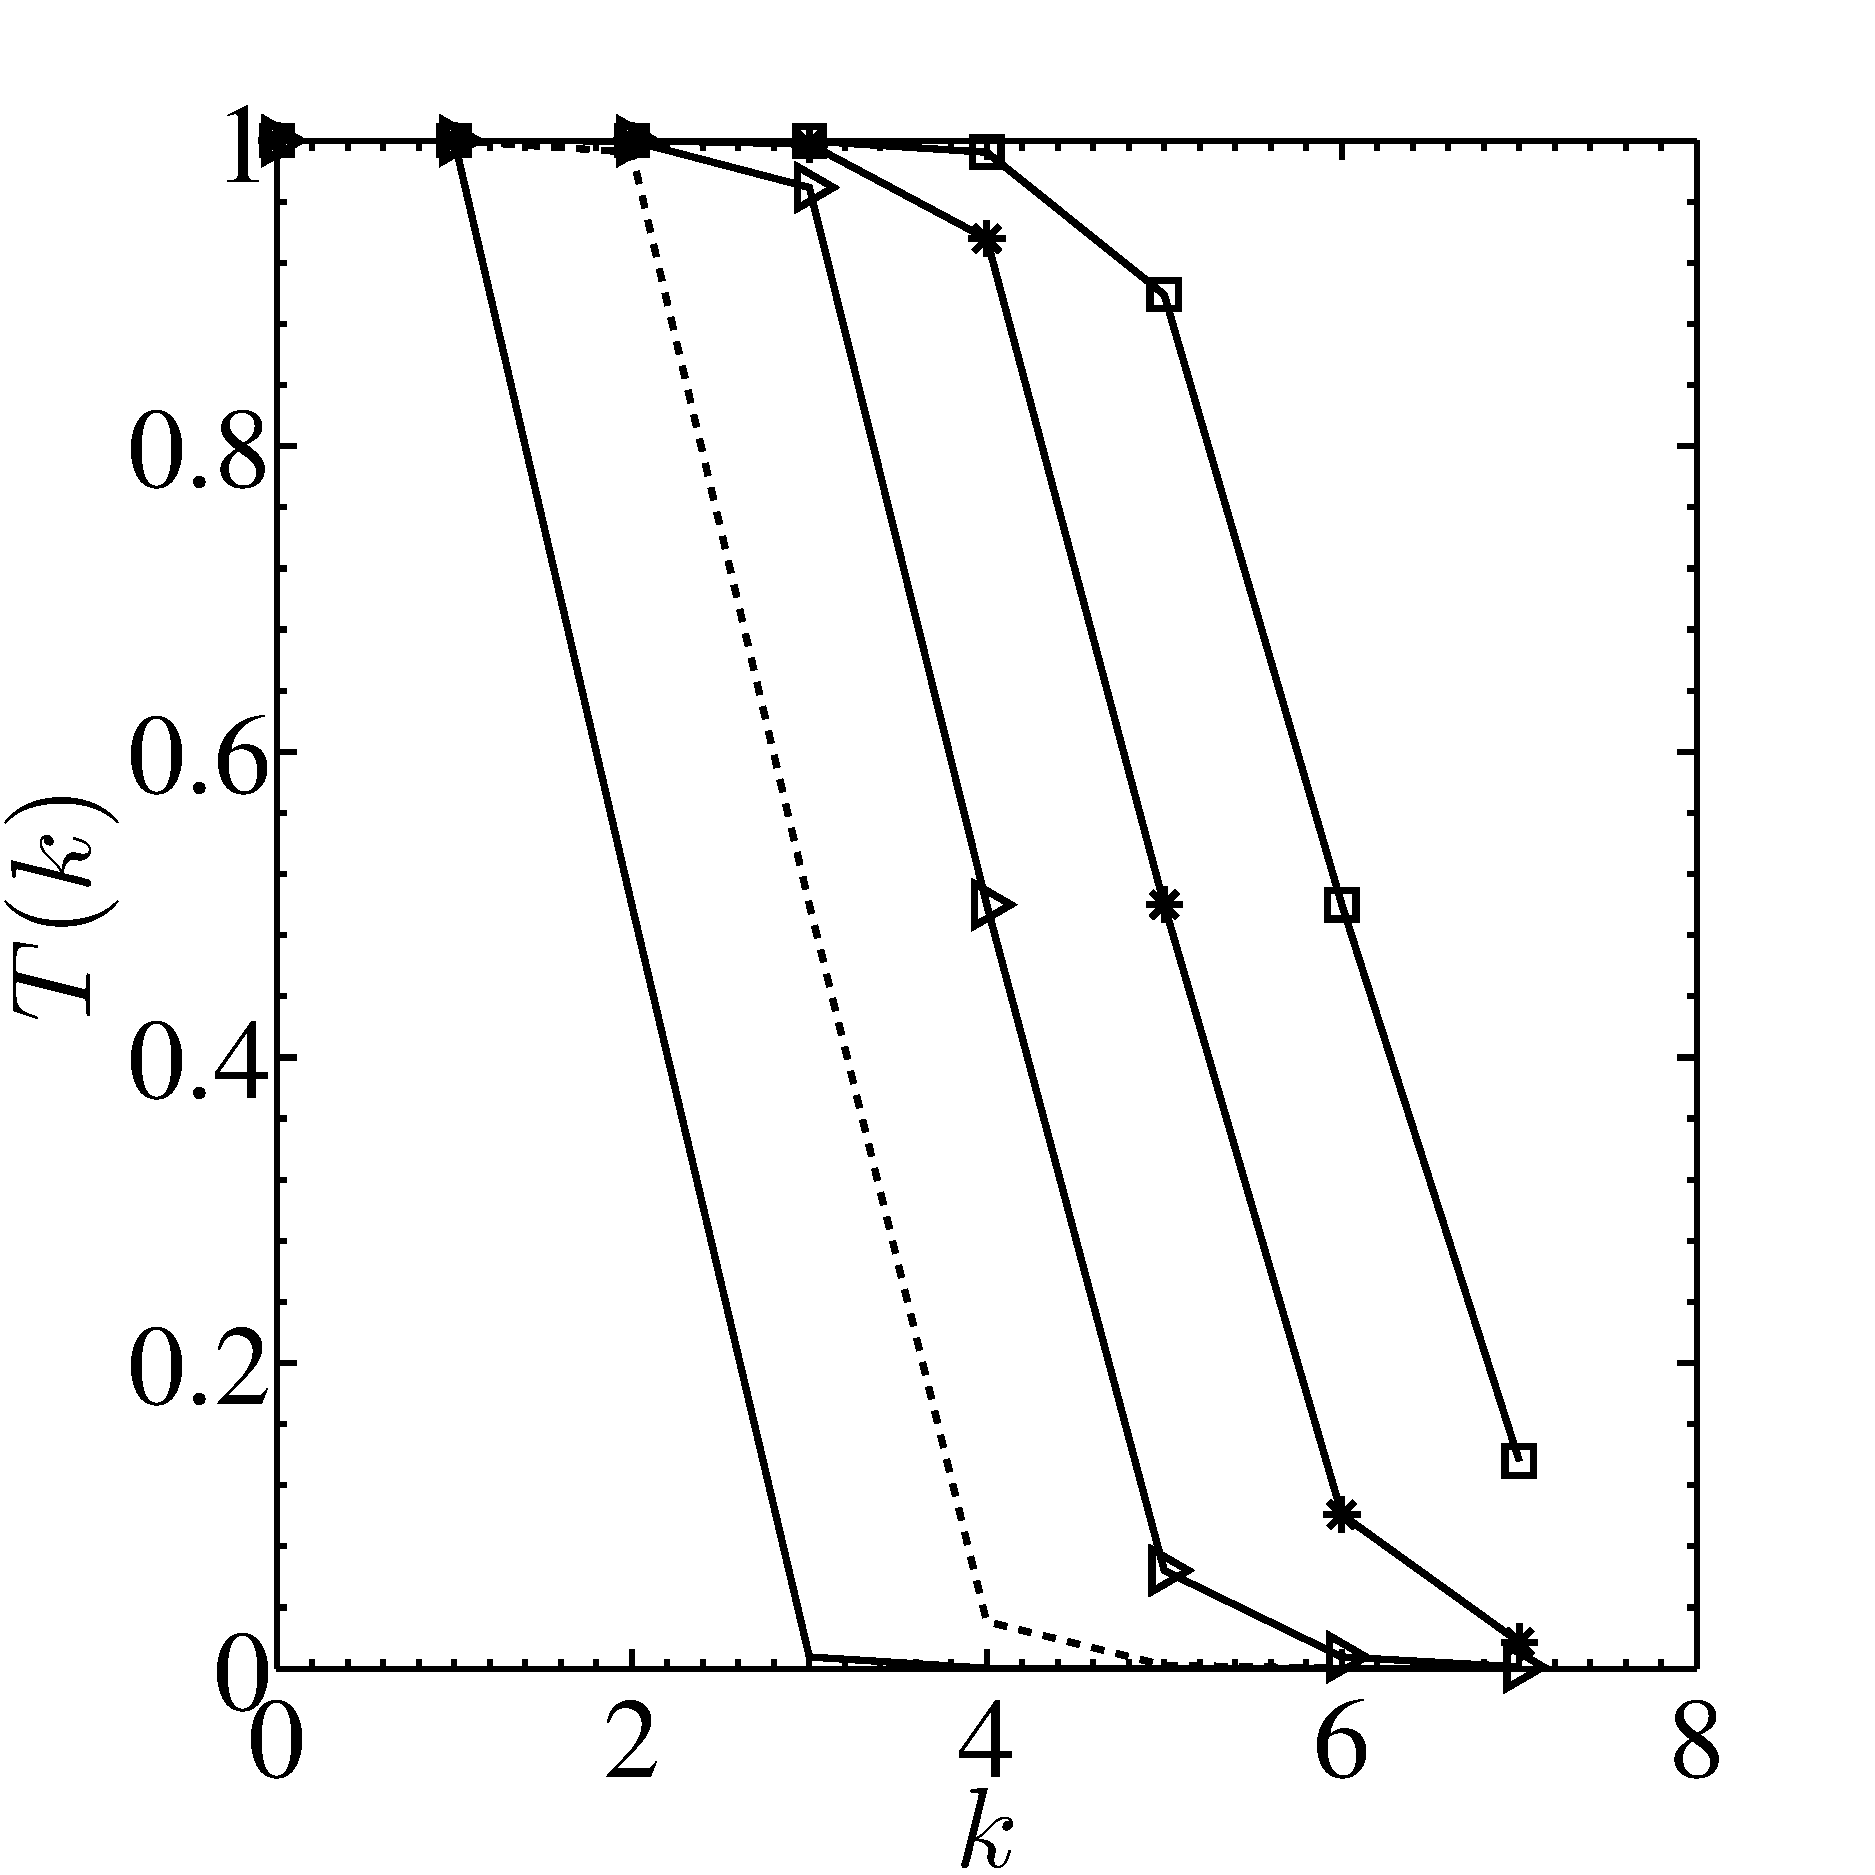
\includegraphics[width=\linewidth]{Figure/filter1.pdf}
                \caption{}
                \label{fig:filt1}
        \end{subfigure}%
          \begin{subfigure}[b]{0.32\textwidth}
         \centering
                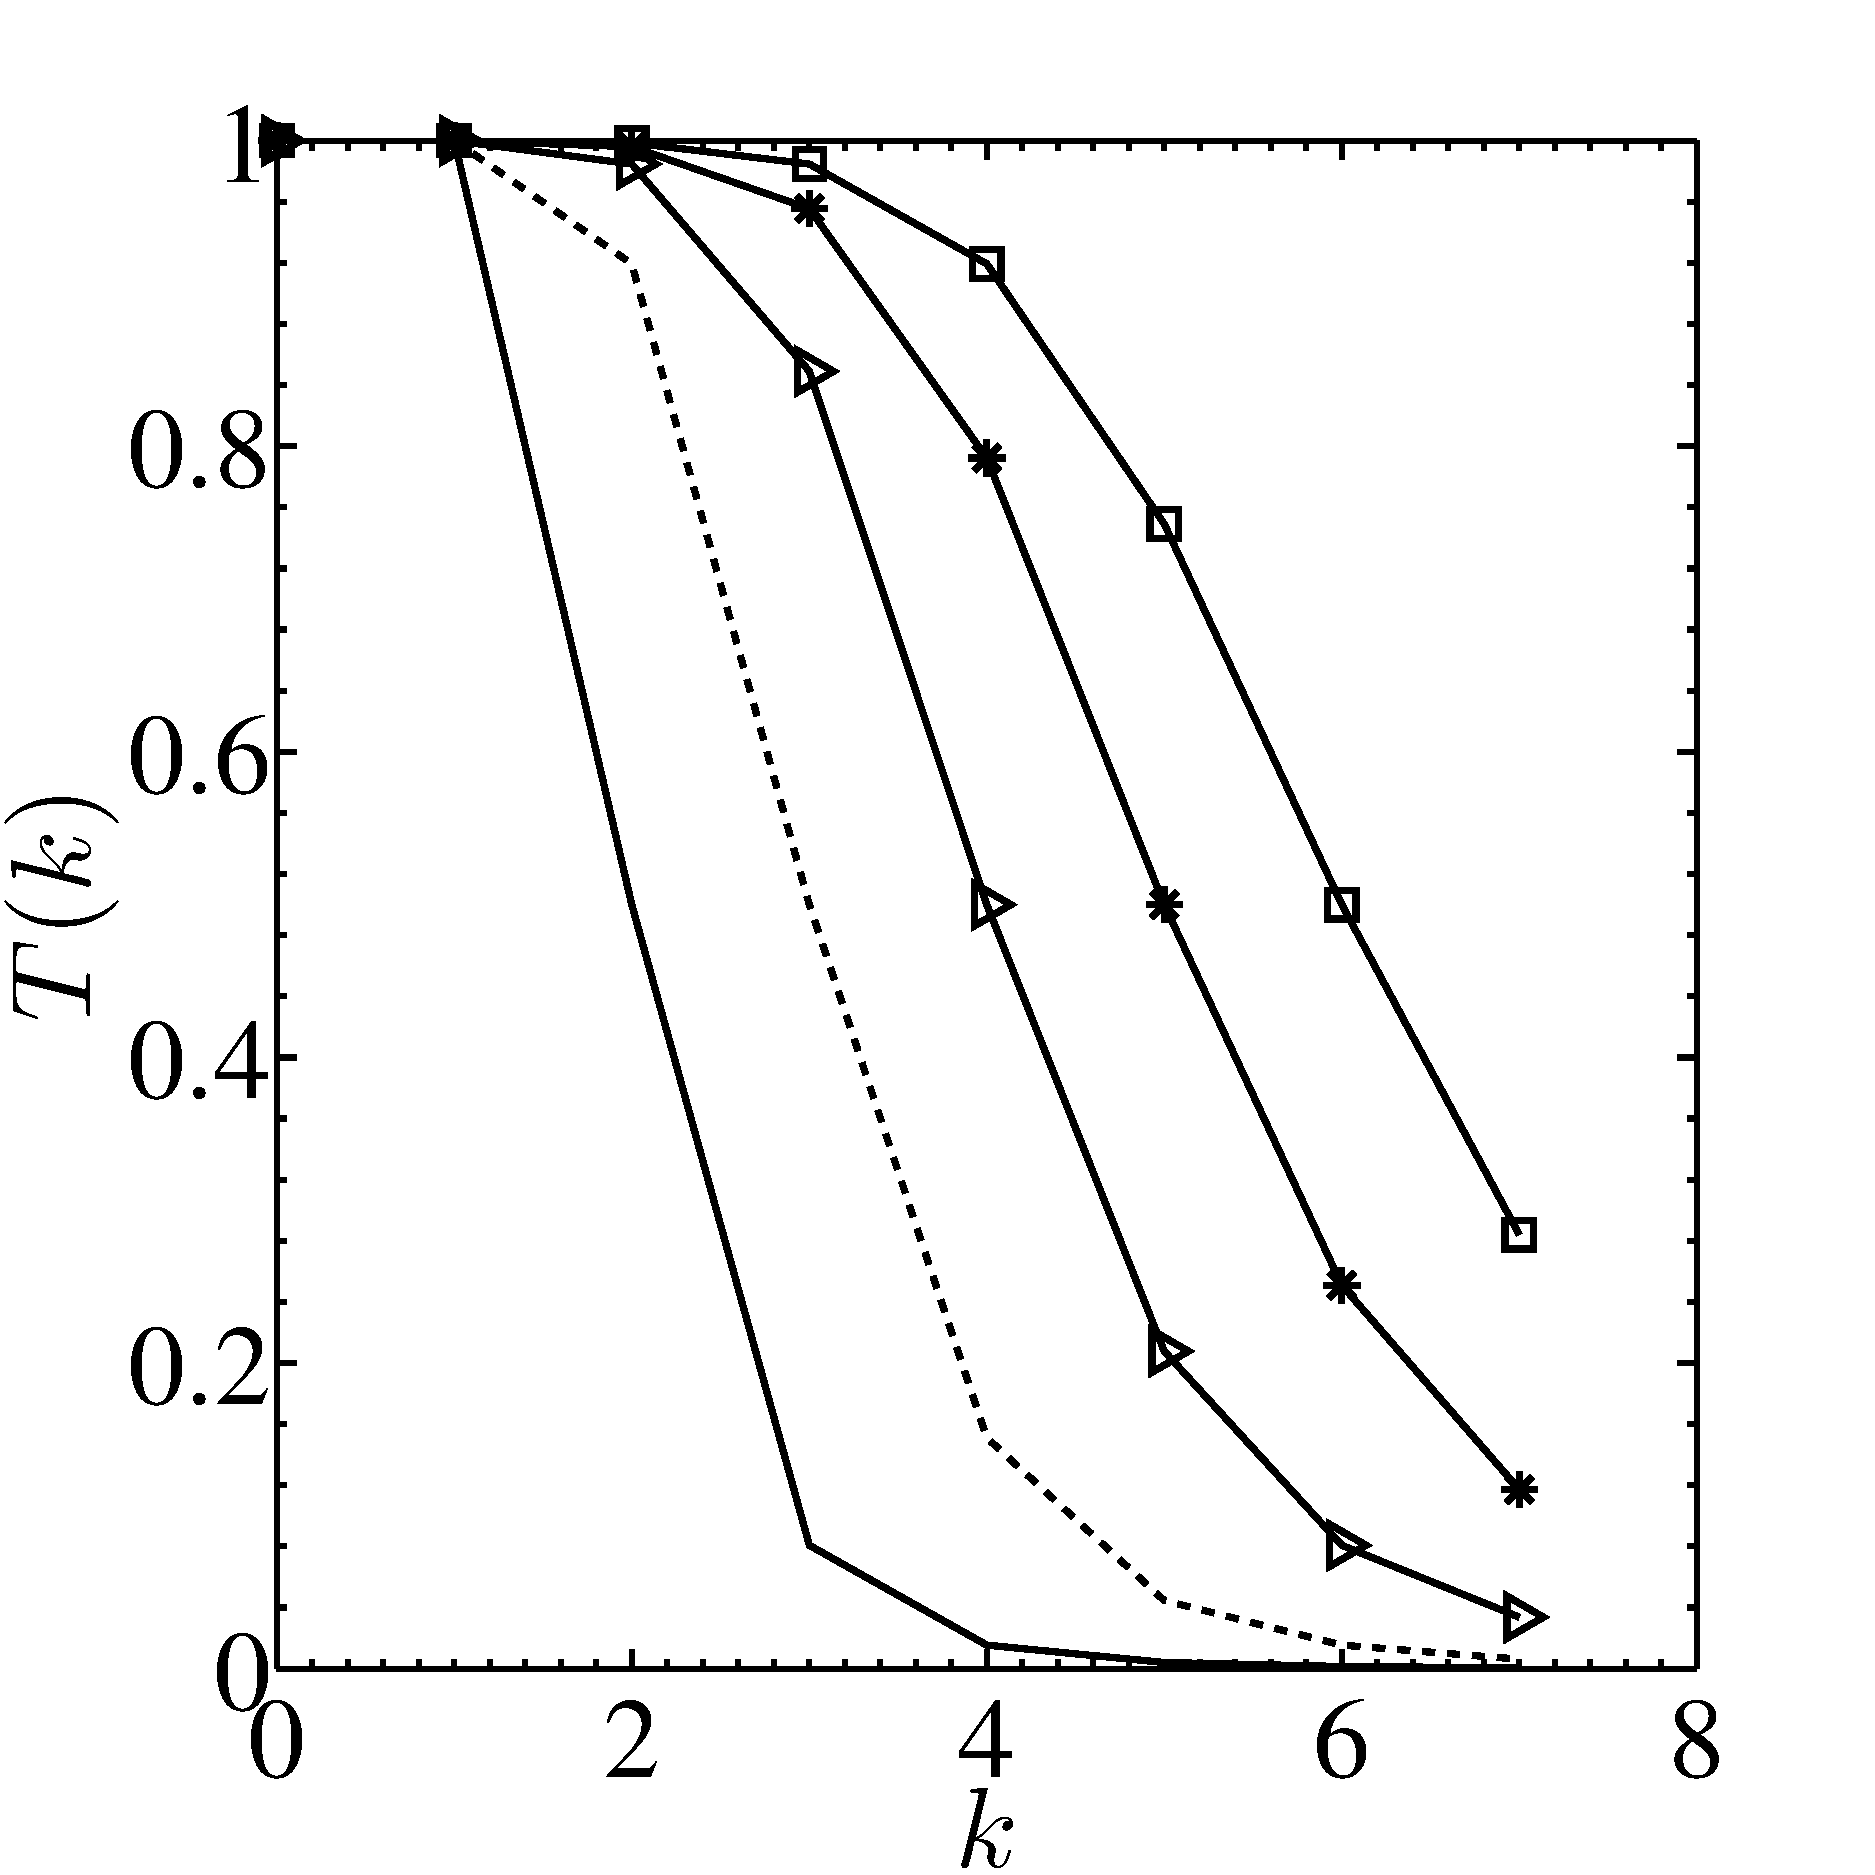
\includegraphics[width=\linewidth]{Figure/filter2.pdf}
                 \caption{}
                 \label{fig:filt2}
         \end{subfigure}%
         \begin{subfigure}[b]{0.32\textwidth}
         \centering
                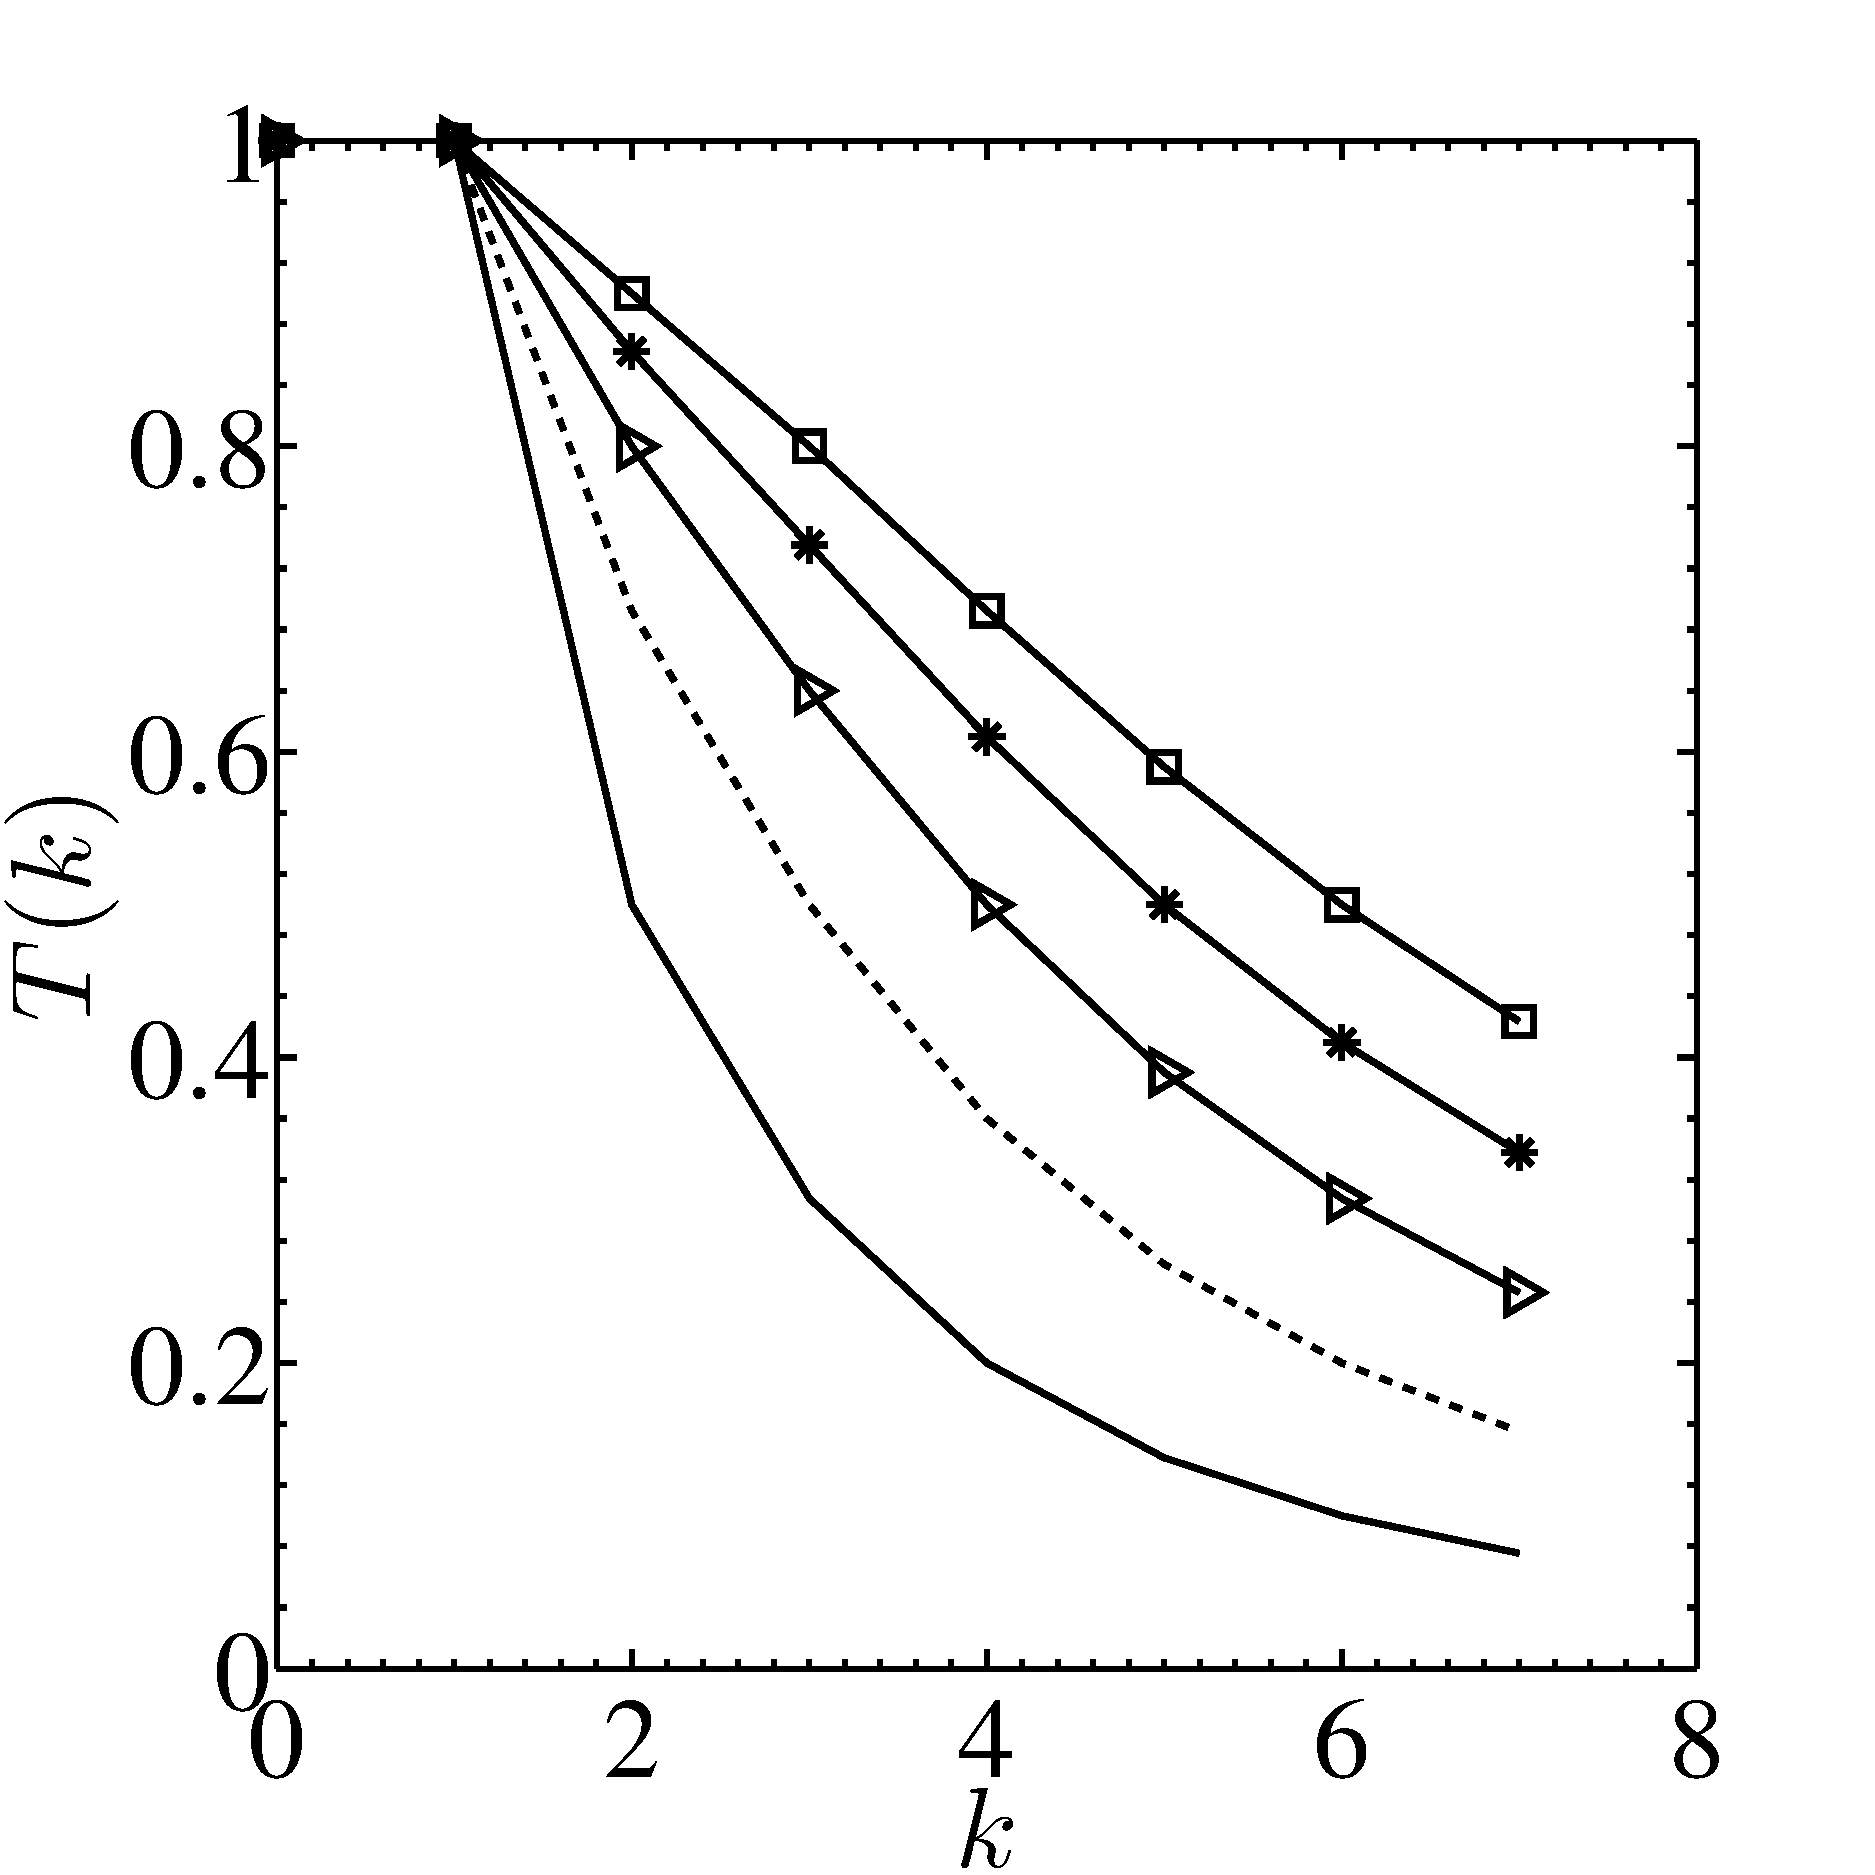
\includegraphics[width=\linewidth]{Figure/filter3.pdf}
                 \caption{}
                 \label{fig:filt3}
         \end{subfigure}
        \caption{Filter transfer function ${T}(k) = (1 + (k/k_{c})^\gamma)^{-1}$ (a) $\gamma = 12$ (b) $\gamma = 6$ (c) $\gamma = 2$.\hspace{2mm} $-$, $k_c = 2$; $--$, $k_c = 3$; $-.-$ $k_c = 4$; $-\star$, $k_c = 5$; $- \Box$ $k_c = 6$ $|$ ${T}(k_c) = \frac{1}{2}$. The total number of modes $k_{max} = N =7$, corresponding to GLL nodes = 8 (used in our simulation)}\label{fig:elem_filter}
\end{figure}

The low-pass filtering is performed in the modal space through a diagonal matrix $\mathbb{T}$ whose components are $T_0 = T_1 = 1$ (satisfying $C_0$ inter-element continuity) and $T_k = f(k;k_c) , \ \ \ 2\le k\le N$. $f(k;k_c$) is an attenuation function with increasing higher mode $k$, and $k_c$ is the cut-off value such that $T_k|_{k=k_c} = 1/2$ (See Figure~\ref{fig:elem_filter}). The filtering process in one dimension is given by
\begin{equation}
\widetilde{\mathbf{u}} = \mathcal{G}*\mathbf{u} = \Phi\mathbb{T}\Phi^{-1}\mathbf{u}.
\end{equation}
Extrapolation to 3D field can be achieved from 1D filter by a fast tensor product application~\cite{lynch}. 

The filtering attenuation function is given by
\begin{equation}
T_k = \frac{1}{1 + (k/k_c)^{\gamma}}, \ \ \ \ 2\le k\le N.\label{eq:Tk}
\end{equation}
Both parameters in Equation~(\ref{eq:Tk}), $k_c$ and $\gamma$, determine the precise shape of the filter transfer function. It is observed that decreasing $k_c$ quite straightforwardly attenuate the large scale contents of the filtered velocity $\widetilde{u}_{i}$, while decreasing $\gamma$ smoothens the transfer function more towards non-projective filtering as seen in Figure~\ref{fig:filt1},~\ref{fig:filt2},~\ref{fig:filt3}. 

\par
\section{Results and Discussion}\label{results}
In this section, the LES simulation results for different parametric tests have been presented and benchmarked with the past literature with a rigorous analysis on the observed results in order to comment on the robustness of the model. To start with, we present the results of mean statistics for different values of the filter cut-off wave-numbers $k_{c}$ (See Section~\ref{element_level}) using mid-point interpolation for approximate stress boundary condition which can be given as $\widehat{\widetilde{u}}_{i,r,\frac{\Delta z}{2}} = \frac{1}{2} (\widehat{\widetilde{u}}_{i,r}(x,y,0,t) + \widehat{\widetilde{u}}_{i,r}(x,y,\Delta z,t))$ (Refer to Section~\ref{nwm}). The logarithmic trends of the nondimensional streamwise velocity profile ${U}/{u_{\tau}}$ and the non-dimensional mean streamwise velocity gradient $\Phi = \frac{\kappa z}{u_{\tau}}dU/dz$ are shown in Figure~\ref{fig:velocity},~\ref{fig:gradient}. Velocity $U$ is the temporal and horizontally averaged (homogeneous $x-y$ plane) mean velocity profile $\langle\widetilde{u}_{i}\rangle_{xy}$. All the plots involving physical length scale $z$ has been normalized with the boundary layer thickness $H$. From the trends of the velocity profile, we observe that explicit filtering with $k_c = 2, \  \gamma = 12$ shows overall better match of the logarithmic trend as opposed to $k_c = 1, 4$. Even though ~\cite{porte1fun} reports a strong deviation of the logarithmic profile from around $z/H \sim 0.3$ into the so called ``wake" region, our current simulation still maintains a logarithmic trend at  $z/H \sim 0.3--0.4$, and small deviation into the wake region. It is interesting to note, that in the near wall region ($z/H \lessapprox 0.1$) filtering with $k_c = 4$ shows a reasonable match with the scale dependant model~\cite{porte1fun}, while $k_c = 2$ shows consistency with the near wall region of standard Smagorinsky model~\cite{porte1fun}. This is further corroborated in the plot of mean velocity gradients (See Figure~\ref{fig:gradient}), which shows comparison against the results of Porte-Agel~\cite{porte1fun} and Bou-Zeid~\cite{bou1}. The plots of normalized gradient shows that explicit filtering with $k_c = 1, \ 2, \ 4$, remains closest to 1, predicting log-law of the wall. However, the slope decrease to $~0.8$ for $k_c = 1$. So in terms of gradient, it can be seen that none of the literatures~\cite{porte1fun,bou1} predict exact value of 1 in the near-wall region which justifies that with explicit filtering of $k_c = 2, 4$ is in a good concordance with results of the literature~\cite{porte1fun,bou1}. The plot in the inset of Figure~\ref{fig:gradient} shoots quite sharply to zero at $z/H = 1$ which manifests the stress-free boundary conditions at the top of ABL. \\
\par
  Figure~\ref{fig:stat2} shows comparison of the resolved second-order statistics of velocity fields $\widetilde{{u'}_{i}{u'}_{j}}$, where $\widetilde{u'}_{i} = \widetilde{u}_{i} - \langle\widetilde{u}_{i}\rangle_{xy} $, ($rms$ and kinematic shear stress) non-dimensionalized with $u_{\tau}^{2}$. The plots of $u_{rms}$, $v_{rms}$, $w_{rms}$ shows slight discrepancies in the statistics in the upper region of the boundary layer at $z/H \gtrapprox 0.5$. Statistics $u_{rms}$  matches the scale-dpendant model~\cite{porte1fun} reasonably well in the region of $z/H \sim 0.1 - 0.4$ especially for explicit filtering $k_c = 4$. Statistics $v_{rms}$ is in excellent agreement with the standard Smagorinsky model~\cite{porte1fun} for all $k_{c}$, but shows deviation in the extreme upper region and near-wall region for scale dependant model. This can be attributed to vulnerability of $v_{rms}$ to wall damping in spectral methods. The statistic $w_{rms}$ shows quite a good match with the standard Smagorinsky model all the way except in the near wall region $z/H \sim 0.1$ , where it shows a good match with the scale-dependant model (scale-dependant model~\cite{porte1fun} decreases the peak of $w_{rms}$ and increases the peak of $v_{rms}$ in the near-wall region as compared to standard Smagorinsky model). We make a careful analysis of the kinematic shear stress $uw_{rms}$ in Figure~\ref{fig:uwrms}. With $Re \sim 10^{10}$, eddy-viscosity in the current LES model results in $\nu_{t} \gg \nu \approx 0$ which indicates the kinematic shear stress in an LES framework for a flat-plate type geometry can be given as
  \begin{align*}
-{\widetilde{u'_{1}u'_{3}}} + \nu_{t}\frac{\partial U}{\partial z} \approx \tau_{w}(1 - \frac{z}{H}) 
\end{align*}
 We see in the near-wall region, the subgrid stress $\nu_{t}\frac{\partial U}{\partial z}$ dominates, which deviates the shear stress $\widetilde{u'_{1}u'_{3}} = uw_{rms}$ significantly away from the linear slope, while far away from the wall, a linear trend of the kinematic shear stress is expected. We observe that in Figure~\ref{fig:uwrms}, the explicit filtering $k_c = 4$ and even $k_c = 2$ to a significant extent follows the linear trend in the shear stress expected from a DNS, before deviating due to the near wall damping by eddy-viscosity model at around $z/H \sim 0.1$. We observe that with filtering $k_c = 1$, there is over prediction of shear stress in the middle of the boundary layer (bulges), while all the models of Port$\acute{e}$-Agel et al. starts showing attenuation of the shear stress and deviation from the linear trends from the upper-region of boundary layer. The deviation observed, is more intense in the case of scale-dependant model, even though we observe a very good match of the peak location and the shear stress in the extreme near wall region ($z/H \lessapprox 0.1$).\\
\par
Next, we present the streamwise kinetic energy spectra of the turbulent velocity field. The streamwise kinetic energy spectra has been normalized with $u_\tau^{2} z$, where $z$ is the height at which the horizontal slices are taken and the streamwise wavenumber $k_{1}$ has been scaled with $z$ for non-dimensionalization. The results have been compared against the data of Port$\acute{e}$-Agel et al.~\cite{porte1fun}. It is intriguing to notice, that the current spectrum plots reproduce the $k_{1}^{-1}$ and $k_{1}^{-5/3}$ quite faithfully as documented in the previous literatures~\cite{kader,katul}. The present plots depict the streamwise spectrum at further away from the near wall region, than has been reported in the literature. With the current normalization, it is observed, that the $5/3$ law region collapse as expected ~\cite{katul,porte1fun}, but the present simulations depict the $k_{1}^{-1}$ region far more faithfully at $k_{1}z \lessapprox 1$ than~\cite{porte1fun} which shows deviation to slopes $\sim k_{1}^{-1.5} -k_{1}^{-2}$ as we increase $z/H$ .i.e., towards the core of the boundary layer. It is further observed that the dissipation of the streamwise energy spectrum occurs at increasing $k_{1}z$ as we move from the near wall region to the upper region of the boundary layer which are also reported in the literature~\cite{kader,katul,porte1fun,bou1}.
\begin{figure}
\centering
        \begin{subfigure}[t]{0.55\textwidth}
                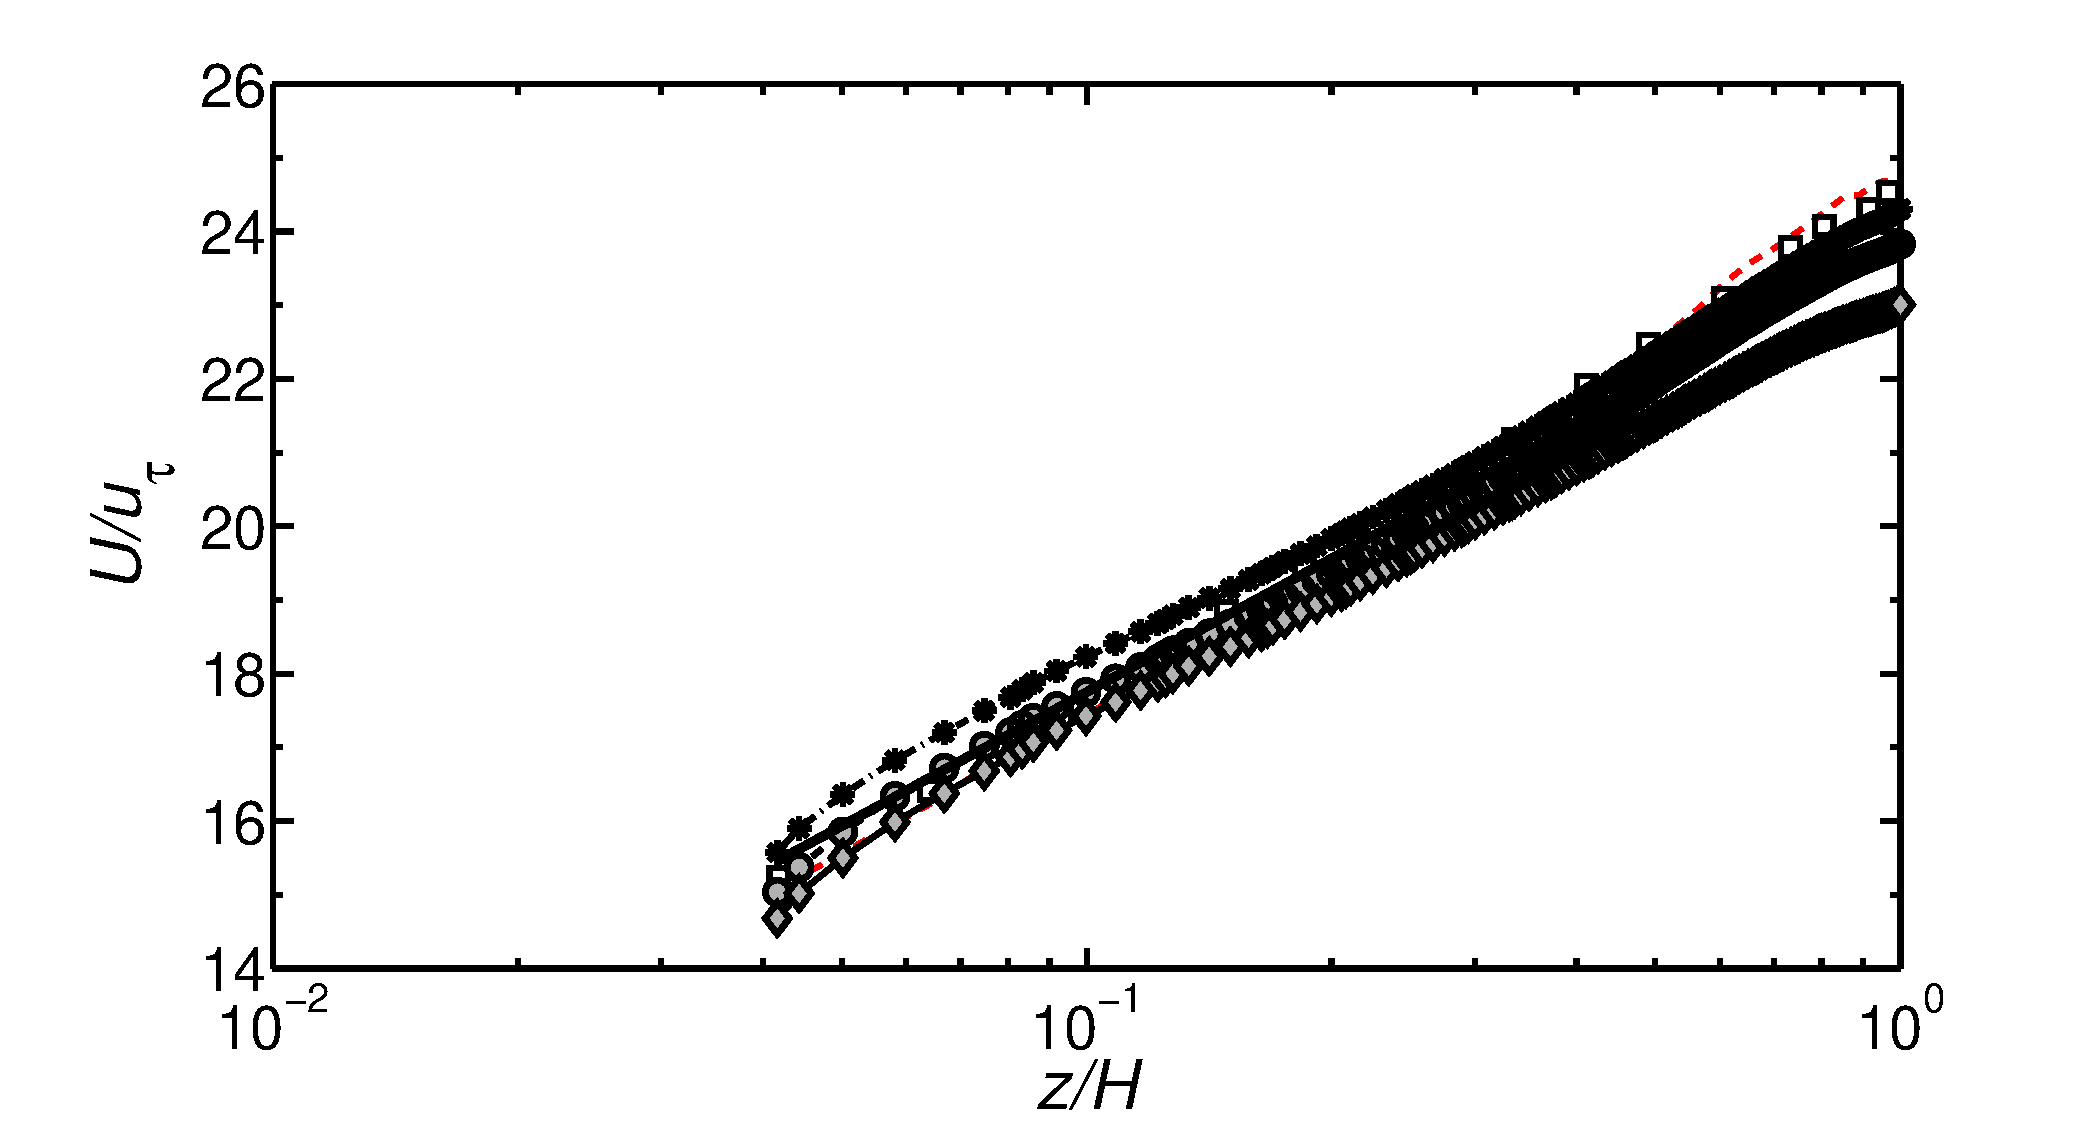
\includegraphics[width=\linewidth]{Fig3/velcomp_filter_paper.pdf}
                \caption{}
                \label{fig:velocity}
        \end{subfigure}%
        \centering
        \begin{subfigure}[t]{0.45\textwidth}
                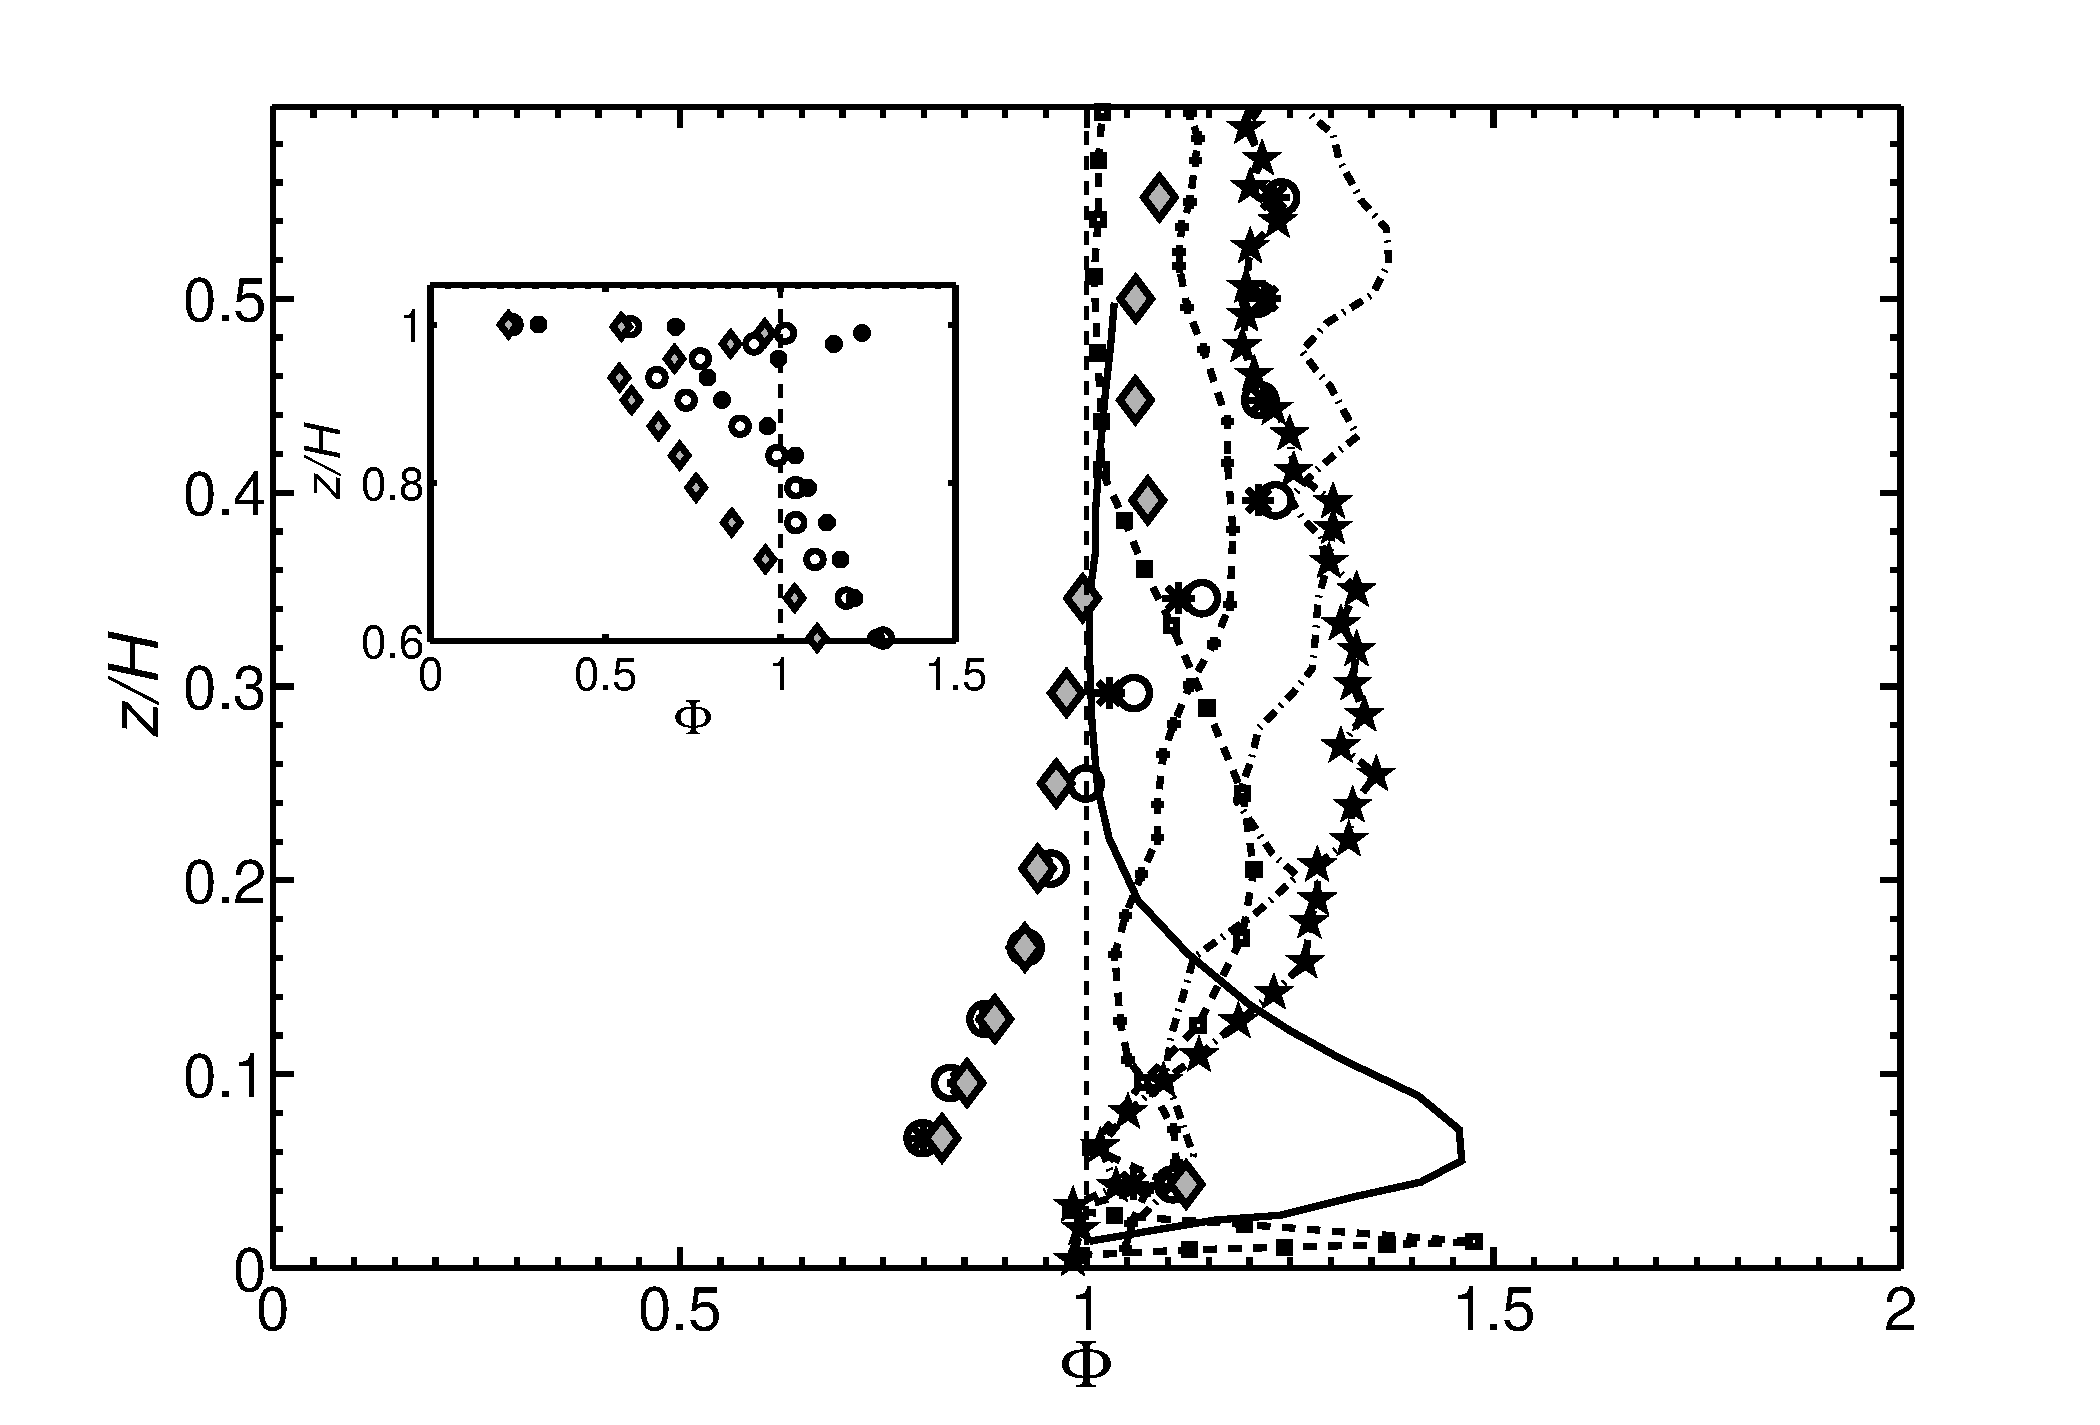
\includegraphics[width=\linewidth]{Fig3/gradient_filt.pdf}
                \caption{}
                \label{fig:gradient}
        \end{subfigure}
        \caption{logarithmic trends of mean velocity profile in ABL simulations at $Re = 10^{10}$ using mid-point interpolation. (a) grey $\circ$, $k_{c}=2$; black $\star$, $k_{c}=1$; gray $\diamond$, $k_{c}=4$, ($\gamma = 12\ \forall k_c$ ) for current simulation (SEM) using standard Smagorinsky ($C_s = 0.15, n = 2$); $-+$ black, standard Smagorinsky ($C_s = 0.15, n = 2$) and black $\Box$ scale dependant dynamic Smagorinsky for Port$\acute{e}$-Agel et al.~\cite{porte1fun}; $-$ black, a least-squares fit. Expected logarithmic trend in lower $10-20 \%$ of the boundary layer ($z/H \sim 0.1$). $k_{c}$ is the number of Legendre polynomial modes in the explicit filtering of wall BC. (b) Mean velocity gradient $\Phi = \frac{\kappa z}{u_{\tau}}\frac{d \overline{U}}{dZ}$ variation over $z/H$.  white $\circ$, $k_{c}=2$; gray $\diamond$, $k_{c}=1$; black $*$, $k_{c}=4$ for present simulation (SEM); black $--\star$, standard Smagorinsky ($C_s = 0.15, n = 2$); black $-.$, scale dependant dynamic Smagorinsky for Port$\acute{e}$-Agel et al.~\cite{porte1fun}; lagrangian scale dependant dynamic Smagorinsky model, black $-\square$, without filtering; black $-\star$ with filtering, Bou-Zeid et al.~\cite{bou1}  }\label{fig:stat}
\end{figure}

\begin{figure}
\centering
        \begin{subfigure}[t]{0.29\textwidth}
                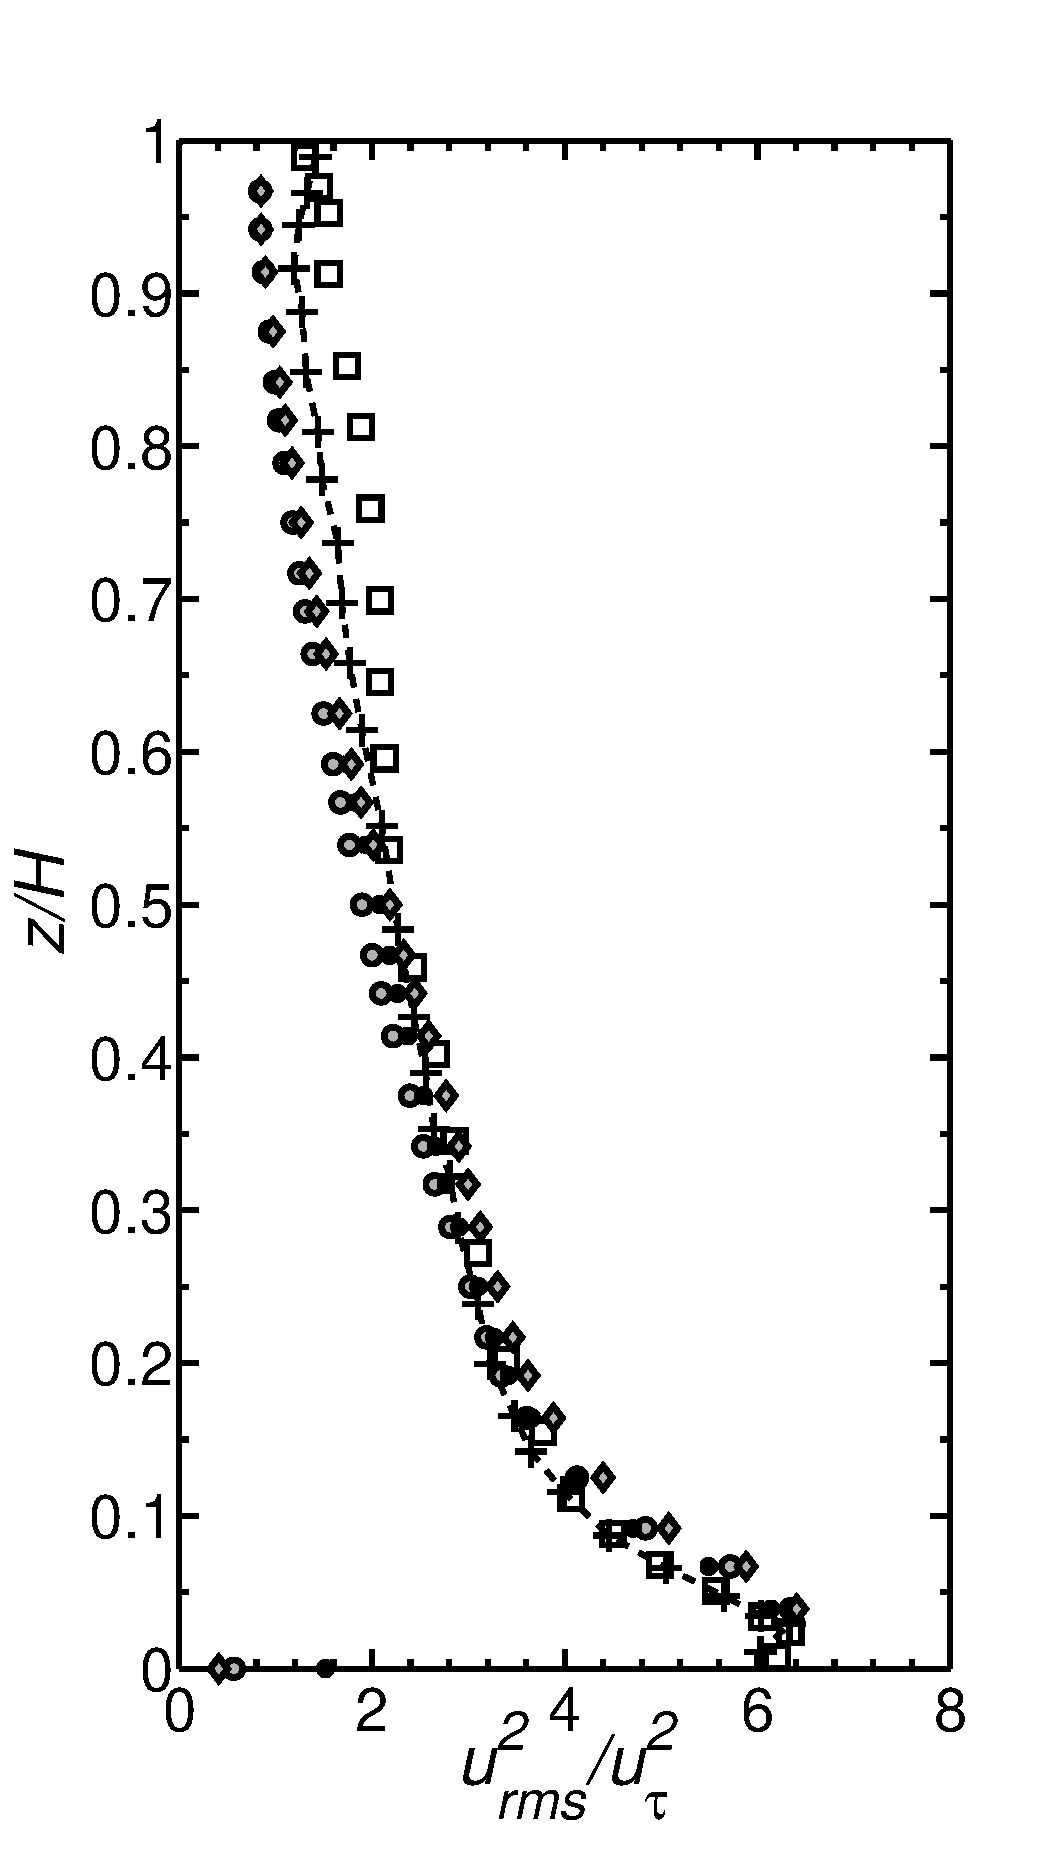
\includegraphics[width=\linewidth]{Fig3/urms_filter_paper.pdf}
                \caption{}
                \label{fig:urms}
        \end{subfigure}%
        \centering
        \begin{subfigure}[t]{0.29\textwidth}
                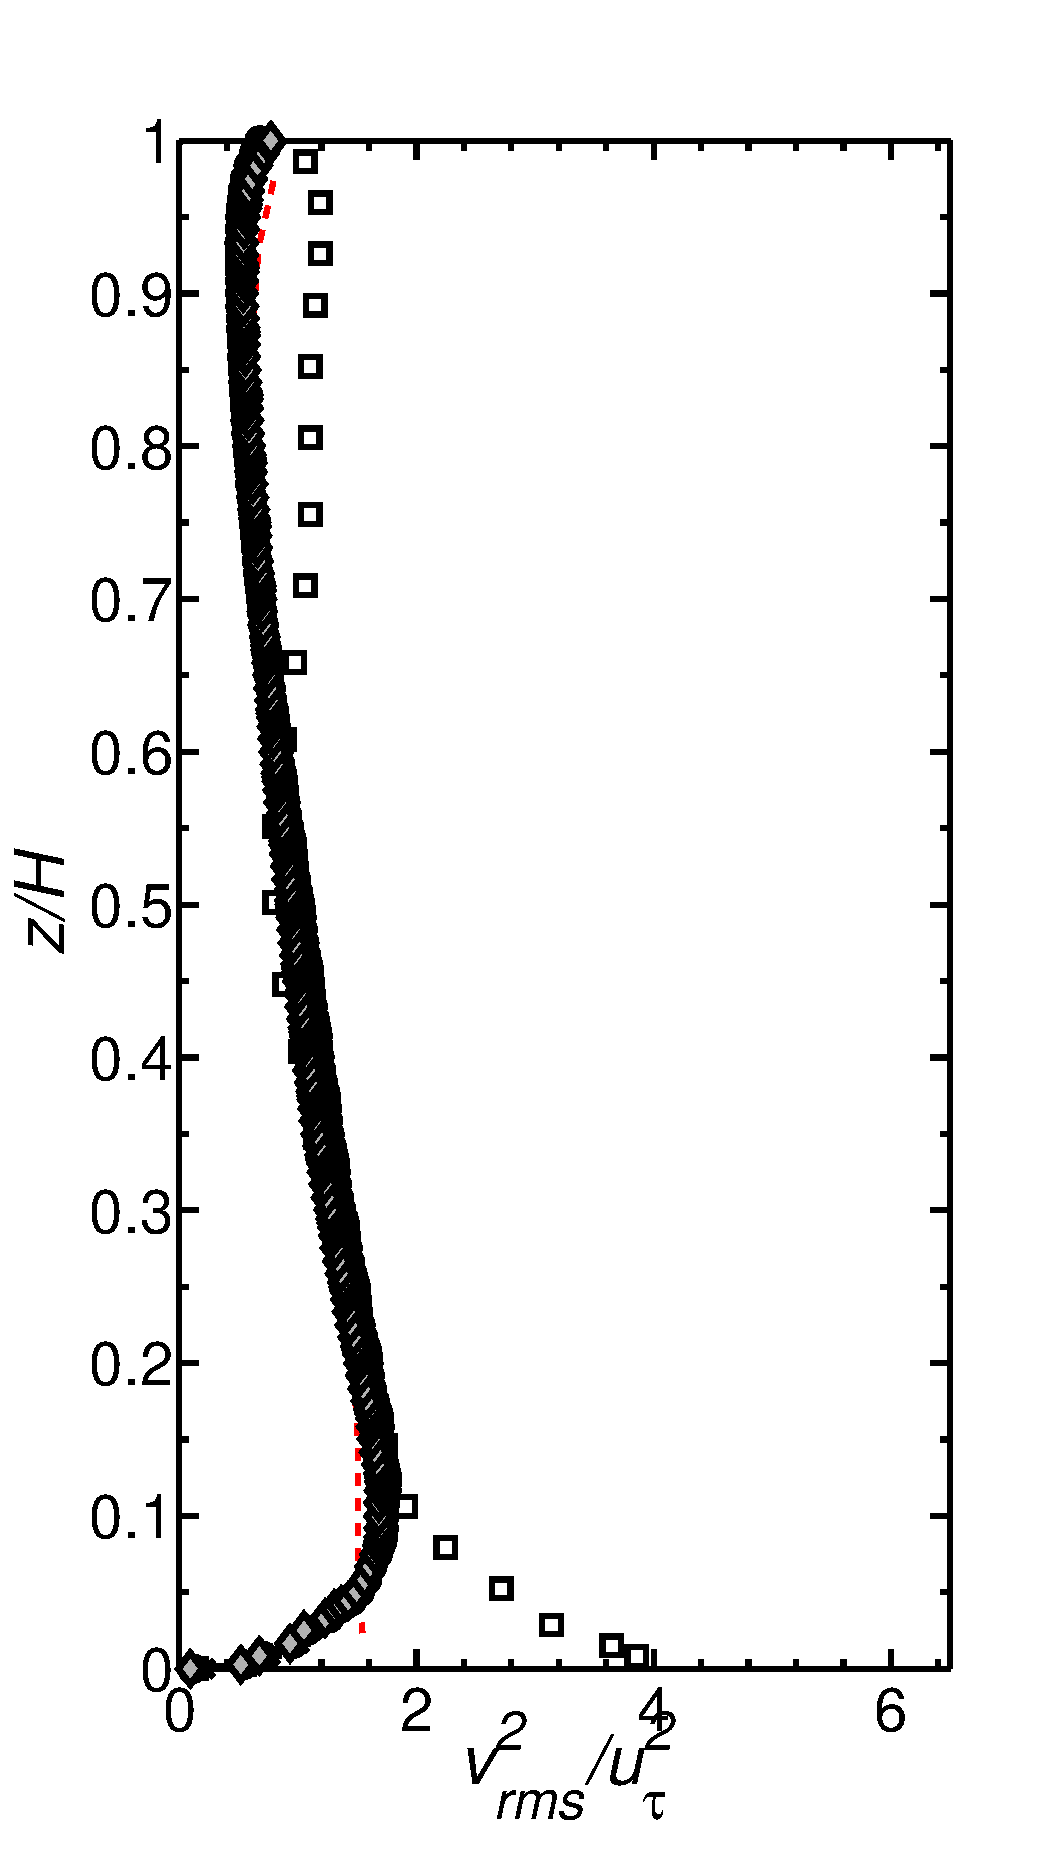
\includegraphics[width=\linewidth]{Fig3/vrms_filter_paper.pdf}
                \caption{}
                \label{fig:vrms}
        \end{subfigure}%
        \centering
        \begin{subfigure}[t]{0.29\textwidth}
                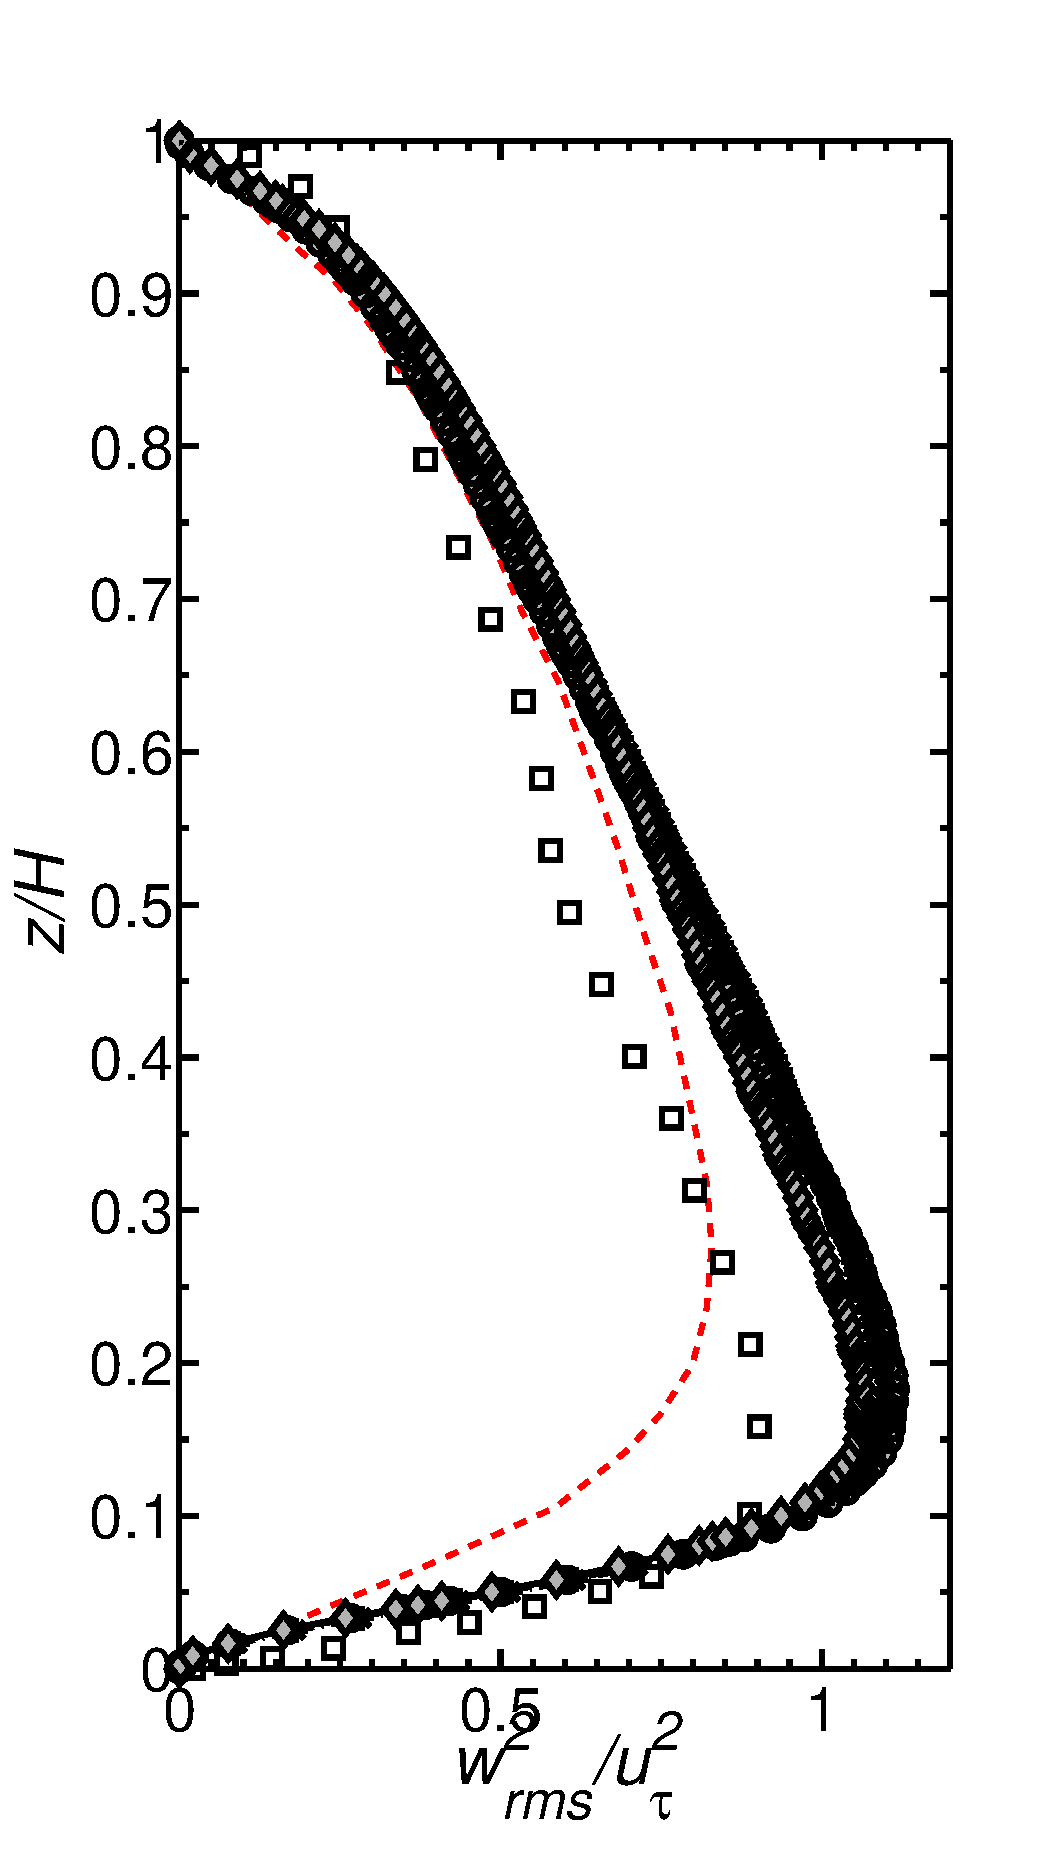
\includegraphics[width=\linewidth]{Fig3/wrms_filter_paper.pdf}
                \caption{}
                \label{fig:wrms}
        \end{subfigure}
        \centering
        \begin{subfigure}[t]{0.60\textwidth}
                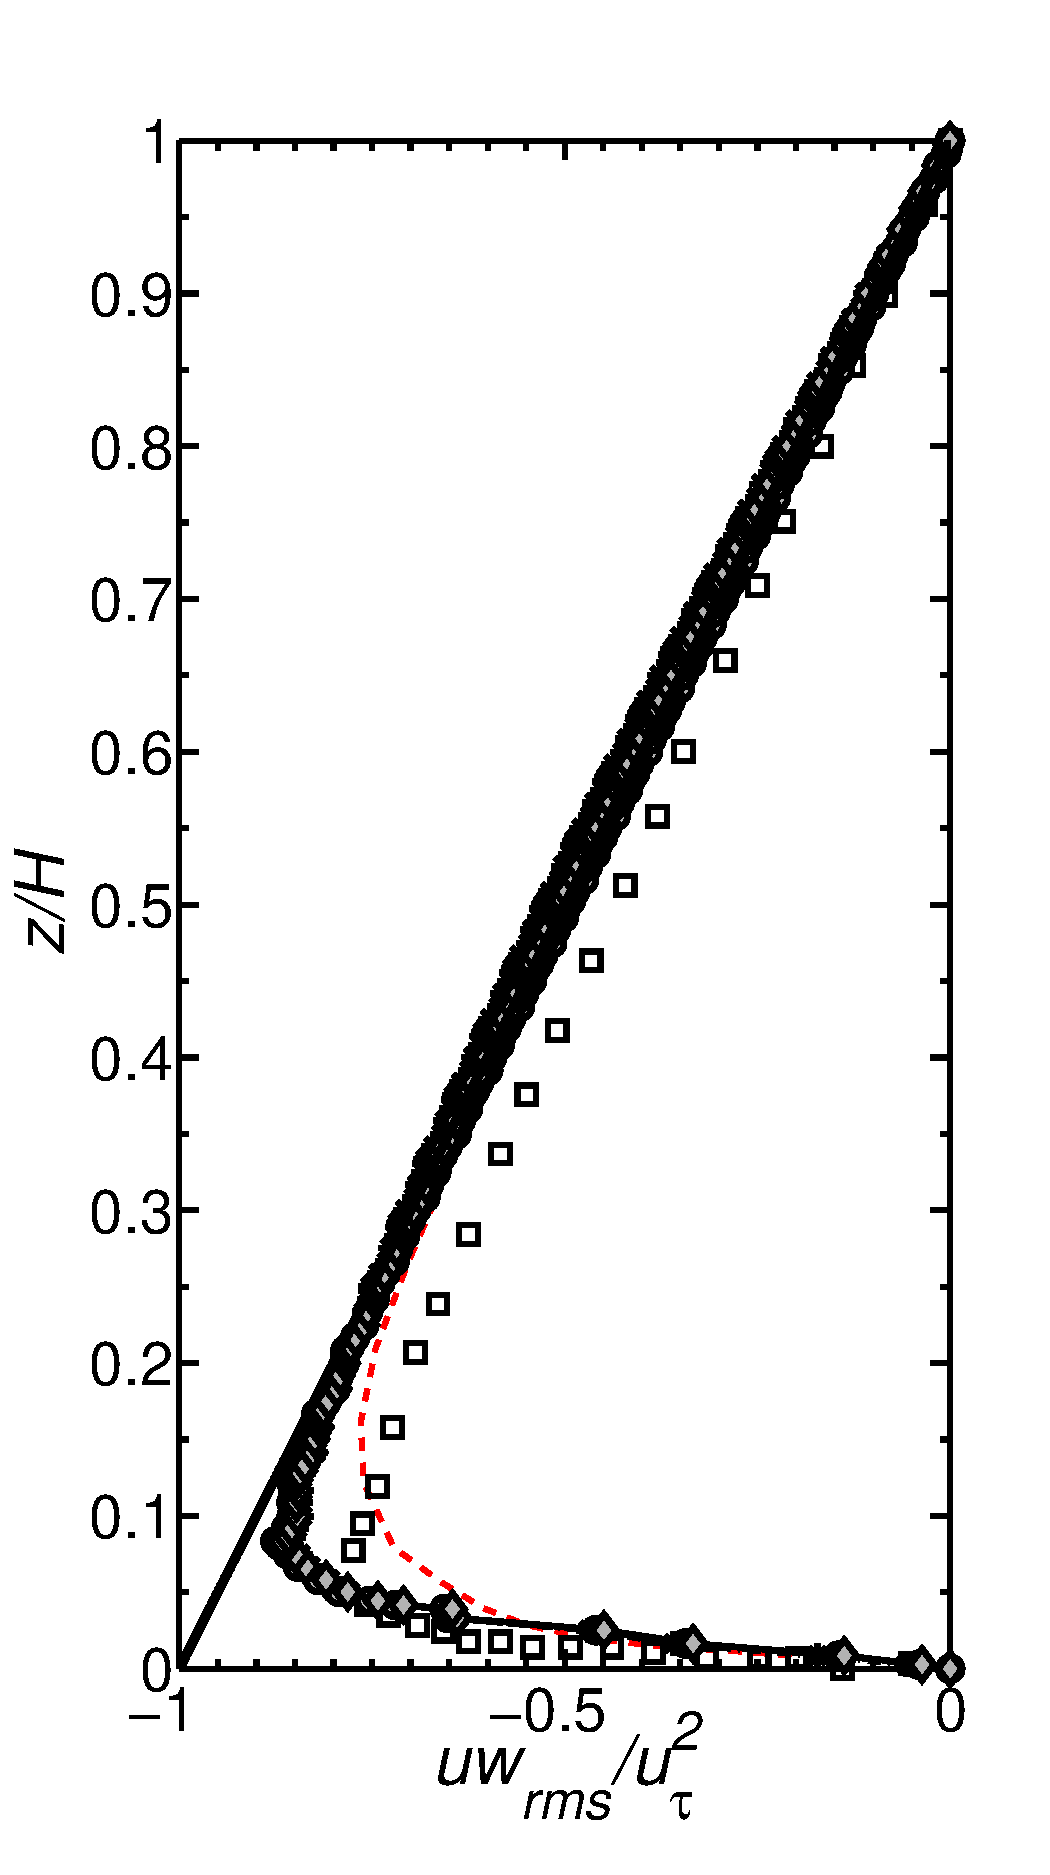
\includegraphics[width=\linewidth]{Fig3/uwrms_filter_paper.pdf}
                \caption{}
                \label{fig:uwrms}
        \end{subfigure}%
        \caption{Second order statistics for ABL simulations at $Re = 10^{10}$ using mid-point interpolation. (a) $u_{rms}$ (b) $v_{rms}$ (c) $w_{rms}$ (d) $uw_{rms}$. gray $\circ$, $k_{c}=2$; black $\star$, $k_{c}=1$; gray $\diamond$, $k_{c}=4$, for current simulation (SEM) using standard Smagorinsky ($C_s = 0.15, n = 2$); $-+$ black, standard Smagorinsky ($C_s = 0.15, n = 2$) and black $\Box$ scale dependant dynamic Smagorinsky for Port$\acute{e}$-Agel et al.~\cite{porte1fun}.}\label{fig:stat2}
\end{figure}


\begin{figure}
\centering
        \begin{subfigure}[t]{0.30\textwidth}
                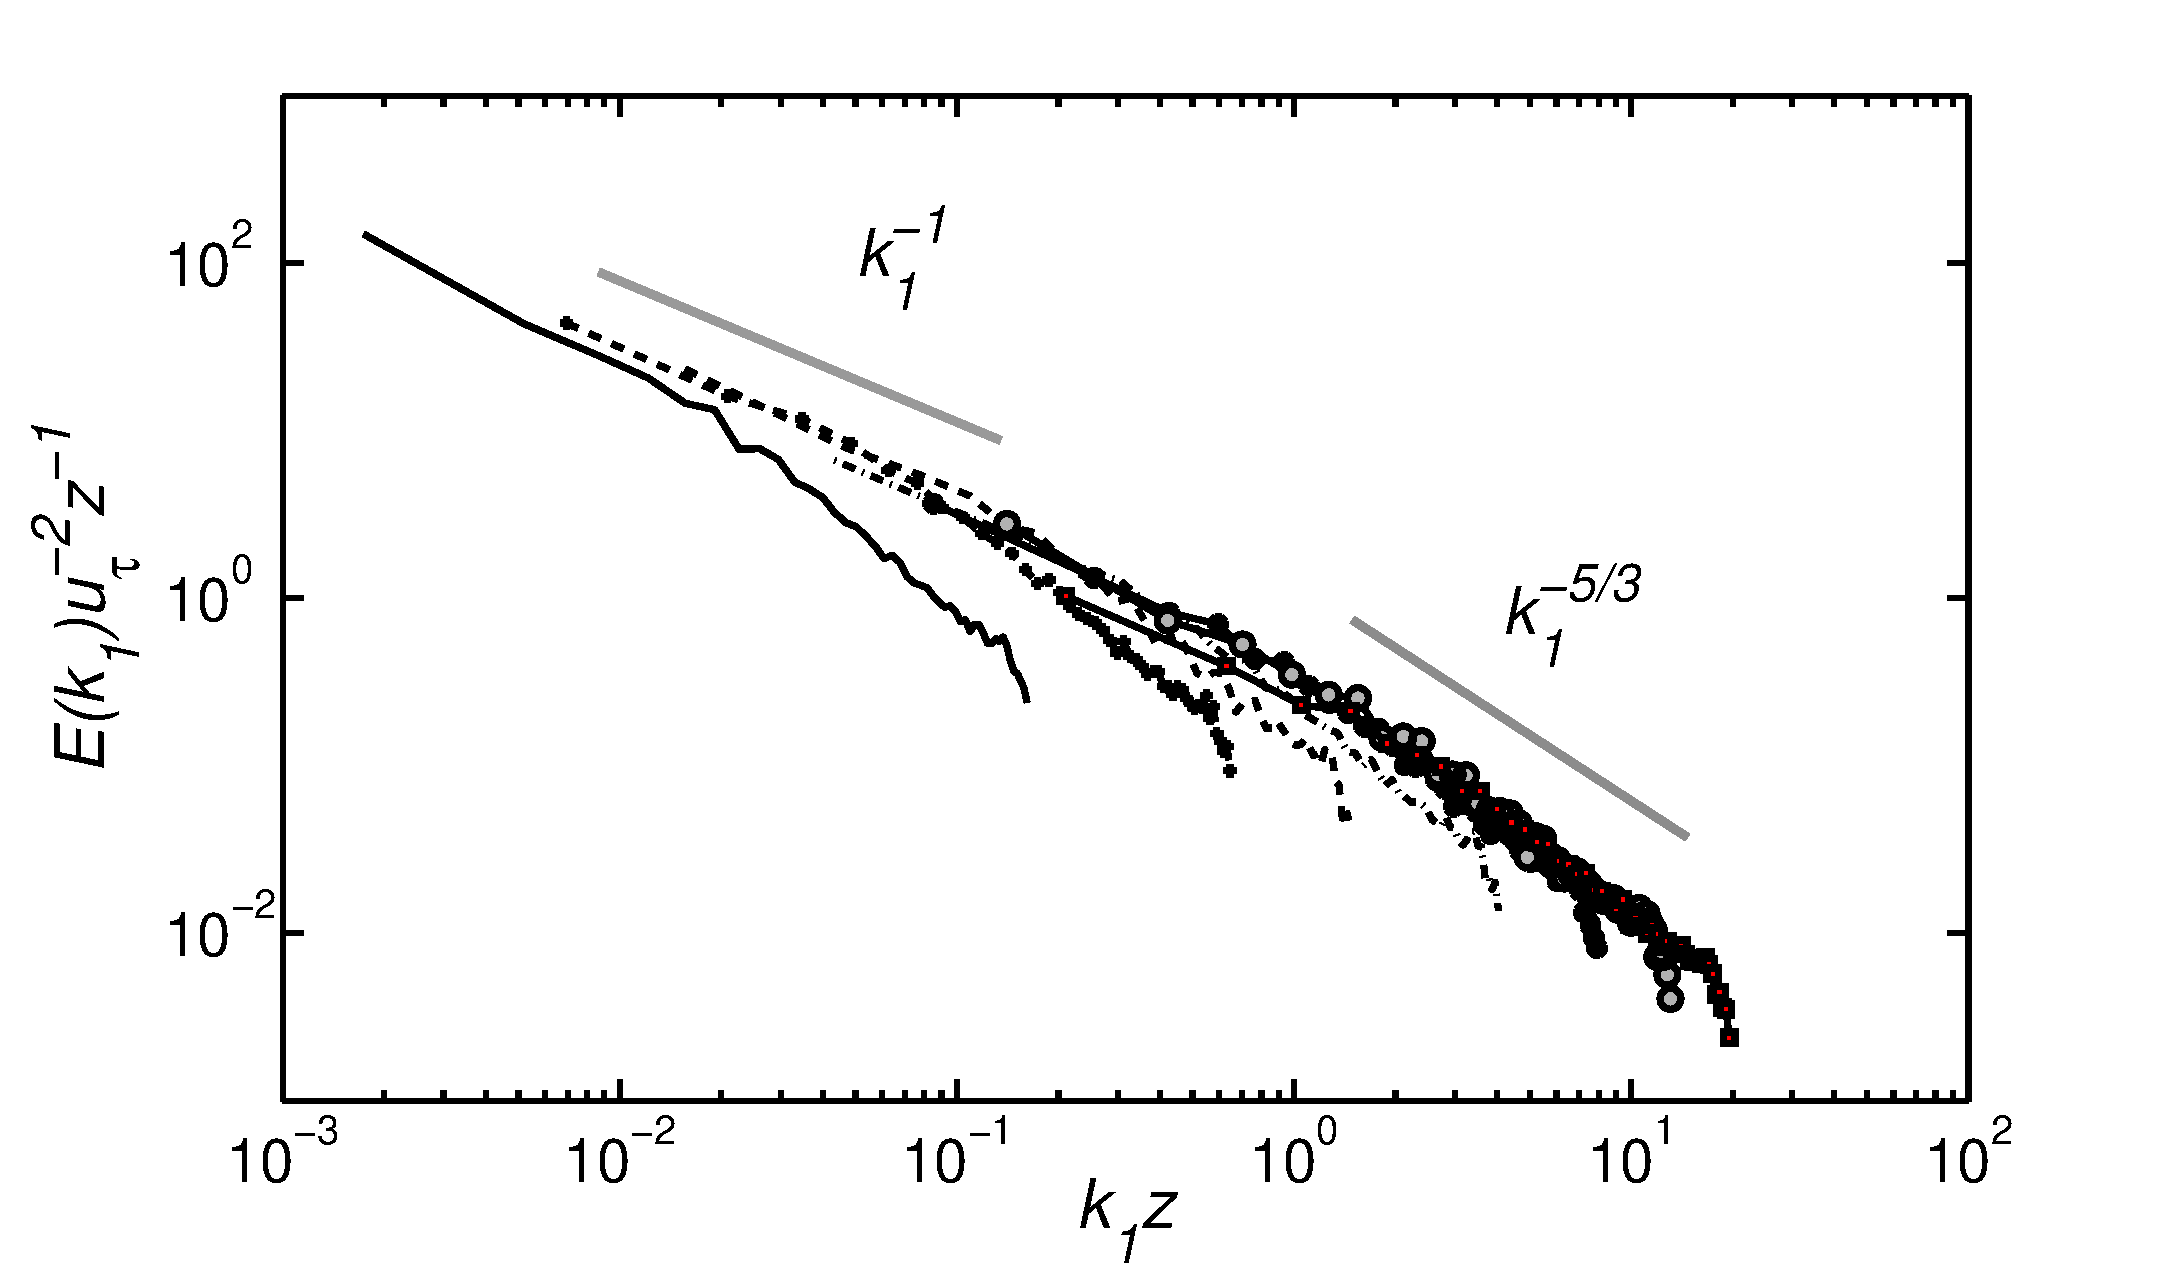
\includegraphics[width=\linewidth]{Figure/energy3.pdf}
                \caption{}
                \label{fig:eng1}
        \end{subfigure}%
        \centering
        \begin{subfigure}[t]{0.30\textwidth}
                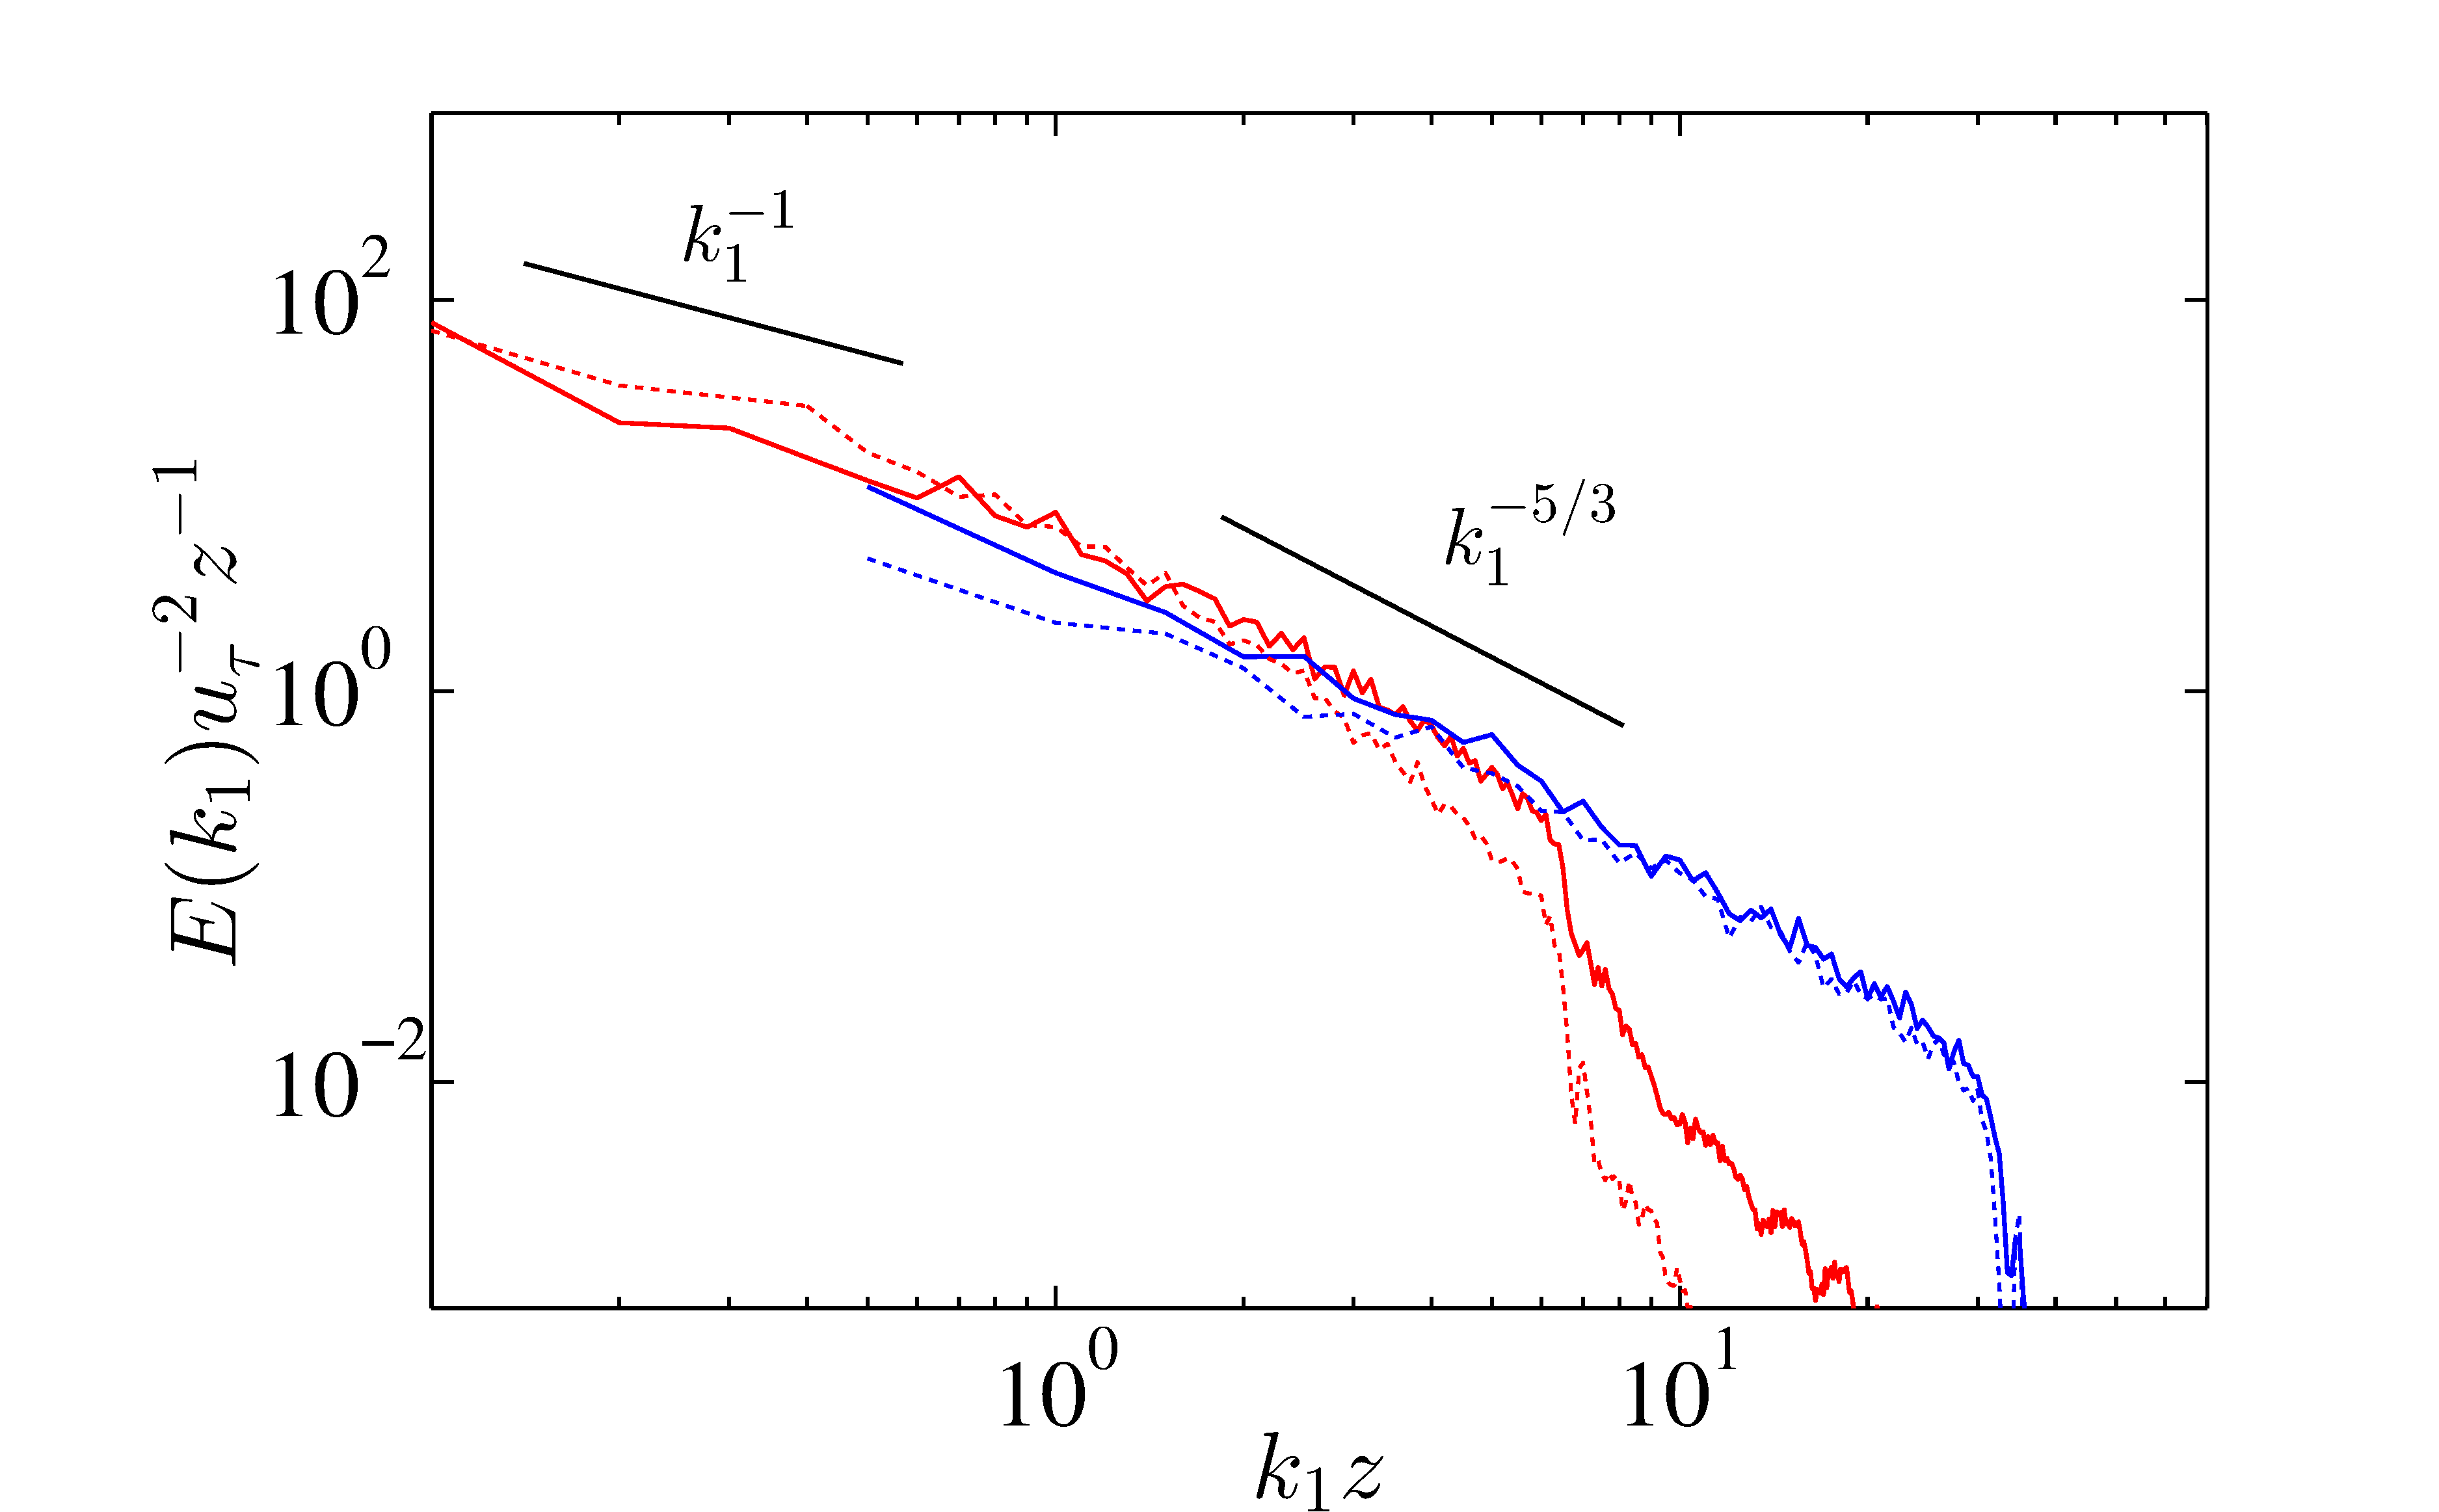
\includegraphics[width=\linewidth]{Figure/energy.pdf}
                \caption{}
                \label{fig:eng2}
        \end{subfigure}%
        \centering
        \begin{subfigure}[t]{0.30\textwidth}
                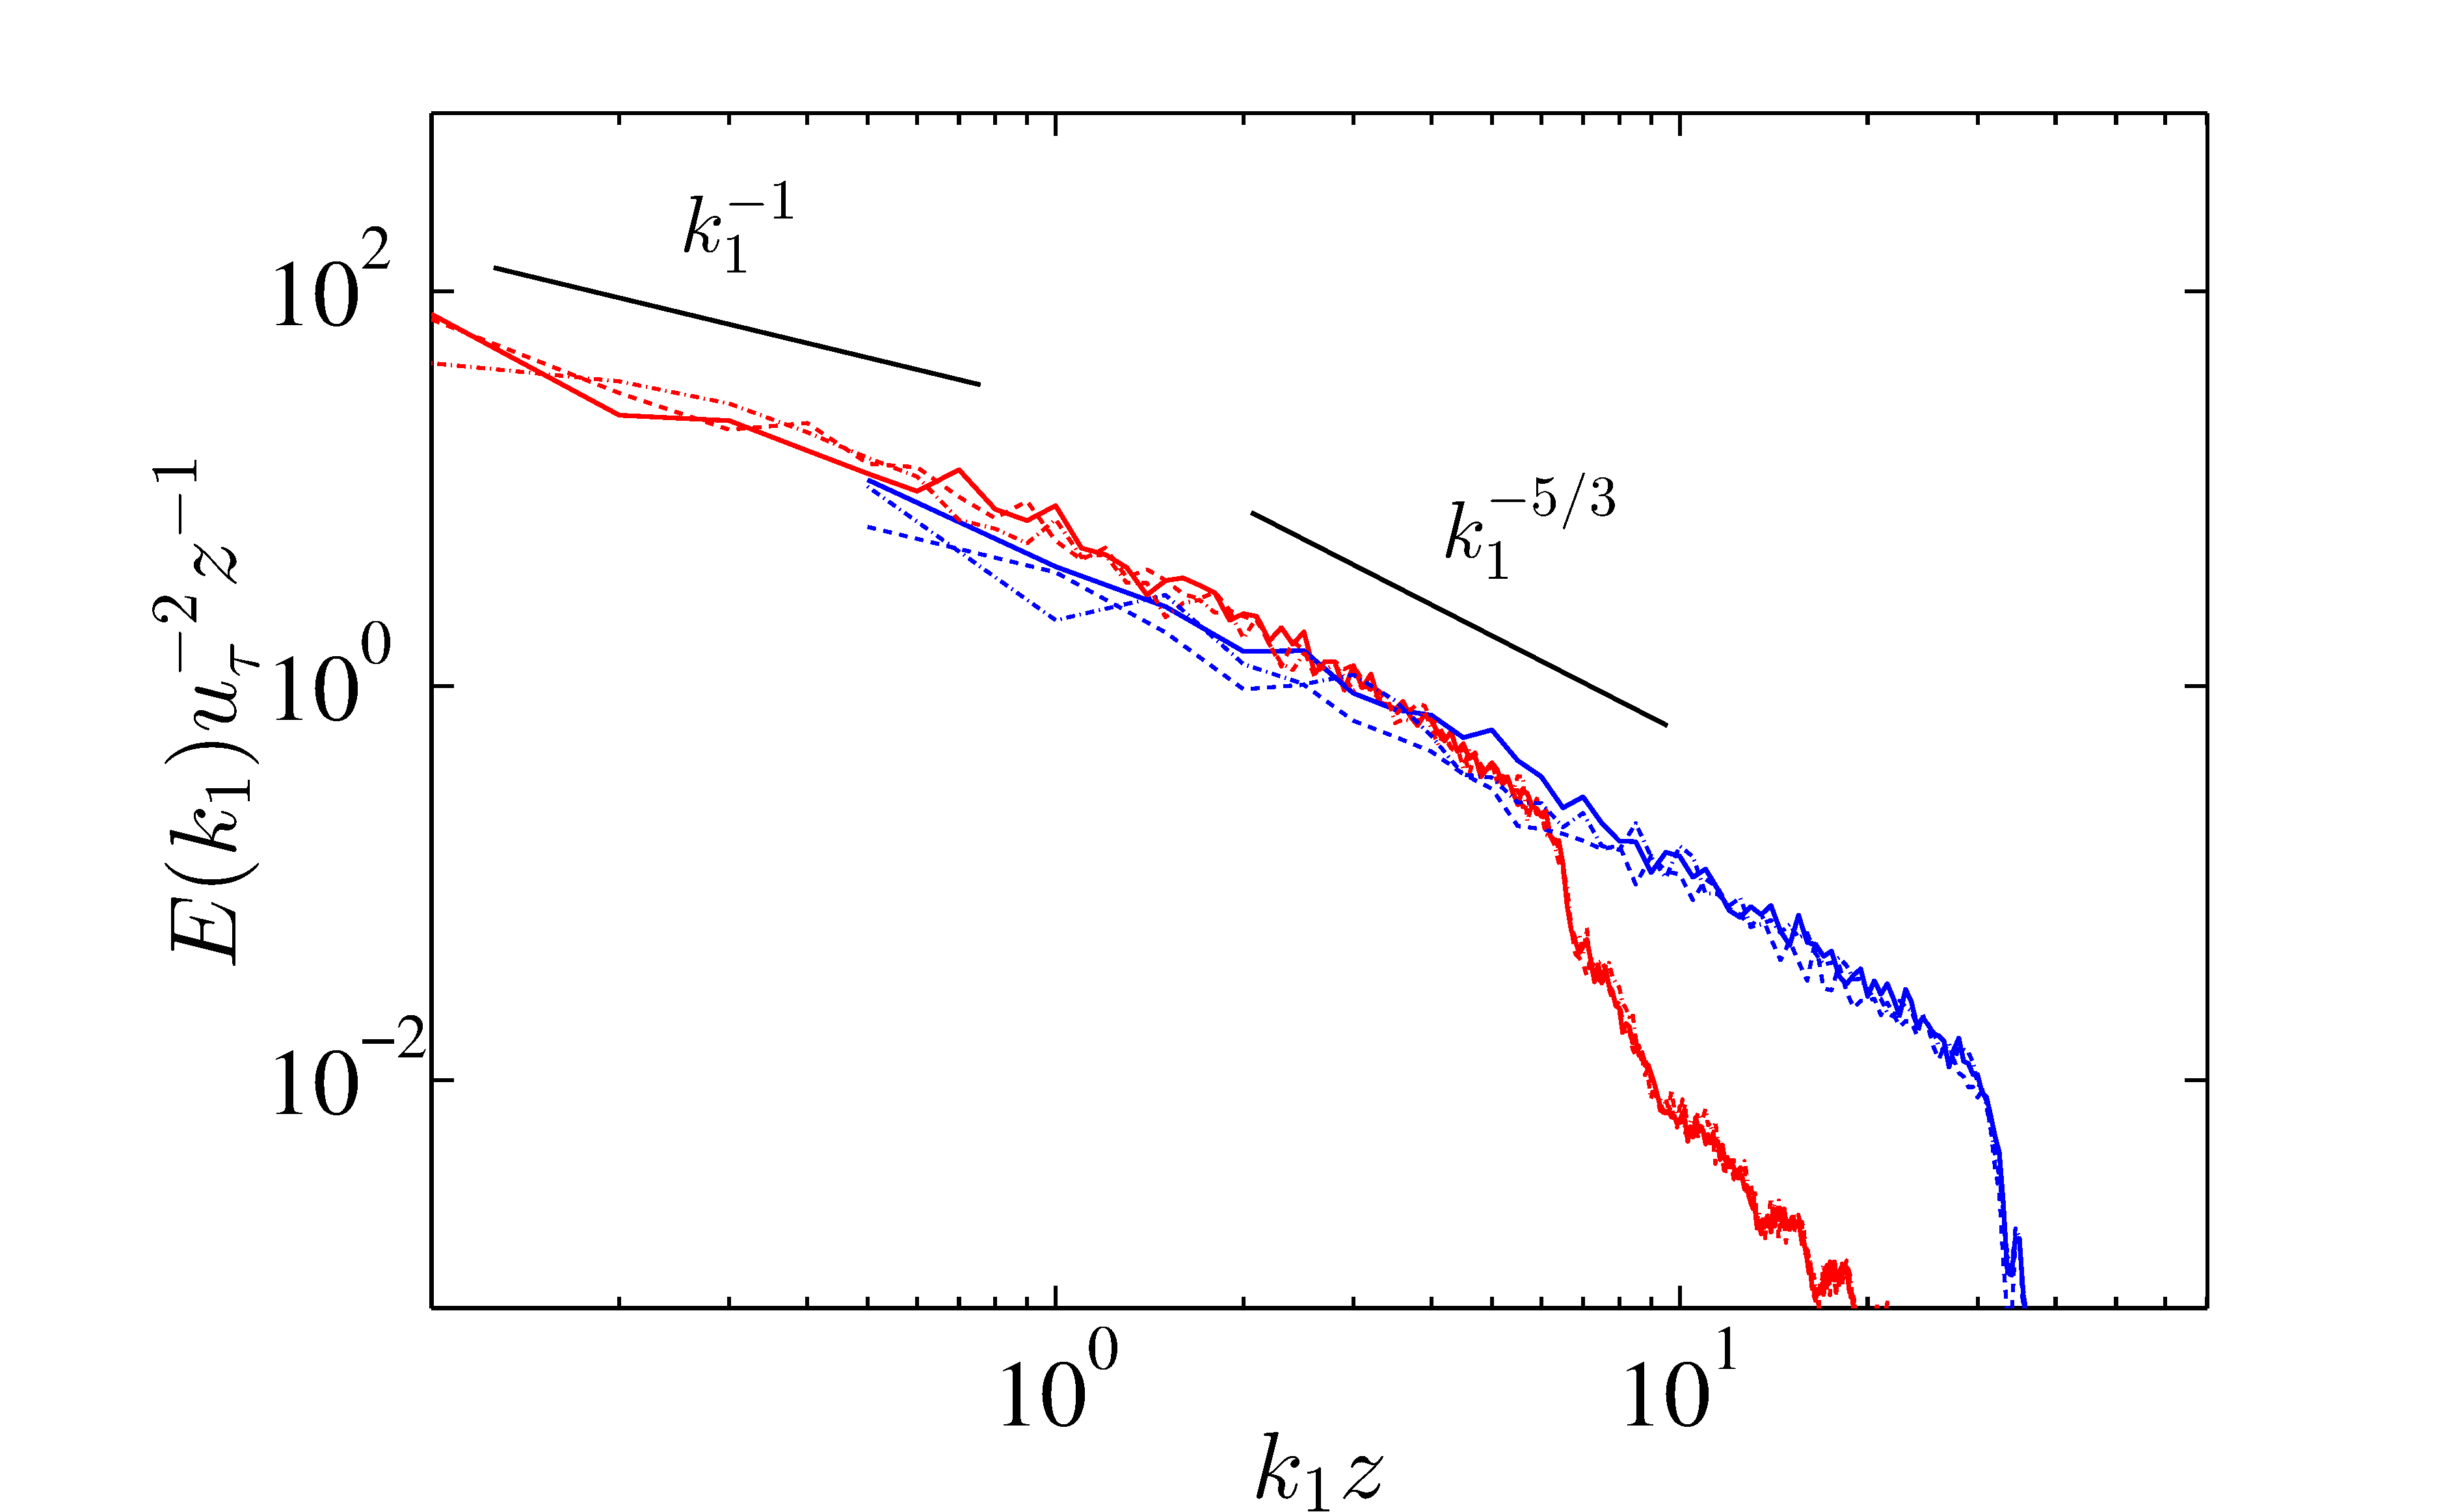
\includegraphics[width=\linewidth]{Figure/energy2.pdf}
                \caption{}
                \label{fig:eng4}
        \end{subfigure}
        \centering
            \begin{subfigure}[b]{0.42\textwidth}
                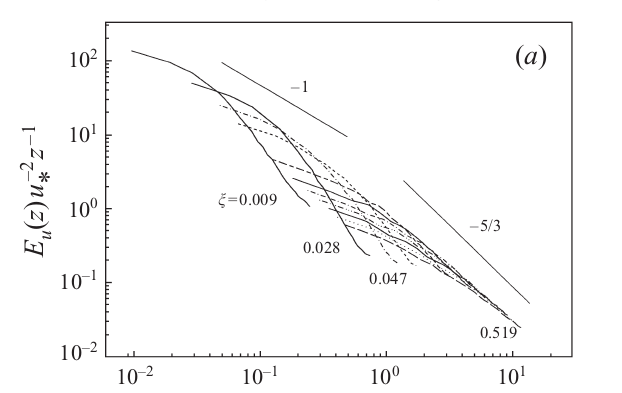
\includegraphics[width=\linewidth]{Figure/porte.png}
                 \caption{}
                 \label{fig:eng_port}
         \end{subfigure}
        \caption{Streamwise energy spectrum of mean velocity in ABL simulations at $Re = 10^{10}$ using mid-point interpolation. (a) $k_{c}=1$ (b) $k_{c}=2$ (c) $k_{c}=4$, for current simulation (SEM) using standard Smagorinsky ($C_s = 0.15, n = 2$) black $-$, $\ z/H = 0.08$; black $--+$, $\ z/H = 0.16$; black $--$,$\ z/H = 0.25$; black $-.$, $\ z/H = 0.41$; black $- \star$, $\ z/H = 0.58$; gray-black $-\circ$, $\ z/H = 0.75$; red-black $-\Box$, $\ z/H = 0.91$; (d) Streamwise energy spectrum of standard Smagorinsky ($C_s = 0.10, n = 2$), Port$\acute{e}$-Agel et al.~\cite{porte1fun}}\label{fig:energy}
\end{figure}

\ack The authors T. Chatterjee and Yulia Peet would like to acknowledge the support of NSF-CBET 13358568 grant for the present work.



\begin{appendices}
  \renewcommand\thetable{\thesection\arabic{table}}
  \renewcommand\thefigure{\thesection\arabic{figure}}
  \numberwithin{equation}{subsection}
  \section{}
  \subsection{Lagrange Interpolants}
  Roots of Lagrange Legendre polynomial for the velocity interpolants
\begin{equation}
(1-\xi^{2})L'_{N}(\xi_j) = 0, \ \ \ \forall \xi_j \in [-1,1]. \label{GLL}
\end{equation}
 Equation~(\ref{GLL}) is solved using Newton-Raphson technique with initial condition of $\xi_j = \cos(j\pi/N), \ \ j = 0,\ldots, N,$ for obtaining a fast convergence. $L'_{N}$ is the first derivative of $N^{th}$ order Legendre polynomial and all the roots lie between $\pm 1$ with a clustering near -1 and 1. These nodes are commonly referred to as Gauss-Lobatto-Legendre (GLL) quadrature points, with the quadrature weights
 
 \begin{equation}
 \rho_j = \frac{2}{N(N+1)}\frac{1}{[L_N(\xi_j)]^2}, \ \ \ \ 0 \le j\le N, \ \ \ \forall \xi_j\in [-1,1]. \label{weights}
 \end{equation}
 The quadrature weights in Equation~(\ref{weights}) are computed as a function of $N^{th}$ order Legendre polynomials at GLL quadrature points. The discrete inner product in 3D thus reduces to
\begin{equation}
(f,g)_{N} = \sum_{i,j,k=0}^{N}\rho_{ijk}f_{ijk}g_{ijk}.\label{galerkin3}
\end{equation}
Here $(f_{ijk},g_{ijk})$ are defined on 3D GLL quadrature nodes on a reference cube and quadrature weights are $\rho_{ijk} = \rho_{i}\rho_{j}\rho_{k}$.
Along the same lines we can define the qudrature points of pressure interpolants as the roots of Legendre polynomial, referred to as Gauss-Legendre (GL) quadrature points.
\begin{equation}
L_{N-1}(\zeta_j) = 0, \ \ \ \forall \zeta_j \in [-1, 1], \ \ 1\le j\le N-1 \label{GL}
\end{equation}
where the roots $\zeta$ are solved using Newton-Raphson method. Consequently, the quadrature weights of GL nodes are given as 
\begin{equation}
\rho^{p}_j = \frac{2}{(1 - \zeta_j^{2})[L'_{N-1}(\zeta_j)]^{2}} \ \ \ \ 1 \le j\le N-1, \ \ \ \forall \zeta_j\in [-1,1]
\end{equation}
with the discrete 3D inner products for $(f,g)_{N,GL}$ being similar to Equation(~\ref{galerkin3}), but with summation from $1$ to $N-1$ using weights $\rho^{p}_{ijk} = \rho^{p}_{i}\rho^{p}_{j}\rho^{p}_{k}$.
\begin{figure}
\centering
        \begin{subfigure}[b]{0.65\textwidth}
                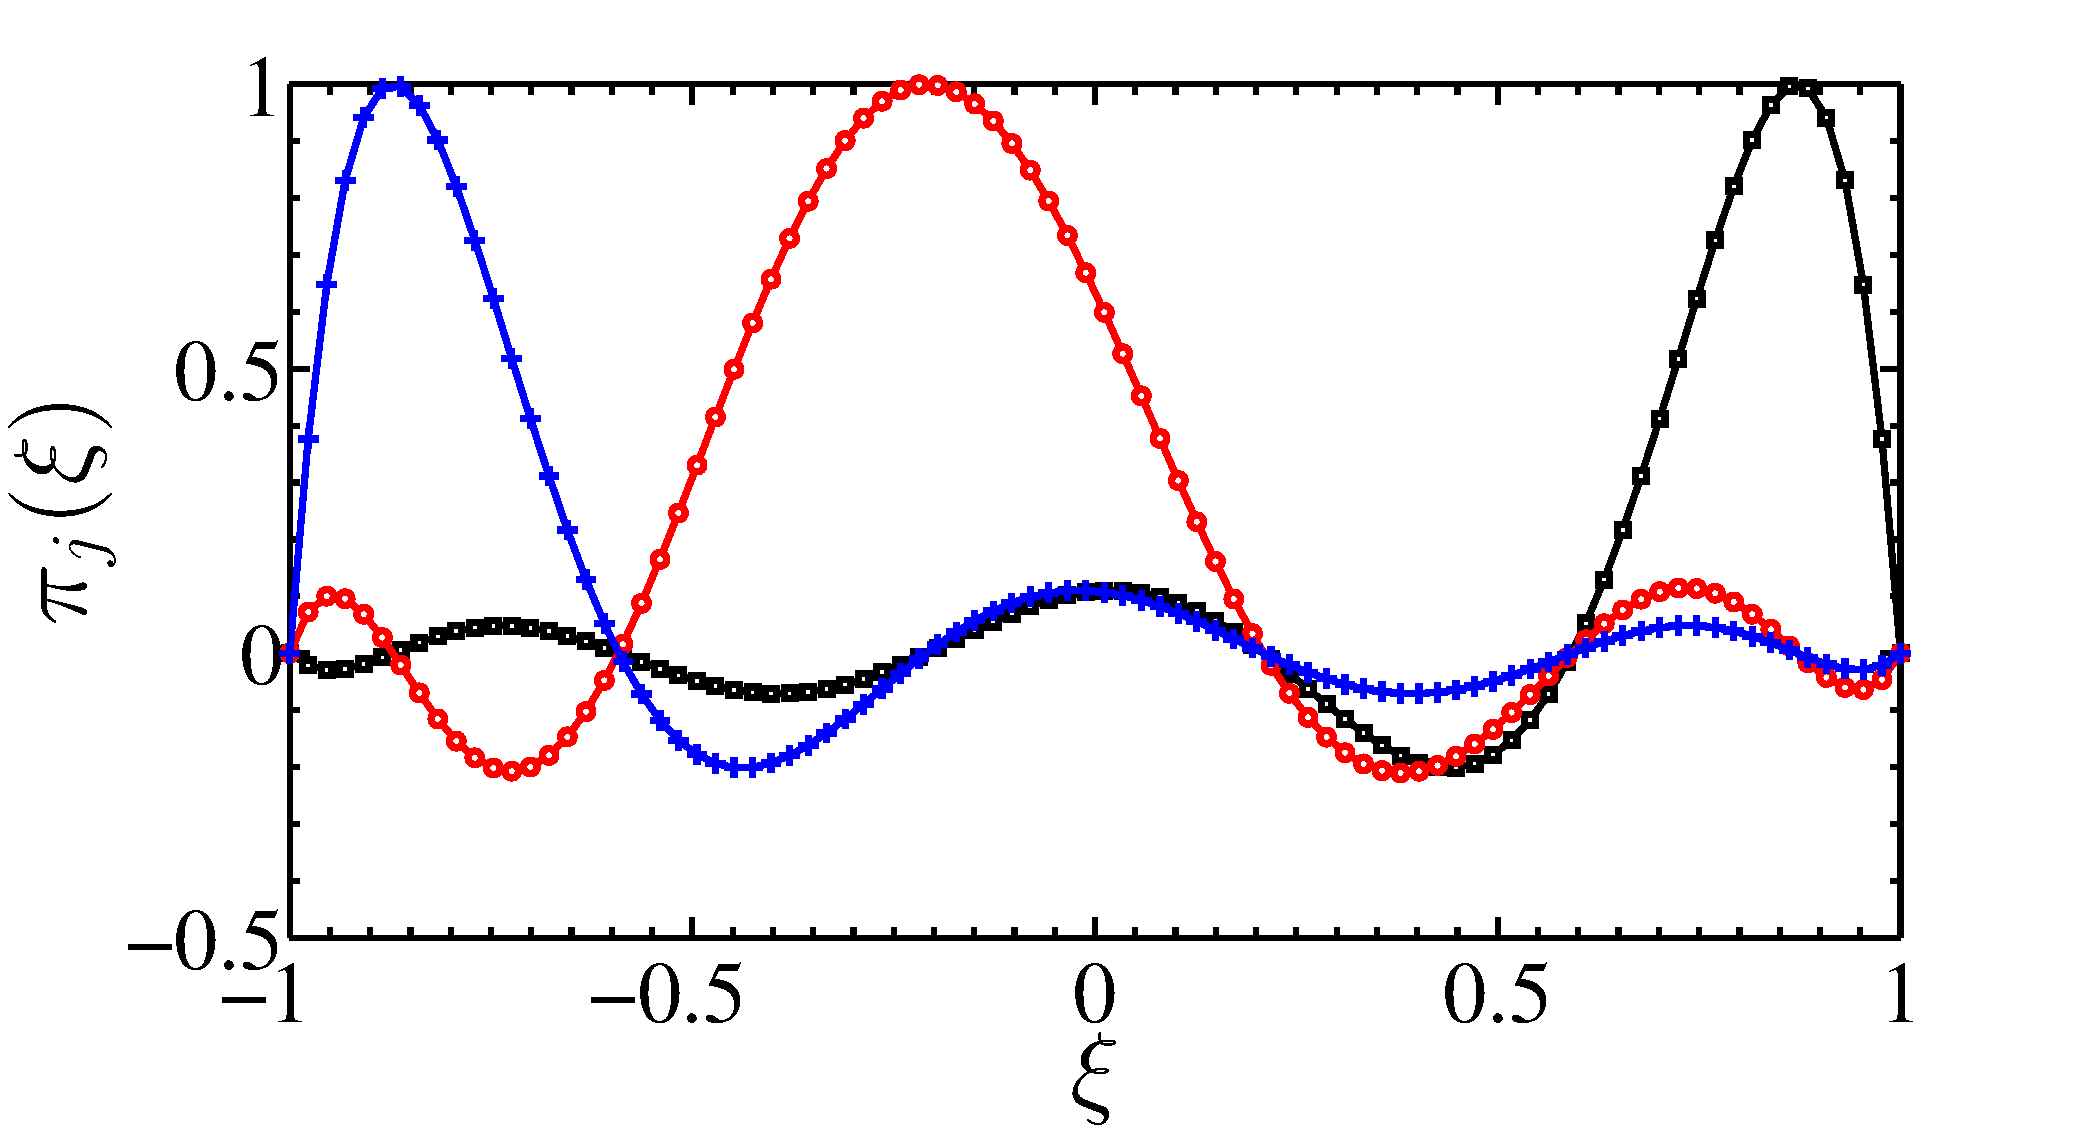
\includegraphics[width=\linewidth]{Figure/legpoly2.pdf}
                \caption{}
                \label{fig:poly1}
        \end{subfigure}
          \begin{subfigure}[b]{0.45\textwidth}
         \centering
                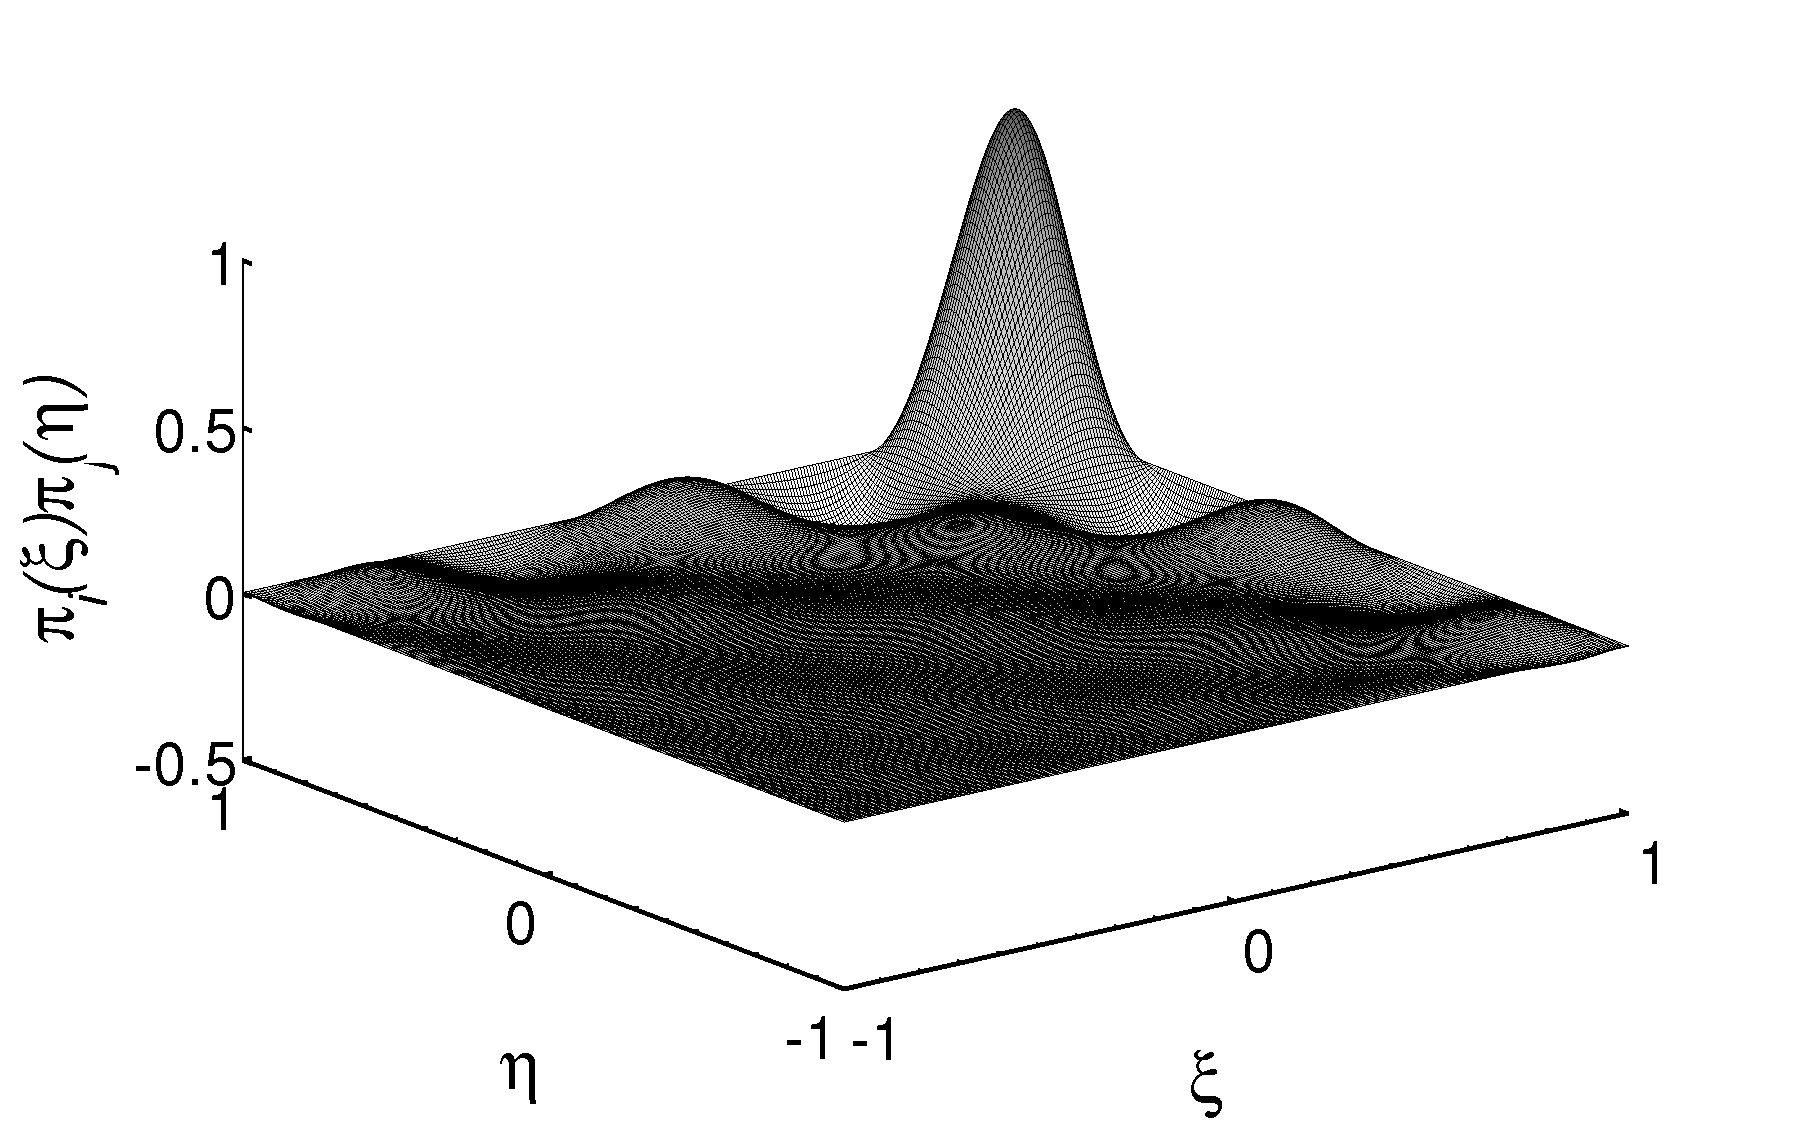
\includegraphics[width=\linewidth]{Figure/legpoly_2D1.pdf}
                 \caption{}
                 \label{fig:poly2}
         \end{subfigure}%
         \begin{subfigure}[b]{0.45\textwidth}
         \centering
                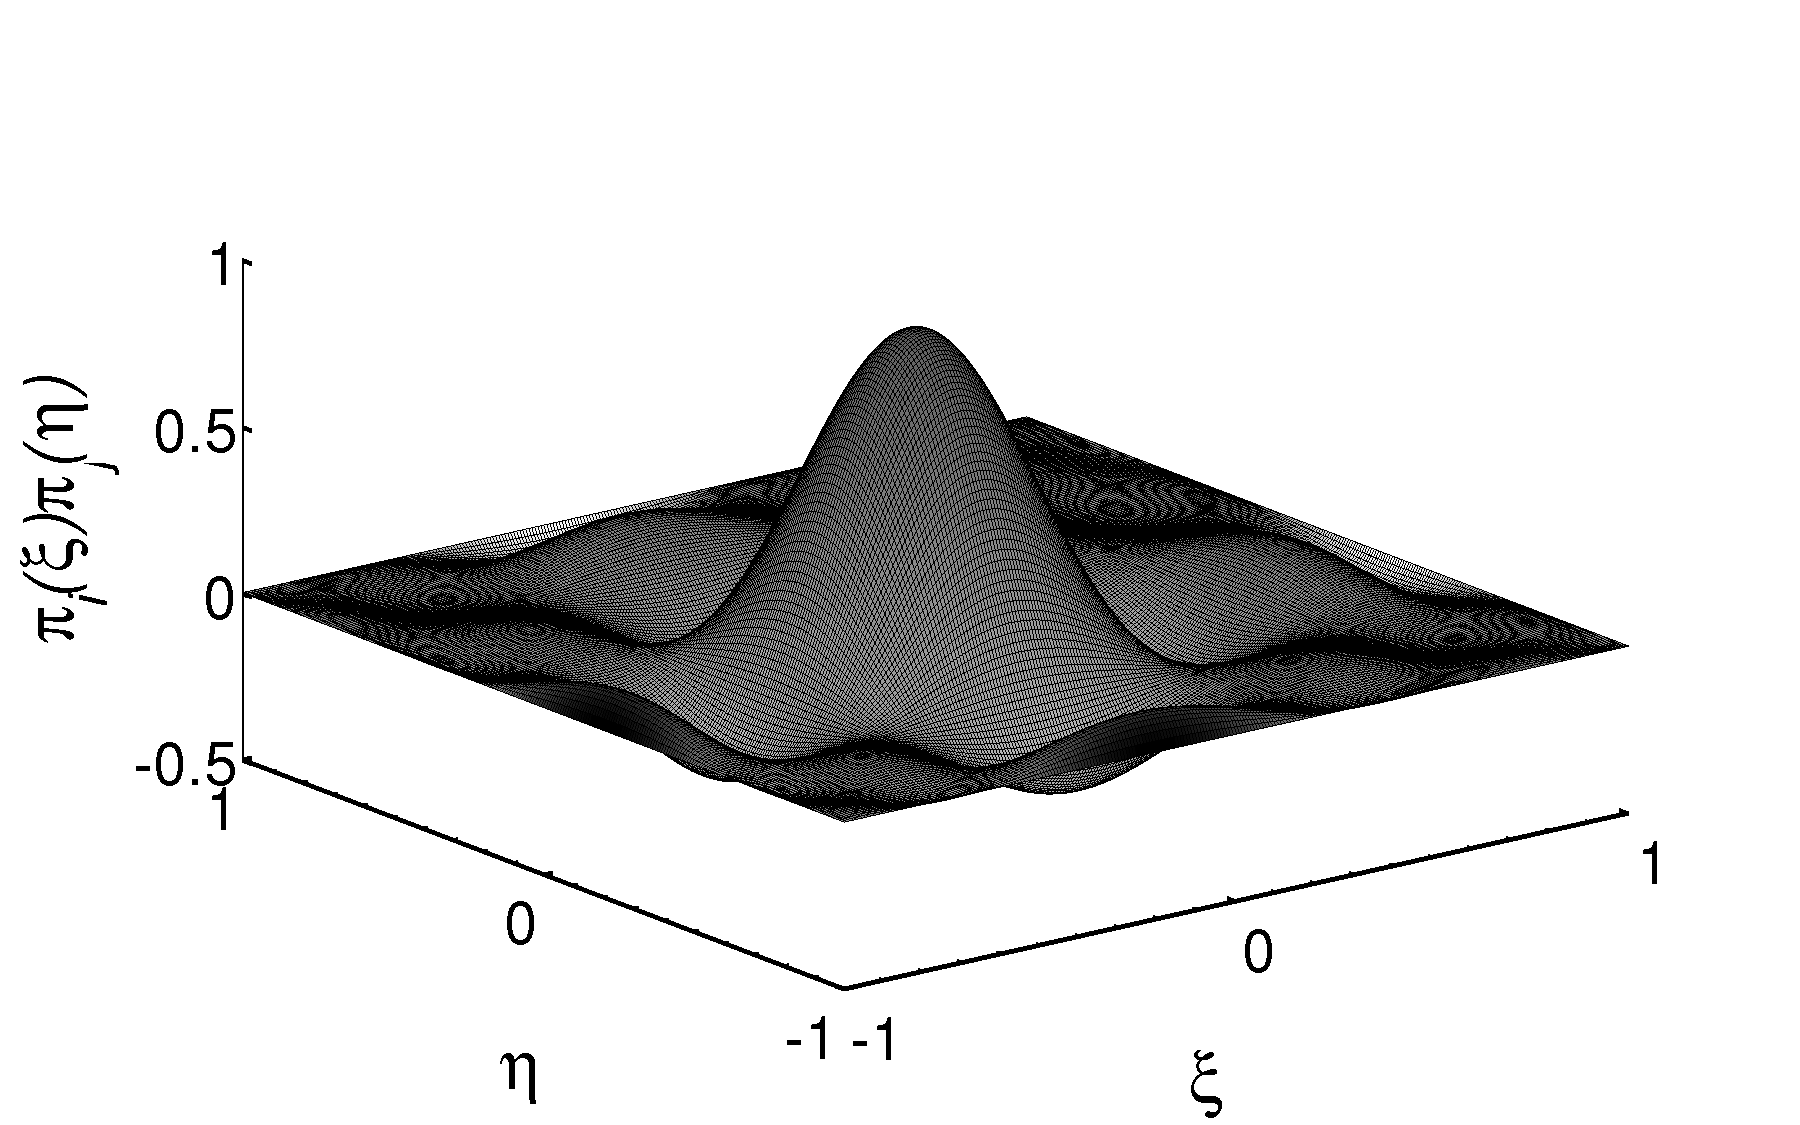
\includegraphics[width=\linewidth]{Figure/legpoly_2D2.pdf}
                 \caption{}
                 \label{fig:poly3}
         \end{subfigure}
        \caption{(a) Lagrange-Legendre polynomial interpolant ${\pi_j}_{j=0}^{N}$ with $N = 7\,(\mbox{polynomial degree})$ in current SEM formulation. Black-gray $--\ocircle$,   $\pi_0(\xi)$;  black $-\Box$,  $\pi_1(\xi)$;  black $--\Diamond$,  $\pi_2(\xi)$;  black $-.*$,  $\pi_3(\xi)$;  black-gray $--\davidsstar$  $\pi_5(\xi)$; gray-black $-$ \ding{72},  $\pi_6(\xi)$; black $+$, $\pi_7(\xi)$; $\pi_j(\xi_i) = \delta_{ij}$. (b)$\  \pi_{1,1}(\xi,\eta) \ \ $ (c) $\  \pi_{4,4}(\xi,\eta) \ $. Figures (b), (c) obtained as Kronecker products of $\pi_{i}(\xi)\otimes \pi_{j}(\eta)$ for 2D case.}\label{fig:figure_legpoly1}
\end{figure}
The basis functions for expansion of the velocity variables correspond to Lagrange-Legendre interpolating polynomials,
\begin{equation}
\pi_{N,j}(\xi) = \prod_{i\neq j}\frac{\xi - \xi_j}{\xi_i - \xi_j} =  \frac{-1}{N(N+1)}\frac{(1-\xi^{2})L'_{N}(\xi)}{(\xi - \xi_j)L_N(\xi_j)}, \ \  \  \   0 \leq j \leq N, \  \  \ \  \xi \in [-1,1],  \label{legendre1}
\end{equation}
where $\xi_j$ are GLL quadrature nodes. Figure~\ref{fig:figure_legpoly1} shows the Lagrange-Legendre basis functions (Equation~(\ref{legendre1})) displaying the cardinality property, and they all have the common intersection point at the GLL quadrature nodes (roots of numerator of basis functions in Equation~(\ref{legendre1}) ) while $\pi_{j}(\xi) \ \mbox{and} \ \pi_{N-j}(\xi)$ basis functions have reflective symmetry about $\xi = 0$.

Likewise, it is legitimate to define the Lagrange interpolant basis functions for the pressure interpolants of degree $N-2$
\begin{equation}
\pi^{p}_{N,j}(\zeta) = \prod_{i\neq j}\frac{\zeta - \zeta_j}{\zeta_i - \zeta_j} = \frac{L_{N-1}(\zeta)}{(\zeta - \zeta_j)L'_{N-1}(\zeta_j)} , \ \  \  \   1 \leq j \leq N-1, \  \  \ \  \zeta \in [-1,1],  \label{legendre1}
\end{equation} 
\par

In 3D, velocity function in the spectral element method in the local element
\begin{equation}
u(r_1,r_2,r_3)|_{\hat{\Omega}} = \displaystyle\sum_{i=0}^{N_x}\sum_{j=0}^{N_y}\sum_{k=0}^{N_z}u_{ijk}^{e}\pi_{N_x,i}({r_1})\pi_{N_y,j}({r_2})\pi_{N_z,k}({r_3}),  \ \ \ {r_1},{r_2},{r_3}\in [-1,1]^3,
\end{equation}
where, $\pi_{N_x,i}(r_1),\hspace{0.5em} \pi_{N_y,j}(r_2), \hspace{0.5em}\pi_{N_z,k}(r_3)$ are the Lagrange polynomial based interpolant of degree $N_x$, $N_y$ and $N_z$ as in Equation(~\ref{legendre1}) satisfying the cardinality property $\pi_{N,i}(\xi_{j}) = \delta_{ij}$ where $\delta_{ij}$ is the Kronecker delta function.
 
Identically the pressure function in SEM in the local element, with $\pi^{p}_{N,j}({\zeta_i}) = \delta_{ij} (\in \mathbb{P}_{N-2})$
\begin{equation}
p(r_1,r_2,r_3)|_{\hat{\Omega}} = \displaystyle\sum_{i=1}^{N_x-1}\sum_{j=1}^{N_y-1}\sum_{k=1}^{N_z-1}p_{ijk}^{e}\pi^{p}_{N_x,i}({r_1})\pi^{p}_{N_y,j}({r_2})\pi^{p}_{N_z,k}({r_3}),  \ \ \ {r_1},{r_2},{r_3}\in [-1,1]^3
\end{equation}

\end{appendices} 
 
 
 
\bibliography{flddoc}
\bibliographystyle{wileyj}


%\begin{thebibliography}{9}

%\bibitem{R1} Kopka~H, Daly~PW. 2003. \emph{A Guide to \LaTeX} (4th~edn).
%Addison-Wesley.

%\bibitem{R2} Lamport~L. 1994. \emph{\LaTeX: a Document Preparation System} (2nd~edn).
%Addison-Wesley.

%\bibitem{R3} Mittelbach~F, Goossens~M. 2004. \emph{The \LaTeX\ Companion}
%(2nd~edn). Addison-Wesley.
%\end{thebibliography}
\end{document}
